
\chapter[ಭಾಗ -  1]{}\label{chap1}

\begin{center}
\rule{5cm}{1pt}\\[5pt]
{\Large\bfseries ಓರಿಗಾಮಿ - ಪ್ರಸ್ತಾವನೆ ಮತ್ತು ಇತಿಹಾಸ }\\[3pt]
\rule{5cm}{1pt}
\end{center}
 
 ಮಾನವನ ನಿತ್ಯ ಜೀವನದಲ್ಲಿ ಗಣಿತವು ಹಾಸುಹೊಕ್ಕಾಗಿದೆ. ಅಲ್ಲದೇ ``ಗಣಿತದಿಂದ ಪ್ರಾರಂಭವಾಗದ ಯಾವದೇ ವಿಷಯವು ನ್ಯೂನತೆಯಿಂದ ಕೂಡಿರುತ್ತದೆ." ಎಂಬ ತಜ್ಞರ ಮಾತಿನಿಂದ ಗಣಿತದ. ಮಹತ್ವ ನಮಗೆ ತಿಳಿದು ಬರುತ್ತದೆ. ಗಣಿತ ಶಾಸ್ತ್ರಕ್ಕೆ  ಚಾಲನೆ ನೀಡಿದ ಸೊನ್ನೆ [0]ಯನ್ನು ಕಂಡುಹಿಡಿದವರು ಭಾರತೀಯರು. ಅಂದೇ ವಿಜ್ಞಾನದ ಪ್ರಾರಂಭಿತ ಖಗೋಳಶಾಸ್ತ್ರವು ಸಂಪೂರ್ಣವಾಗಿ ಗಣಿತವನ್ನೂ ಅವಲಂಬಿಸಿದೆ. ಇಂತಹ ಗಣಿತವನ್ನು ಎಲ್ಲರೂ ತಿಳಿದುಕೊಳ್ಳುವದು ಅವಶ್ಯ. ಇಂದಿನ ಮಕ್ಕಳಿಗೆ ಗಣಿತವು ಕಬ್ಬಿಣದ ಕಡಲೆಯಾಗಿದೆ. ಇದಕ್ಕೆ ಅನೇಕ ಕಾರಣಗಳು ಇವೇ. 
 \begin{itemize} 
 \itemsep=2pt
 \item ಗಣಿತವನ್ನು ಅಮೂರ್ತವಾಗಿ ಬೋಧಿಸುವುದು. 
 
 \item ಗಣಿತ ಕಲಿತೆಗೆ ದಿನ ನಿತ್ಯದ ವ್ಯವಹಾರದ ಉದಾಹರಣೆಗಳನ್ನು ಉಪಯೋಗಿಸದೇ ಇರುವುದು.
 
 \item ವರ್ಗಕೊಣೆಯಲ್ಲಿ ಗಣಿತವನ್ನೂ ಬೋಧಿಸುವಾಗ ಪಾಠೋಪಕರಣಗಳನ್ನು ಉಪಯೋಗಿಸದೇ ಇರುವುದು
 
 \item ಗಣಿತ ಕಲಿಕೆಗೆ ಕಂಠವಾದ ಅಗತ್ಯ ಎನ್ನುವ ಮನೋಭಾವ.

\item ನಿರಂತರ ಅಭ್ಯಾಸದ ಕೊರತೆ.
 
 \item  ಸೇತು ಬಂಧಕ್ಕೆ ಆಧ್ಯತೆ ನೀಡದಿರುವದು.
 
 \item ಗಣಿತದ ಮುಖ್ಯವಾದ ಪರಿಕಲ್ಪನೆಗಳನ್ನು ತಿಳಿದುಕೊಳ್ಳುವದು ಕಠಿಣ.
 
 \item ಗಣಿತದ ತಳಹದಿಯ ಬಗ್ಗೆ ಜ್ಞಾನದ ಕೊರತೆ. 
 
 \item ಗಣಿತದ ಬಗ್ಗೆ ಶಿಕ್ಷಕರೇ ಪೂರ್ವಗ್ರಹ ಪೀಡಿತರಾಗಿರುವದು.
 
 \item ಗಣಿತ ವಿಷಯವು ಉಳಿದ ವಿಷಯಗಳಿಗಿಂತ ಭಿನ್ನ ಸ್ವರೂಪವನ್ನು ಹೊಂದಿದೆ. ಇಲ್ಲಿ ಮೂಲ ತತ್ವಗಳೇ ಸರಿಯಾಗಿ ತಿಳಿಯದಿದ್ದಲ್ಲಿ ವಿದ್ಯಾರ್ಥಿ ಹಿಂದೆ ಉಳಿಯುತ್ತಾನೆ. ಈ ಹಿಂದೆ ಉಳಿಯುವಿಕೆ ಮುಂದಿನ ವರ್ಗಗಳಲ್ಲಿ ಹೆಚ್ಚಾಗುತ್ತಾನೆ ಹೋಗುತ್ತದೆ. 
  
 \item ಗಣಿತದ ಪ್ರಾರಂಭಿಕ ಹಂತದಲ್ಲಿ ಮುಖ್ಯ ಪರಿಕಲ್ಪನೆಗಳ ಬೋಧನೆಯಲ್ಲಿ ಲೋಪವಿದೆ ಎಂದು ``ವಿಶ್ವವಿದ್ಯಾಲಯ ಧನಸಹಾಯ ಆಯೋಗ" [UGC] ದಂತಹ ಸಂಸ್ಥೆಗಳು ತಮ್ಮ ಅಧ್ಯಯನದಲ್ಲಿ ಕಂಡುಕೊಂಡಿವೆ. 
 \end{itemize}
 
 ಮೇಲಿನ ಎಲ್ಲಾ ಕಾರಣಗಳಿಂದ ಮಕ್ಕಳಲ್ಲಿ ಗಣಿತ ಕಲಿಕೆ ಮಟ್ಟವು ಕೆಳಮಟ್ಟಕ್ಕೆ  ಇಳಿದಿದೆ. ಇದನ್ನು ಬಿನ್ನತ ಮಟ್ಟಕ್ಕೆ ಹೆಚ್ಚಿಸಬೇಕೆಂದರೆ ಗಣಿತ ಬೋಧನೆಯ ವಿಧಾನವು ಬದಲಾವಣೆಯಾಗಬೇಕು. ಬದಲಾವಣೆಯ ಮೊದಲ ಹಂತವೇ ಶಾಲೆ ಕಾಲೇಜುಗಳಲ್ಲಿ ``ಗಣಿತ ಪ್ರಯೋಗಾಲಯ" [Maths lab] ಸ್ಥಾಪಿಸುವುದಾಗಿದೆ.
  
 \section*{ಗಣಿತ ಪ್ರಯೋಗಾಲಯ : [Maths Lab]:} ಭೌದ್ಧಿಕ ಮತ್ತು ಮಾನಸಿಕ ನಡುವಳಿಕೆಗಳು ಮತ್ತು ಮಕ್ಕಳಲ್ಲಿ ಕೌಶಲ್ಯಗಳು ಬೆಳೆಯಲು ಸಹಕಾರಿಯಾಗುವ ಚಟುವಟಿಕೆ ಆಧಾರಿತ ಕಲಿಕೆಗೆ ಪ್ರೋತ್ಸಾಹ ತೊಡುವ ವ್ಯವಸ್ಥೆಗೆ ``ಗಣಿತ ಪ್ರಯೋಗಾಲಯ [Maths Lab] ಎಂದು ಕರೆಯುತ್ತಾರೆ. 
 
 ಗಣಿತ ಪ್ರಯೋಗಾಲಯದಿಂದ ನಾವು ಕೆಳಗಿನ ಅನುಕೂಲತೆಗಳನ್ನು ಪಡೆಯುತ್ತೇವೆ.
 \begin{itemize}
 \item ಇದು ಗಣಿತ ಕಲಿಕೆಗೆ ಹಾಗೂ ಬೋಧನೆಗೆ ಪೂರಕ ಸಂದರ್ಭಗಳನ್ನು ಒದಗಿಸುತ್ತದೆ.
 \item ಇದು ಮಗು ಕೇಂದ್ರಿತ [Child centred Education] ಪದ್ಧತಿಯಲ್ಲಿ ಕಲಿಯಲು ಹಾಗೂ ಗುರುಗಳ ಮಾರ್ಗದರ್ಶನದಲ್ಲಿ ಸಮಸ್ಯೆಗಳನ್ನು ತನ್ನಿಂದ ತಾನೆ ಪರಿಹಾರ ಕಂಡುಕೊಳ್ಳಲು ಪ್ರೋತ್ಸಾಹ ಕೊಡುವುದು. 
 \item ಗಣಿತ ಬೋಧನೆಯಲ್ಲಿ ಅಥವಾ ಕಲಿಕೆಯಲ್ಲಿ ಪ್ರಯೋಗ ಅಥವಾ ಚಟುವಟಿಕೆಗಳ ಕೊರೆತಗಳನ್ನು ನೀಗಿಸುತ್ತದೆ. 
 \item ಮುಖ್ಯವಾಗಿ ಇದು ``ಓರಿಗಾಮಿ ವಿಧಾನ"ಕ್ಕೆ ಅವಕಾಶ ಕಲ್ಪಿಸುತ್ತದೆ. ಹೀಗೆ ಗಣಿತ ಪ್ರಯೋಗಾಲಯವನ್ನು ಉಪಯೋಗಿಸಿ ಗಣಿತವು ಕಬ್ಬಿಣ ಕಡೆಲೆಯಲ್ಲ ಇದೊಂದು ಕಬ್ಬಿನ ಸಿಹಿ ಎಂಬುದನ್ನು ತಿಳಿಸು ಕೊಳ್ಳಬೇಕಾಗಿದೆ. 
 \end{itemize}


\section*{``ಓರಿಗಾಮಿ"ಯ ಇತಿಹಾಸ [History of Origami]}
``ಓರಿಗಾಮಿ" [Origami] ಎಂಬ ಶಲ್ಧವು ಇಂದು ಎಲ್ಲರೂ ಚರ್ಚಿಸುವ ವಿಷಯವಾಗಿದೆ. ಇತರ ಕಲೆಗಳಂತೆ ಕಾಗದ ಮಡಚುವ ಕಲೆಯು ಮಾನವ ತೃತಿಯಂತೆ ಎಲ್ಲಿಯೂ ಸಂಗ್ರಹವಾಗಿಲ್ಲ. ಓರಿಗಾಮಿ ಕಲೆ ಎಲ್ಲಿ ಪ್ರಾರಂಭವಾಯಿತು ಮತ್ತು ಯಾರು ಯಾವಾಗ ಕಂಡುಹಿಡಿದರು ಎಂಬ ಸಂಗತಿಗಳು ನಮಗೆ. ಇಲ್ಲಿಯವರಗೂ ತಿಳಿದುಬಂದಿಲ್ಲ. ಇಲ್ಲಿ ನಾವು ಹೇಳಲು ಹೊರಟಿಸುವ ಸಂಗತಿಗಳು ಓರಿಗಾಮಿಯ ಪೂರ್ಣವಿವರಗಳನ್ನು ಕೊಡುತ್ತವೆ ಎಂದು ನಾನು ನಂಬಲ್ಲ. ಆದರೆ ಜಾನ್ ಸ್ಮಿತ್ [John Smith], ಡೇವಿಡ್ ಲಿಸ್ಟರ [Devid Lister] ಮತ್ತು ಕೋಶಿರೋ ಹಟೇರಿ [Koshiro Hatori] ಇವರು ಓರಿಗಾಮಿಯ ಬಗ್ಗೆ ಪೂರ್ಣ ಪ್ರಮಾಣದಲ್ಲಿ ಮಾಹಿತಿಕೊಡಲು ಪ್ರಯತ್ನಿಸಿದ್ದಾರೆ. 

ಒಂದು ಸಂಗತಿಯನ್ನು ನೆನಪು ಮಾಡಿಕೊಳ್ಳಲೇ ಬೇಕು ಏನೆಂದರೆ ಕಾಗದದ ಸಂಶೋಧನೆ ಆದ ನಂತರ ಓರಿಗಾಮಿ ಕಲೆ ಪ್ರಾರಂಭವಾಗಿರಬೇಕು. ಕಿೃ.ಶ. 105 ರಲ್ಲಿ ಚೀನಾದಲ್ಲಿ ಪ್ರಥಮವಾಗಿ ಕಾಗದವನ್ನು ಕಂಡುಹಿಡಿದು ಉಪಯೋಗಿಸಲಾಯಿತು. ಆದರೆ ಪ್ರಾಚೀನ ವಸ್ತು ಶಾಸ್ತ್ರದ ಪುರಾವೇಗಳಿಂದ ಕಾಗದವನ್ನು ಇದಕ್ಕೂ ಮೊದಲೇ ಕಂಡುಕೊಳ್ಳಲಾಗಿದೆ. ಎಂಬ ಸಂಗತಿಯು ತಿಳಿದು. ಬರುತ್ತದೆ. ಓರಿಗಾಮಿ ಕಲೆಯು ಜಪಾನಿನ ಕಲೆ ಎಂದು ನಾವು ತಿಳಿದು ಕೊಂಡಿದ್ದೇವೆ. ಕಾರಣ ಇದು ಜಪಾನಿನಲ್ಲಿ ಪ್ರಾರಂಭವಾಗಿರ ಬಹುದೆಂದು ನಂಬಿದ್ದೇವೆ. ಆದರೆ ಓರಿಗಾಮಿ ಕಲೆಯು ಚೀನಾದಿಂದ ಜಪಾನಿಗೆ ಬಂದ ಕಲೆಯಾಗಿರುತ್ತದೆ. ಕಿೃ.ಶ. 1100 ನೇ ಮೇ ತಿಂಗಳಲ್ಲಿ ಚೀನಾದಲ್ಲಿ ಪ್ರಾರಂಭವಾಗಿ ಜಗತ್ತಿನ ಎಲ್ಲ ರಾಷ್ಟ್ರಗಳಲ್ಲಿ  ಇಂದಿಗೂ ಓರಿಗಾಮಿ ಕಲೆ ಉಪಯೋಗವಾಗುತ್ತಾ ನಡೆದಿದೆ. 

``ಓರಿಗಾಮಿ"ಯ ಬಗ್ಗೆ ಯಾಗಲಿ, ಕಾಗದ ಮಡಚುವಿಕೆ ಬಗ್ಗೆಯಾಗಲಿ, ಚೀನಾದಲ್ಲಿ ಕಡಿಮೆ ಪುರಾವೆಗಳು ಇವೆ. ಆದರೂ ``ಯುಂಬಾಯೇ" [Yuanbao] ನ ಉದಾಹರಣೆಯು. ಅತೀ ಹಳೆಯ ಸಾಕ್ಷಿಯು ಚೀನಾದಲ್ಲಿ ದೊರೆತಿದೆ. 17 ನೇ ಶತಮಾನದಲ್ಲಿ ಪ್ರಕಟವಾದ ``Kanamodo" ಪುಸ್ತಕವು ಓರಿಗಾಮೀ ಕಲೆಯ ಬಗ್ಗೆ ಕೆಲವು ಮಾರ್ಗದರ್ಶನ ಸೂಚನೆಗಳನ್ನು ಮಾತ್ರ ಹೊಂದಿತ್ತು. ಕಿೃ.ಶ. 1797 ರಲ್ಲಿ ಪ್ರಕಟವಾದ ಪುಸ್ತಕ  "Hiden-Senbazuru Orikata" ಎಂಬುದು ಬಹಳ ಹಳೆಯ ಪುಸ್ತಕವಾಗಿದ್ದು. ಇದು ಜಪಾನಿನಲ್ಲಿ ಒಬ್ಬರ  ಕೈಯಿಂದ ಇನ್ನೊಬ್ಬರ ಕೈಗೆ ವರ್ಗಾವಣಿಗೊಂಡು ಓರಿಗಾಮಿ ಕಲೆ ಹೆಚ್ಚು ಪ್ರಚಾರವಾಗಿದ್ದರಿಂದ ಇದು ಜಪಾನಿನ ಕಲೆಯಂದು ಇಂದಿಗೂ ತಿಳಿದುಕೊಳ್ಳಲಾಗುತ್ತದೆ. 

ಪ್ರಾರಂಭದಲ್ಲಿ ಈ ಕಲೆಯನ್ನು ಮದುವೆ ಹಾಗೂ ಇತರೇ ಸಭೆ ಸಮಾರಂಭಗಳಲ್ಲಿ ಅಲಂಕಾರ ಮಾಡಲು ಬಳಸಲಾಗುತ್ತಿತ್ತು. ಇದು ಯುವಕರಲ್ಲಿ ತಮ್ಮ ಜ್ಞಾನ ಅಥವಾ ಕಲ್ಪನೆ ಇವುಗಳ ಜೊತೆಗೆ ಕೈಬೆರಳುಗಳ ಕೌಶಲ್ಯಗಳನ್ನು ಬೆಳಸಿಕೊಳ್ಳಲು ಸಹಕಾರಿಯಾಯಿತು. ಜಪಾನಿನಲ್ಲಿ ಓರಿಗಾಮಿ ಕಲೆಯನ್ನು ಕಲಿಸಲು ಅಥವಾ ತರಬೇತಿ ಕೊಡಲು ಪ್ರಾಥಮಿಕ ಹಾಗೂ ಪ್ರೌಢ ಶಾಲಾಹಂತಗಳಲ್ಲಿ ಸಂಸ್ಥೆಗಳು ಇವೆ. ಇವುಗಳ ಮೂಲಕ ಮಕ್ಕಳು ತಮ್ಮ ಕೈ ಬೆರಳುಗಳಿಗೆ ತರಬೇತಿ ಕೊಡುವ ವಿಧಾನಕ್ಕೆ ``Five Motor Skill" ಎಂದು ಕರೆಯುತ್ತಾರೆ. ಆದರೆ ಆಗ ಈ ಕಲೆಯನ್ನು ಪಠ್ಯವಸ್ತು ಎಂದು ತಿಳಿದುಕೊಳ್ಳಲಾಗಲಿಲ್ಲ. ಎರಡನೇ ಮಹಾಯುದ್ದಕ್ಕಿಂತ ಮೊದಲು ಓರಿಗಾಮಿ ಕಲೆ ಜಗತ್ತಿನಲ್ಲಿ ಹೆಚ್ಚು ಪ್ರಚಾರವಾಗಲಿಲ್ಲ. ಆದರೆ ಮಹಾಯುದ್ಧದ ನಂತರ ಪ್ರಾಂತೀಯ ತಿರುವು ಉಂಟಾಗಿ ಬೇರೆಬೇರೆ ರಾಷ್ಟ್ರದ ಜನರು ಜಪಾನಿಗೆ ಆಗಮಿಸ ತೊಡಗಿದರು. ಅಲ್ಲದೇ  ಜಪಾನಿನ ಯುವಕರು ಇತರೇ ದೇಶಗಳಿಗೆ ಪ್ರವಾಸವನ್ನು ಕೈಕೊಂಡಿದ್ದರಿಂದ ಈ ಕಲೆ ಎಲ್ಲ ದೇಶಗಳಲ್ಲಿ ಪ್ರಚಾರವಾಗಲು ಸಾಧ್ಯವಾಯಿತು. ಜಪಾನಿನ ಯುವಕರು ರಾಯಭಾರಿಗಳಂತೆ ವರ್ತಿನೆ ತಮ್ಮ ಕೈಬೆರಳುಗಳು ಮಾತನಾಡುವಂತೆ ಮಾಡಿದ್ದರಿಂದ ಈ ಕಲೆ ಹೆಚ್ಚು ರಾಷ್ಟ್ರಗಳಲ್ಲಿ ಪ್ರಚಾರವಾಯಿತು. 

ಕಿೃ.ಶ. 1950 ರಿಂದ 1960 ರ ವರಗೆ ಬಹಳಷ್ಟು ಓರಿಗಾಮಿ ಪುಸ್ತಕಗಳು ಇಂಗ್ಲೀಷದಲ್ಲಿ ದೊರಕ ಹತ್ತಿದವು. ಮುಂದೆ 1970 ರಿಂದ 1980 ರ ವರೆಗೆ ಇನ್ನಷ್ಟು ಪುಸ್ತಕಗಳು ದೊರಕ ಹತ್ತಿದವು. ಈ ಕಾರಣಗಳಿಂದ 21 ನೇ ಶತಮಾನಕ್ಕಿಂತ ಪೂರ್ವದಲ್ಲಿ 100 ಕ್ಕಿಂತ ಹೆಚ್ಚು ಪುಸ್ತಕಗಳು ದೊರಕ ಹತ್ತಿದವು. ಈಗ ಸುಮಾರು 30,000 ಕ್ಕಿಂತ ಹೆಚ್ಚಿನ ಸಂಖ್ಯೆಯ ಓರಿಗಾಮಿ ಕೃತಿಗಳು ನಮಗೆ ದೊರಕುತ್ತವೆ. ಅಲ್ಲದೇ ಪ್ರತಿವರ್ಗ ಹೆಚ್ಚಿನ ಸಂಖ್ಯೆಯ ಓರಿಗಾಮಿ ಕೃತಿಗಳು ಹೊರಬರುತ್ತದೆ. 

\section*{ಜಪಾನಿನಲ್ಲಿ ಕಾಗದ ಮಡಚುವಿಕೆ : [Paper folding in Japan]} 
6 ನೇ ಶತಮಾನದಲ್ಲಿ ಕಾಗದವು ಕೋರಿಯಾ ನಂತರ ಜಪಾನಿನಲ್ಲಿ ``ಭೌಧ್ಯ ಸನ್ಯಾಸಿ"ಗಳಿಂದ ಪರಿಚಯವಾಯಿತು. ಆಗ ಕಾಗದ ಮಡಚುವ ಕಲೆ ``ಓರಿಗಾಮಿ ಒಂದು ಕಲೆಯಾಗಿ ಹೊರ ಹೊಮ್ಮಿತು. ಇನ್ನು ಒಂದು ಮುಖ್ಯವಾದ ಸಂಗತಿ ಏನೆಂದರೆ, ಜಪಾನಿನಲ್ಲಿ ಕಾಗದದ ಬೆಲೆ ಅತಿ ಹೆಚ್ಚಾಗಿದ್ದು ಅದು ಸುಲಭವಾಗಿ ದೊರಕುತ್ತಿರಲಿಲ್ಲ ಆದರೂ ಕಾಗದ ಮಡಚುವ ಕಲೆ ಸಭೆ ಸಮಾರಂಭಗಳಲ್ಲಿ ಹಾಗೂ ಸಾಮಾನ್ಯ ಕಾರ್ಯ ಕ್ರಮಗಳಲ್ಲಿ ರೋಮಾಂಚನ ಉಂಟು ಮಾಡುತ್ತಿತ್ತು. 

ಭೌದ್ಧ ಧರ್ಮದಿಂದ ಹೊರದೂಡಲ್ಪಟ್ಟ ಜಪಾನಿನ ಧರ್ಮದ ಮದುವೆಗಳಲ್ಲಿ ಅಲಂಕಾರಕ್ಕಾಗಿ ಕಾಗದದ ಪತಂಗಗಳನ್ನು ಬಳಸುತ್ತಿದ್ದರು. ಈ ಪತಂಗಗಳಿಗೆ  "Mecho" ಮತ್ತು  "Ocho" ಎಂದು ಕರೆಯುತ್ತಾರೆ. ``Mecho" ಪತಂಗವನ್ನು ವರನಿಗೆ ಮತ್ತು "Ocho" ಪತಂಗವನ್ನು ವಧುವಿಗೆ ಉಡುಗರೆಯಾಗಿ ಕೊಡುತ್ತಿದ್ದರು. ಅಲ್ಲದೇ ತಮ್ಮ ಹಿರಿಯರನ್ನು ಪೂಜಿಸಲು ವಿಧ ವಿಧವಾದ ಪ್ರಾಣಿ-ಪಕ್ಷಿಗಳನ್ನು ಕಾಗದದಲ್ಲಿ ಮಡಚಿ ಅರ್ಪಿಸುವ ರೂಢಿ ಇದೆ. ಹಾಗೂ ಸಾಮಾಜಿಕ ಹಬ್ಬಗಳಲ್ಲಿ ಒಬ್ಬರಿಗೊಬ್ಬರು ಹಾರೈಸುವಾಗ ಓರಿಗಾಮಿಯ ಮಾದರಿಗಳನ್ನು ಉಡುಗರೆಯಾಗಿ ಕೊಡುತ್ತಾರೊ. 

``ಜಪಾನ್ ಪೌಂಡೇಶನ್" ಓರಿಗಾಮಿ ಕಲೆಯನ್ನು ಪ್ರೋತ್ಸಹಕೊಡುವ ಉದ್ದೇಶದಿಂದ ಪ್ರತಿವರ್ಗ ಶ್ರೇಷ್ಠ ಓರಿಗಾಮಿ ಮಾದರಿಗಳ ಸ್ಪರ್ಧೆಯನ್ನು ಏರ್ಪಡಿಸುತ್ತಾರೆ. ಅಲ್ಲದೇ ಪ್ರವಾಸಿಗರನ್ನು ಆಕರ್ಷಿಸಲು ಶಾಶ್ವತವಾದ ಓರಿಗಾಮಿ. ವಸ್ತು ಸಂಗ್ರಾಹಾಲಯವನ್ನು ಏರ್ಪಡಿಸುತ್ತಾರೆ. ಈ ಎಲ್ಲ ಕಾರಣಗಳಿಂದ ಜಪಾನಿನಲ್ಲಿ ಕಾಗದದ ಬೇಡಿಕೆ ಹೆಚ್ಚಾಗಿ ``ಗೃಹ ಉದ್ಧೇಮೆ" [Home Industry] ಯಾಗಿ ಪರಿವರ್ತನ ಗೊಂಡಿದೆ. ಈ ಕಾರಣದಿಂದ ಜಪಾನಿನಲ್ಲಿ ವ್ಯಕ್ತಿಗತವಾಗಿ ಆರ್ಥಿಕ ಸುಧಾರಣೆಯಾಗಿದೆ. ಕಿೃ.ಶ. 1797 ರಲ್ಲಿ ವಿನೋದ ಉಂಟುಮಾಡು ಕಾಗದ ಮಡಚುವಿಕೆಯ 1000 ಉದಾಹರಣೆಗೊಳಗೊಂಡ ಪುಸ್ತಕವು "Folding of 1000 Cranes"  ಪ್ರಥಮವಾಗಿ ಪ್ರಕಟನೆಗೊಂಡಿತು. ಮುಂದೆ ಕಿೃ.ಶ. 1845 ರಲ್ಲಿ "Window on Midwinter" ಎಂಬ ಪುಸ್ತಕಗಳು ಸರಣಿ ರೂಪದಲ್ಲಿ ಪ್ರಕಟನೆಗೊಂಡವು. ಇದಾದ ನಂತರ ``ಓರಿಗಾಮಿ" ಕಲೆ ಸರಿಯಾದ ದಾರಿಯಲ್ಲಿ ಸಾಗಿತು. ಯುರೋಪಿಯನ್ ರು ಸಹ ಕಾಗದ ಮಡಚುವಿಕೆಯ ವಿಚಾರಗಳನ್ನು ಹಾಗೂ ವಿಧಾನಗಳನ್ನೂ ರೂಢಿ ಮಾಡಲು ಪ್ರಾರಂಭಿಸಿದರು. 

\section*{ಯುರೋಪಿನ ಕಾಗದ ಮಡಚುವಿಕೆ [Paper folding in Europe]}
ಜಪಾನಿನಲ್ಲಿ ಯಾವ ಸಮಯದಲ್ಲಿ ಕಾಗದ ಮಡಚುವಿಕೆ ಪ್ರಾರಂಭವಾಗಿದಿಯೋ ಅದೇ ಸಮಯದಲ್ಲಿ ಯುರೋಪದಲ್ಲಿಯಾ ಸಹ ಪ್ರಾರಂಭವಾಗಿದೆ. ಈ ಎರಡು ರಾಷ್ಟ್ರಗಳು ಸ್ವತಂತ್ರವಾಗಿ ಮಡಚುವಿಕೆ ಕಲೆಯನ್ನು ಕರೆಗತ ಮಾಡಿಕೊಂಡು ಪ್ರಚಾರ ಮಾದಿದವು. ಕಿೃ.ಶ. 1490 ರಲ್ಲಿ ಪ್ರಥಮವಾಗಿ ಕಾಗದ ಮಡಚುವಿಕೆ ಕಲೆಯು ಪ್ರಕಟನೆಯಾಗಿತ್ತು. ಅದರ ಕೆಲವು ಮಾದರಿಗಳು ಜಪಾನಿಗಿಂತ ಮೊದಲೇ ಯುರೋಪಿನಲ್ಲಿ ಪ್ರಚಾರವಾಗಿದ್ದವು. ಜರ್ಮನಿ ಹಾಗೂ ಯುರೋಪಿನಲ್ಲಿ ಹಾಗೂ ಇತರ ಭಾಗಗಳಲ್ಲಿ ಮಕ್ಕಳು ತಮ್ಮ ತಮ್ಮ ಪಾಲಕರಿಂದ ``ಜ್ಞಾನ ಸ್ನಾನ" ಅಥವಾ ಕೃಸ್ತಸ್ನಾನ [baptism]  ಎಂದು ಕರೆಯುವ ``patenbriets" ಎಂಬ ಪ್ರಶಸ್ತಿ ಪತ್ರಗಳನ್ನು ಪಡೆಯುವ ಪದ್ಧತಿ ರೂಢಿಯಲ್ಲಿ ಇತ್ತು. ಈ ಪ್ರಶಸ್ತಿ ಪತ್ರಗಳು (3 $\times$ 3) ಅಥವಾ  (4 $\times$ 4)  ರೀತಿಗಳಲ್ಲಿ ಚೌಕಟ್ಟಿನ ಆಕಾರದಲ್ಲಿ ಮಡಿಕೆಯಾಗಿದ್ದವು. ಈ ಪದ್ಧತಿ ಮುಂದೆ 17 ನೇ ಮತ್ತು 18 ನೇ ಶತಮಾನದ ವರಗೆ ಮುಂದುವರಿಯಿತು. 

ಜಪಾನ ಮತ್ತು ಚೀನಾದಲ್ಲಿ ಕಾಣದೇ ಇರುವ ಓರಿಗಾಮಿ ಮಾದರಿಗಳು ಯುರೋಪಿನಲ್ಲಿ ಪ್ರಚಾರದಲ್ಲಿ ಇದ್ದವು. ಕಿೃ.ಶ. 1806 ರಲ್ಲಿ ಚೀನಿಯರು ಬಳಸುತ್ತಿದ್ದ (4 $\times$ 4) ಚೌಕಟ್ಟಿನ ಚಿಕ್ಕದೋಣಿಯು ಸಹ ಯುರೋಪಿಗೆ ಮಾದರಿಯಾಗಿತ್ತು.

ಓರಿಗಾಮಿ ಕಲೆಯು ಯುರೋಪಿನಿಂದ ದಕ್ಷಿಣ ಆಫ್ರಿಕಾ ನಂತರ ದಕ್ಷಿಣ ಅಮೇರಿಕಾ ಹಾಗೂ ಉತ್ತರ ಅಮೇರಿಕಾ ದೇಶಗಳಿಗೆ ಪ್ರಚಾರವಾಯಿತು. ಕಿೃ.ಶ. 1950 ರಲ್ಲಿ  ``Akira Yoshizana" ಮತ್ತು "Sam Randleft"  ಇವರು ಮಡುಚುವಿಕೆಯಿಂದ ಕಾಗದದ ಮಾದರಿಗಳನ್ನು ತಯಾರಿಸಲು ಬೇಕಾಗುವ ವಿಧಾನಗಳ ಬಗ್ಗೆ  [Origami Symbols] ಪುಸ್ತಕ ರೂಪದಲ್ಲಿ ಪ್ರಕಟನೆ ಮಾಡಿದರು. ಇಂದಿಗೂ ಈ ಕಾಗದ ಮಡಚುವಿಕೆಯ ವಿಧಾನಗಳನ್ನು ನಾವು ಬಳಸುತ್ತೇವೆ. ಈಗ ಓರಿಗಾಮಿ ಕಲೆಯನ್ನು ಎಲ್ಲ ರಾಷ್ಟ್ರಗಳಲ್ಲಿ ಎಲ್ಲ ಕ್ಷೇತ್ರಗಳಲ್ಲಿ ಬಳಸುತ್ತಾರೆ. 


\section*{``ಓರಿಗಾಮಿ"ಯ  ಅರ್ಥ : [Meaning of Origami]}
ಇತ್ತಿಚಿನ ದಿನಗಳಲ್ಲಿ ಶಿಕ್ಷಕರಲ್ಲಿ ಮತ್ತು ವಿದ್ಯಾರ್ಥಿಗಳಲ್ಲಿ ಹೆಚ್ಚು ಪ್ರಧಾನ ಬೀರಿರುವ ಶಬ್ಧವೆಂದರೆ "ಓರಿಗಾಮಿ", ಮೂಲತಃ ಓರಿಗಾಮಿ ಇದು ಜಪಾನಿ ಶಬ್ಧವಾಗಿದೆ. ಜಪಾನಿ ಭಾಷೆಯಲ್ಲಿ "Oru" ಕ್ರಿಯಾಪದದಿಂದ "Ori" ಶಬ್ಧ ಬಂದಿದೆ. Ori ಎಂದರೆ ಮಡಚು  [To fold] ಎಂಬ ಅರ್ಥವಿದೆ.  Kami ಎಂಬ ಶಬ್ಧವು ಜಪಾನಿ ಶಬ್ಧವಾಗಿದ್ದು ಇದರ ಅರ್ಥವು "ಕಾಗದ"ವಾಗಿದೆ. ಅಂದರೆ ಓರಿಗಾಮಿ [Origami] ಎಂಬುದು ಕಾಗದ ಮಡಚುವ ಕಲೆಯಾಗಿದೆ. 

ಒಂದು ಕಾಗದವನ್ನು ಕತ್ತರಿಸದೇ, ಅಂಟು ಹಚ್ಚದೇ ಕೇವಲ ಮಡಚುವಿಕೆಯಿಂದ ನಮಗೆ ಬೇಕಾದ ಆಕಾರದ ಮಾದರಿಗಳನ್ನು ತಯಾರಿಸುವುದು ಓರಿಗಾಮಿಯ ಸೌಂದರ್ಯವಾಗಿದೆ. ಹಾಗೂ ಗಣಿತಶಾಸ್ತ್ರವನ್ನು ಪ್ರಚರ ಪಡುಸುದರಲ್ಲಿ ಇದು ಒಂದು ಉಪಕರಣದಂತೆ ವರ್ತಿಸುತ್ತದೆ. 

\section*{ಓರಿಗಾಮಿಯ ಮೂಲತ ಗಣಿತದ ಮುಖ್ಯ ಸಂಗತಿಗಳ ಪರಿಕಲ್ಪನೆ ಮಾಡಿಕೊಳ್ಳುವದು :}

ಹಿರಿಯ ಪ್ರಾಥಮಿಕ ಶಾಲೆ ಮಕ್ಕಳಿಗೆ ಒಂದು ಚೌರಸ ಆಕಾರದ ಕಾಗದ ತೋರಿಸಿ, ಇದರಲ್ಲಿ 90$^{\circ}$ ಕೋನಗಳನ್ನು ಹೇಳಬಲ್ಲಿರಾ ಎಂದು ಪ್ರಶ್ನೆ ಮಾಡಿದರೆ ಎಲ್ಲರೂ ಆಚಾರ ಸದ  4 ಶೃಂಗಬಿಂದುಗಳನ್ನು ತೋರಿಸಿ ಇವು 90$^{\circ}$ ದ ಕೋನಗಳಾಗಿರುತ್ತವೆ ಎಂದು ಹೇಳತ್ತಾರೆ. ಇದು ವಿಚಿತ್ರವಲ್ಲವೇ ಯಾವದೇ ಉಪಕರಣಗಳನ್ನು ಬಳಸದೇ ನೇರವಾಗಿ ಕೇವಲ ನೋಡುವದರಿಂದ ಗಣಿತದ ಪರಿಕಲ್ಪನೆಗಳನ್ನು ಮಾಡಿಕೊಳ್ಳಬಹುದು ಇದುವೇ "ಓರಿಗಾಮಿ". ಇನ್ನು ಮಡಚಿ, 45$^{\circ}$ ಮತ್ತು 22.5$^{\circ}$ ಕೋನಗಳನ್ನು ಸಹ ಅರ್ಥಮಾಡಿಕೊಳ್ಳುತ್ತಾರೆ. ಅಂದರೆ ಒಂದು ಕಾಗದವನ್ನು ನೋಡುವುದರಿಂದ ಅಥವಾ ಮಡಚುವುದರಿಂದ ಅಥವಾ ಮಡಚಿ ಬಿಚ್ಚುವುದರಿಂದ ಅನೇಕ ಗಣಿತದ ಅತೀ ಕಠಿಣ ಪರಿಕಲ್ಪನೆಗಳನ್ನು ತಿಳಿದುಕೊಳ್ಳಲು ಸಾಧ್ಯವಾಗುತ್ತದೆ. 

\section*{ಓರಿಗಾಮಿ ಮೂಲಕ ಗಣಿತ ಕಲಿಯುವ ಉದ್ದೇಶಗಳು}
\begin{itemize}
\item ಚಟುವಟಿಕೆಗಳ ಮೂಲಕ ಆನಂದದಿಂದ ಗಣಿತ ಕಲಿಯುವುದು.
\item  ಮಕ್ಕಳು ಸಮಸ್ಯೆಗಳನ್ನು ಬಿಡಿಸುವ ಕೌಶಲ್ಯಗಳನ್ನು ತಿಳಿದುಕೊಳ್ಳುವುದು. 
\item ಓರಿಗಾಮಿ ಪದ್ಧತಾಯಿಂದ ಶಿಕ್ಷಕರು ಹಾಗೂ ವಿದ್ಯಾರ್ಥಿಗಳು "ಕ್ರಿಯಾ ಶೀಲತೆ" ಹೊಂದುತ್ತಾರೆ.
\item ಗುರು - ಶಿಷ್ಯರ ಸಂಬಂಧವನ್ನು ವೃದ್ಧಿಸುವದು. 
\item  ಗಣಿತ  ವಿಷಯದ ಬಗ್ಗೆ ಇದ್ದ ಹೆದರಿಕೆ ಮಾಯವಾಗಿ ಆಸಕ್ತಿಯನ್ನು ಹೆಚ್ಚಿಸುವುದು. 
\end{itemize}

\section*{ಓರಿಗಾಮಿ ಕಲೆಯಲ್ಲಿ ಪ್ರಕಾರಗಳು : [Types of Origami]}
ಕೇವಲ ಹಡಗು ಮತ್ತು ಪಕ್ಷಿಗಳ ತಯಾರಿಸುವ ಮಡಚುವಿಕೆಯಲ್ಲದೇ ಇನ್ನು ಅನೇಕ ರೀತಿಯ ಮಡಚುವಿಕೆಗಳು ಇವೆ. ಇವುಗಳಿಗೆ ಓರಿಗಾಮಿ ಕಲೆಗಳಲ್ಲಿ ಪ್ರಕಾರಗಳೆಂದು ಕರೆಯುತ್ತಾರೆ. ಇತ್ತೀಚಿನ ಸಮೀಕ್ಷೆಯ ಪ್ರಕಾರ ಸುಮಾರು 80 ಕ್ಕಿಂತ ಹೆಚ್ಚು ವಿವಿಧ ಓರಿಗಾಮಿ ಕಲೆಗಳು ಇವೆ. ಅವುಗಳಲ್ಲಿ ಮುಖ್ಯವಾದ ಓರಿಗಾಮಿ ಕಲೆಗಳನ್ನು ಕೆಳಗೆ ಕೊಡಲಾಗಿದೆ. 
\begin{enumerate}
\item Action Origami
\item Business card Origami
\item Candy Wrapper Origami 
\item Crease Pattesn Origami 
\item Dollar Bill Origami 
\item Golden Venture Origami 
\item Modular Origami 
\item Origami  Quilts
\item Origami  Tessellations
\item Palm Wearing Origami 
\item Pure, Pureland Origami 
\item Strip folding 
\item Toilet paper Origami 
\item Wet folding Origami 
\end{enumerate}

\section{ಪಾರಂಪಾರಿಕ ಓರಿಗಾಮಿ ಮತ್ತು ಸಮಕಾಲೀನ ಓರಿಗಾಮಿ}
ಓರಿಗಾಮಿ ಕಲೆ ಸುಮಾರು 2000 ವರ್ಷಗಳಿಂದ ಪ್ರಚಾರದಲ್ಲಿ ಇದ್ದ ನೆರೆಯಾಗಿದೆ. ಈ ಕಲೆಯು ಚೀನಾ ಮತ್ತು ಜಪಾನಿನಲ್ಲಿ ಹುಟ್ಟಿ ಬೆಳದಿದ್ದರಿಂದ ಮೊದಲು ಅಲ್ಲಿಯ ಪರಂಪರೆಗೆ ಹೊಂದುವಂತೆ "ಪರಂಪರೇಗತವಾದ ಮಡಚುವ ಕಲೆ" [Traditional Origami] ಪ್ರಾರಂಭವಾಯಿತು. ಕಿೃ.ಶ. 1797 ರಲ್ಲಿ ಅತೀ ಹಳೆಯ ಪುಸ್ತಕದಲ್ಲಿರುವ ಮಾಹಿತಿಯಂತೆ ಸುಮಾರು `100' ಪರಂಪರೆಯ ಮಡಚುವ ನಕ್ಷೆಗಳು [Designs] ಕಂಡುಬಂದಿದೆ. ಅಲ್ಲಿಂದ ಕಾಗದ ಮಡಚುವಿಕೆಯ ಕಲೆ ಪ್ರಾರಂಭವಾಗಿರ ಬಹುದೆಂದು ಕಂಡುಬಂದಿದೆ. 


ಓರಿಗಾಮಿಯ ಪ್ರಾರಂಭದ ಬೆಳವಣಿಗೆಯಲ್ಲಿ ಕಾಗದಗಳಿಂದ ಅಲಂಕಾರಿಕ ವಸ್ತುಗಳನ್ನು (ಮಾದರಿಗಳನ್ನು) ಹೇಗೆ ಮಾಡಬಹುದೆಂದು ವಿವರಿಸಲಾಗಿದೆ. ಅಲ್ಲದೆ. ಪ್ರಾಣಿ ಪಕ್ಷಿಗಳ ಜೊತೆಗೆ ಸ್ಮರಣಿಯಲ್ಲಿ ಉಳಿಯುವ ವ್ಯಕ್ತಿಗಳ ಮಾದರಿಗಳನ್ನು ಸಹ ದಪ್ಪನಾಗದವನ್ನು ಮಡಚಿ ಶಾಶ್ವತನಾಗಿ 1 ವರ್ಷದವರಗೆ ಮುಖ್ಯ ರಸ್ತೆಗಳಲ್ಲಿ ಸ್ವಾಪಿಸಲಾಗುತ್ತಿತ್ತು. ಮುಖ್ಯವಾಗಿ ಯುವಕರಲ್ಲಿ ಈ ಕಲೆ ಹೆಚ್ಚು ತರಗತವಾಗಿತ್ತು. ಎರಡನೇ ಮಹಾಯುದ್ದದ ನಂತರ ಚೀನಾ ಹಾಗೂ ಜಪಾನಿನ ಯುವಕರು ಬೇರೆ ಬೇರೆ ದೇಶಗಳಿಗೆ ಪ್ರವಾಸ ಮಾಡಿ ಈ ಓರಿಗಾಮಿ ಕಲೆಯನ್ನು ಪ್ರಚಾರ ಮಾಡಿದರು. ಹಾಗೂ ಬೇರೆ ಬೇರೆ ದೇಶಗಳಿಂದ ಯುವಕರು ಚೀನ  ಮತ್ತು ಜಪಾನ್ ದೇಶಗಳಿಗೆ ಒಂದು ಈ ಓರಿಗಾಮಿ ಕಲೆಯನ್ನು ತರಗತ ಮಾಡಿಕೊಂಡರು. ಈ ರೀತಿಯಲ್ಲಿ ಅಲಂಕಾರಿಕ ಮಾದರಿಗಳ ತಯಾರಿಸುವ ಓರಿಗಾಮಿ ಕಲೆ ವಿವಿಧ ದೇಶಗಳಲ್ಲಿ ಬೆಳೆಯ ತೊಡಗಿರು. 

\section*{ಸಮಕಾಲಿನ ಓರಿಗಾಮಿ : [Contemporary Origami]}: 
ಯುವಕರು ಒಂದು ದೇಶದಿಂದ ಇನ್ನೊಂದು ದೇಶಕ್ಕೆ ವಲಸೆ ಹೋಗಿದರಿಂದ ಆ ಕಾಲಿನ ಮಾದರಿಗಳನ್ನು ತಯಾರಿಸುವ ಕಲೆ ಸುಧಾಹರಣೆಯಾಗಹತ್ತಿತು. ಹೊಸ ಹೊಸ ರೀತಿಗಳಲ್ಲಿ ದೊಡ್ಡ ಪ್ರಮಾಣದಲ್ಲಿ ಕಾಗದ ಮಡಚುವ ಹರತಗಳು ತಿಳಿಯತೊಡಗಿದವು. ಇದರಿಂದ ಇನ್ನಿಷ್ಟು ಹೊಸ ಹೊಸ  ಮಾದರಿಗಳ ತಯಾರಿಸುವ ಓರಿಗಾಮಿ ಕಲೆ ಬೆಳೆಯ ತೊಡಗಿತು. ಇದರಿಂದ ಹೊಸ ಹೊಸ ರೀತಿಗಳಲ್ಲಿ ಕಾಗದವನ್ನು ಮಡಚುವ ಹರತಗಳನ್ನು ಕಂಡುಕೊಳ್ಳಲಾಯಿತು. ಇದರಿಂದ ನಮಗೆ ಬೇಕಾದ ಆಕಾರದ ಕಾಗದದ ಮಾದರಿಗಳನ್ನು ತಯಾರಿಸುವದು ಸಾಧ್ಯವಾಯಿತು. ಆಗ ಓರಿಗಾಮಿ ಕಲೆ ಉನ್ನತ ಮಟ್ಟಕ್ಕೆ ಬೆಳೆಯಿತು. 

\section*{ಓರಿಗಾಮಿಯಲ್ಲಿ ಉಪಯೋಗಿಸುವ ಬಾಣದ ಗುರುತುಗಳು [Symbols]}
ಓರಿಗಾಮಿ ಮಡಚುವಿಕೆಯಲ್ಲಿ ಮಾರ್ಗದರ್ಶನ ರೀತಿಗಳಲ್ಲಿ ಬಾಣದ [Arrows] ಗುರುತುಗಳನ್ನು ಬಳಸುತ್ತಾರೆ. ಅವುಗಳಿಗೆ "ಸಂಕೇತಗಳು [Symbols] ಎಂದು ಕರೆಯುತ್ತಾರೆ. 

\medskip

\begin{longtable}[l]{|c|l|l|c|}
\hline
ನಂ.  & ಬಾಣದ ಗುರುತುಗಳು & Arrows & ಸಂಕೇತಗಳು \\
\hline
1  & ಮುಂಬದಿಯ ಮಡಿಕೆ & Fold in Front. & {\includegraphics[scale=.98]{src/figure/chap1/fig1a_1.eps}}\\
\hline
2 &ಹಿಂಬದಿಗೆ ಮಡಿಕೆ &  Fold behind & {\includegraphics[scale=.98]{src/figure/chap1/fig1a_2.eps}}\\
\hline
3 & ಮಡಚು ಮತ್ತು ಬಿಚ್ಚು & Fold and unfold & {\includegraphics[scale=.98]{src/figure/chap1/fig1a_3.eps}}\\
\hline
4 & ಬಿಚ್ಚು  ಅಥವಾ ಹೊರಗೆ ಜಗ್ಗು & Unfold or pull out & {\includegraphics[scale=.98]{src/figure/chap1/fig1a_4.eps}}\\
\hline
5 & ತಿರುಗಿಸು & Turn Over & {\includegraphics[scale=.98]{src/figure/chap1/fig1a_5.eps}}\\
\hline
6 & ಒಳಗೆ ನೂಕು & Fush in or Sink & {\includegraphics[scale=.98]{src/figure/chap1/fig1a_6.eps}}\\
\hline
7 & ತಿರುಗುವ ಮಾದರಿ &  Rotate Model & {\includegraphics[scale=.98]{src/figure/chap1/fig1a_7.eps}}\\
\hline
8 & ಮಡಿಕೆಯ ಗೆರೆ & & {\includegraphics[scale=.98]{src/figure/chap1/fig1a_8.eps}}\\
\hline
9 & ಒಳ ಮಡಚು & & {\includegraphics[scale=.98]{src/figure/chap1/fig1a_10.eps}}\\
\hline
10 & ಹೊರ ಬಿಚ್ಚು & & {\includegraphics[scale=.98]{src/figure/chap1/fig1a_11.eps}}\\
\hline
\end{longtable}

\smallskip

ಇಲ್ಲಿ ಒಂದು ಸಂಗತಿಯನ್ನು ಗಮನಿಸಬಹುದು. ಏನೆಂದರೆ 1 ನೇ ಸಮೀಕರಣವನ್ನು ಉಪಯೋಗಿಸಿ ಎರಡನೇ ಸಮೀಕರಣ ಕಂಡು ಕೊಳ್ಳಲು ಸಾಧ್ಯವಿಲ್ಲ ಯಾಕಂದರೆ, 1 ನೇ ಸಮೀಕರಣದ $x$ ಮತ್ತು $y$  ಬೆಲೆಗಳು ಪರಸ್ಪರ ಸಮವಿರುತ್ತವೆ. 


\section*{"ಗಣಿತೀಯ ಓರಿಗಾಮಿ" [Mathematical Origami]}
ಪ್ರಾರಂಭದಲ್ಲಿ ಓರಿಗಾಮಿ ಕಲೆ ಕೇವಲ ಅಲಂಕಾರಿಕ ವಸ್ತುಗಳನ್ನು ತಯಾರಿಸಲು ಉಪಯೋಗವಾಗುತ್ತಿತ್ತು. ಇತ್ತಿಚಿನ ದಿನಗಳಲ್ಲಿ ಓರಿಗಾಮಿ ಕಲೆಯನ್ನು ಗಣಿತದ ಕಲಿಕೆ ಮತ್ತು ಬೋಧನೆಗಳಲ್ಲಿ ಉಪಯೋಗಿಸಲು ಪ್ರಾರಂಭಿಸಲಾಗಿದೆ. 

ಓರಿಗಾಮಿ ಮೂಲಕ ಅಲಂಕಾರಿಕ ಕಾಗದದ ಮಾದರಿಗಳನ್ನು ತಯಾರಿಸುವಾಗ ಮೊದಲ ಅರ್ಧಭಾಗವನ್ನು ಮಡಚಿ ಅದನ್ನು ಬಿಚ್ಚಿದಾಗ ಅದರಿಂದ ಉಂಟಾಗುವ ಗೆರೆಗಳನ್ನು ಉಪಯೋಗಿಸಿ ಗಣಿತದ ಅನೇಕ ಪರಿಕಲ್ಪನೆಗಳನ್ನು ಮಾಡಿಕೊಳ್ಳಲು ಪ್ರಾರಂಭವಾಗಿದೆ. ಈ ರೀತಿಯ ಓರಿಗಾಮಿ ಕಲೆಗೆ "ಗಣತೀಯ ಓರಿಗಾಮಿ" ಎಂದು ಕರೆಯುತ್ತಾರೆ. ಬಹಳಷ್ಟು ಮಾದರಿಗಳ ಮೊದಲಹಂತದ ಮಡಚುವಿಕೆಗಳು ಒಂದೇ ಆಗಿರುತ್ತದೆ. ಇಂತಹ ಮಡಚುವಿಕೆಗೆ ಆಧಾರ ಅಥವಾ ಪಾದ [Base] ಎಂದು ಕರೆಯುತ್ತಾರೆ. ಹೊಸ ಹೊಸ ಮಾದರಿಗಳ ಮಡುಚುವಿಕೆಗಳು ಈ ಆಧಾರ ಅಥವಾ ಪಾದ [Base]ಗಳಿಗೆ ಸಂಬಂಧವಿರುತ್ತವೆ.

ಕ್ರಿ.ಶ. 1980 ರಿಂದ ಈ ರೀತಿಯ ಆಧಾರ ಅಥವಾ ಪಾದ [Base] ಬಳಸುವುದು ಪ್ರಾರಂಭವಾಗಿದೆ. "Maekawa Jun" ಮತ್ತು "Peter Engel" ಇವರು ಸ್ವತಂತ್ರವಾಗಿ ಇಂತಹ ಗಣಿತದ ಪರಿಕಲ್ಪನೆಗಳನ್ನು ಮಾಡಿಕೊಳ್ಳುವಾಗ ಕಂಡು ಕೊಂಡ ಸಂಗತಿ ಏನೆಂದರೆ, ಈ ಮಡಚುವಿಕೆಗಳನ್ನು ಬಿಟ್ಟಿದಾಗ ಉಂಟಾಗುವ ಗೆರೆಗಳು ತ್ರಿಭುಜ, ಆಯತ ದಂತಹ ಇತರೆ ಆಕೃತಿಗಳನ್ನು ಉಂಟುಮಾಡುತ್ತವೆ. 

ನವ ಓರಿಗಾಮಿ ಮಾದರಿಗಳು ಹೆಚ್ಚಾಗಿ ಆಧಾರ ಅಥವಾ ಪಾದ [Base] ಮಡಚುವಿಕೆಗೆ ಸಂಬಂಧವಾಗಿರುತ್ತವೆ. ಅವುಗಳಲ್ಲಿ ಪಕ್ಷಿಪಾದ [Bird Base], ಕಪ್ಪೆಪಾದ [Frog Base], ಮೀನು ಪಾದ [Fish Base], ಅಲ್ಲದೆ. Preliminary Base, Water bomb Base ಇವು ಮುಖ್ಯವಾಗಿರುತ್ತವೆ. 

ಈ ಓರಿಗಾಮಿ ಕಲೆಯಲ್ಲಿ ಉಪಯೋಗಿಸುವ ಕಾಗದಗಳು ಕೆಳಗಿನಂತೆ ಇವೆ. 

(i) Kami - Origami Squares (ii) Kinder Squares

 (iii) Washi papers. (iv) Chiyogami paper. 
 
 (v) Art paper. (vi) Fail and laminated papers.

ಓರಿಗಾಮಿಯಲ್ಲಿ ವಿವಿಧ ಹಾಗೂ ಸರಳ ಮಾದರಿಗಳಿಂದ ಯಾವ ಯಾವ ಗಣಿತದ ಪರಿಕಲ್ಪನೆಗಳನ್ನು ಮಾಡಿಕೊಳ್ಳಲು ಸಾಧ್ಯವಾಗುತ್ತದೆ. 

{\fontsize{11}{12}\selectfont{
\renewcommand{\arraystretch}{1.2}
\begin{tabular}{p{4.5cm}p{5cm}}
\textbf{ಓರಿಗಾಮಿ ಮಾದರಿಗಳು}  & \textbf{ಗಣಿತದ ಪರಿಕಲ್ಪನೆಗಳು }\\
 1) ಒಂದು ಚೌಕಾಕಾರದ ಅಥವಾ ಆಯತ ಆಕಾರದ ಕಾಗದ & 1) ಕೋನಗಳ ಕಲ್ಪನೆ, ಕೋನಗಳ ವಿಧಗಳು ಪೂರಕಕೋನಗಳು, ಪರಿಪೂರಕ ಕೋನಗಳು. ತ್ರಿಭುಜಗಳ ವಿಧಗಳು.\\
2) ಕಾಗದದ ಹಡಗು & 2) ಪೈಥಾಗೋರಾಸನ್ ಪ್ರಮೇಯ, ಪೈಥಾಗೋರಾಸನ್ ವಿಸ್ತಾರ ಪ್ರಮೇಯಗಳು, ಅಪೋಲಿನಿಯಸ್ ನ ಪ್ರವೇಶಗಳ ಸಾಧನೆಗಳು.  \\
3) ಮಡಚಿದ ಕಾಗದ ನವಿಲು  & 3) ವಿವಿಧ ರೀತಿಯ ಕೋನಗಳು, ತ್ರಿಭುಜದ ಕೋನಗಳ ಮತ್ತು $180^\circ$ ಕ್ಕೆ ಸಮ ಹಾಗೂ ತ್ರಿಭುಜದ ಒಳಕೋನ ಹಾಗೂ ಹೊರಕೋನಗಳ ಸಂಬಂಧಗಳ ಸಾಧನೆ.  \\
4) ಪ್ಲೋಟೋನ ಘನಾಕೃತಿಗಳು & 4) ಆಯರನ ಸೂತ್ರ [$F + V = E + 2$] ಸಾಧನೆ. \\
5) ಚೌಕಾಕಾರದ ಡಬ್ಬಿ & 5) ತ್ರಿಕೋನ ಸಂಖ್ಯೆಗಳು, ವರ್ಗ ಸಂಖ್ಯೆಗಳು ಹಾಗೂ ಅವುಗಳ ಸಂಬಂಧ.  \\
6) ಹಾಯಿಡೋಣೆ  & 6) $(a+b)^2 = a^2 + 2ab + b^2$ ಸಾಧನೆ.  \\
7) ಕಾಗದದ ಮಡಚಿದ ಕೋಳಿ & 7) $(a-b)^2 = a^2 - 2 ab + b^2$ ಸಾಧನೆ.  \\
8) ಕಾಗದ ಮಡಚಿದ ಮೋರ  & 8) $(x+a) (x+b) = x^2 + x (a+b) + ab$ ಸಾಧನೆ. \\
9) ಚಿಟಿಕೆ ಪಟ್ಟಣ & 9) $(a+b+c)^2 = a^2 + b^2 +c^2 +2ab +2bc + 2ca $ ಸಾಧನೆ. \\
\end{tabular}
}}

\section{ಮಡಚುವಿಕೆಯಲ್ಲಿ ಪ್ರಕಾರಗಳು : [Types of folds]}
ಮಡಚುವಿಕೆ "ಓರಿಗಾಮಿ"ಯ ಜೀವಾಳ. ಕಾರಣ ಓರಿಗಾಮಿ ತಿಳಿದುಕೊಳ್ಳಬೇಕಾದರೆ ಮೊದಲು ಕಾಗದವನ್ನು ಮಡಚುವ ವಿಧಾನಗಳನ್ನು ತಿಳಿದುಕೊಳ್ಳಬೇಕು. 
\begin{enumerate}
\item \textbf{ತಗ್ಗು ಮಡಚುವಿಕೆ : [Valley Fold] :} ಕಾಗದವನ್ನು ಮುಂಬದಿಗೆ ಮಡಚಿದಾಗ ತಗ್ಗು ಮಡಚುವಿಕೆ ಉಂಟಾಗುತ್ತದೆ. ಸಾಮಾನ್ಯವಾದ ಮಡಚುವಿಕೆ ತಗ್ಗು ಮಡಚುವಿಕೆಯಾಗಿರುತ್ತದೆ. ಬಾಣದ ಗುರುತಿನ  ಶುಂಟ ಮಡಚಿದಾಗ ತಗ್ಗು ಮಡಚುವಿಕೆ ಉಂಟಾಗುತ್ತದೆ. 
\begin{figure}[H]
\centering
\includegraphics[scale=.98]{src/figure/chap1/fig1-1.eps}
\end{figure}

\item  \textbf{ಉಟ್ಟು ಮಡಚುವಿಕೆ : [Mountain Fold] :} ಕಾಗದವನ್ನು ಹಿಂಬದಿಗೆ ಮಡಚಿದಾಗ ಉಟ್ಟು ಮಡಚುವಿಕೆ ಉಂಟಾಗುತ್ತದೆ. 
\begin{figure}[H]
\centering
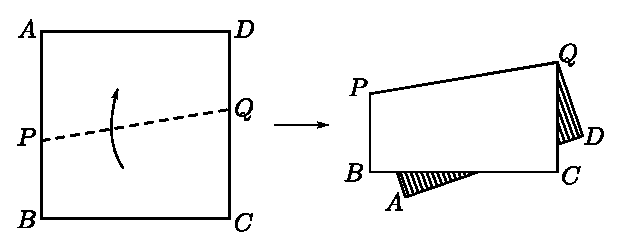
\includegraphics[scale=.98]{src/figure/chap1/fig1-2.eps}
\end{figure}


\item  \textbf{ಪುಸ್ತಕ ಮಡಚುವಿಕೆ : [Book Fold] :} 
ಈ ಮಡಚುವಿಕೆ ತಗ್ಗು ಮಡಚುವಿಕೆಯಂತೆ ಇದೆ. ಈ ಮಡುವಿಕೆ ಪುಸ್ತಕವನ್ನು ಮುಚ್ಚುವ ರೀತಿಯಲ್ಲಿ ಇರುವದರಿಂದ ಇದಕ್ಕೆ ಪುಸ್ತಕ ಮಡಚುವಿಕೆ ಎಂದು ಕರೆಯುತ್ತಾರೆ. 
\begin{figure}[H]
\centering
\includegraphics[scale=.98]{src/figure/chap1/fig1-3.eps}
\end{figure}


\item  \textbf{ಕಪಾಟು ಮಡಚುವಿಕೆ : [Cupboard Fold] :} 
\begin{figure}[H]
\centering
\includegraphics[scale=.98]{src/figure/chap1/fig1-4.eps}
\end{figure}


ಮಧ್ಯದ ದಪ್ಪ ಗೆರೆಯಗುಂಟ ಎರಡು ಬದಿಗಳನ್ನು ಸೇರುವಂತೆ ಎರಡು ಬದಿಗಳನ್ನು ಮಡಚಬೇಕು. ಇದು ಕಪಾಟಿನ ಎರಡು ಬಾಗಿಲಗಳನ್ನು ಮುಚ್ಚುವ ರೀತಿಯಲ್ಲಿ ಇರುವದರಿಂದ ಇದಕ್ಕೆ "ಕಪಾಟು ಮಡಿಕೆ" ಎಂದು ಕರೆಯುತ್ತಾರೆ. 

\item  \textbf{[Pleat Fold] :}
\begin{figure}[H]
\centering
\includegraphics[scale=.98]{src/figure/chap1/fig1-5.eps}
\end{figure}


ಈ ಮಡಚುವಿಕೆಯಲ್ಲಿ ತಗ್ಗು ಮಡಿಕೆ ಮತ್ತು ಉಟ್ಟು ಮಡಿಕೆಗಳ ಜೋಡಣಿ ಇರುತ್ತದೆ. 

\item  \textbf{[Blintz Fold] :}
\begin{figure}[H]
\centering
\includegraphics[scale=.98]{src/figure/chap1/fig1-6.eps}
\end{figure}


ಚೌರ ಪದ 4  ಶೃಂಗ ಬಿಂದುಗಳನ್ನು (ಮೂಲೆಗಳನ್ನು) ಮಧ್ಯ ಬಿಂದುವಿಗೆ ಮುಟ್ಟುದರತೆ ಮಡಚಿದಾಗ [Blintz Bold] ಉಂಟಾಗುತ್ತದೆ. 
 \end{enumerate}


\section*{ಓರಿಗಾಮಿ ವಿಧಾನಗಳು : } ಓರಿಗಾಮಿ ಜ್ಞಾನದಲ್ಲಿ ಆಟದ ಭಾಗವೇ ಹೆಚ್ಚಾಗಿರುವದರಿಂದ ಅದನ್ನೇ ಗಣಿತ ಸಂವಹನೆಗೆ ಉಪಯೋಗಿಸುವುದು ಗಣಿತದ ತಂತ್ರವಾಗಿದೆ. ಗಣಿತದ ಮೂಲ ಸಂಗತಿಗಳನ್ನು ಓರಿಗಾಮಿ ಮೂಲಕ ಪರಿಕಲ್ಪನೆ ಮಾಡಿಕೊಳ್ಳಬೇಕಾದರೆ ಕೆಳಗಿನ ವಿಧಾನಗಳನ್ನು ಬಳಸಲಾಗುತ್ತದೆ. 
\begin{itemize}
\item[(1)] ಕಾಗದವನ್ನು ಮಡಚಿ ತೆರೆಯುವ ವಿಧಾನ.
\item[(2)] ಕಾಗದವನ್ನು ಮಡಚಿ, ಕತ್ತರಿಸಿ ನಂತರ ತೆರೆಯುವ ವಿಧಾನ.
\item[(3)] ಕಾಗದವನ್ನು ಮಡಚಿ ಅಂಟು ಹಚ್ಚುವ ವಿಧಾನ
\item[(4)] ಕಾಗದವನ್ನು ಕತ್ತರಿಸಿ ಬಂದ ತುಂಡುಗಳನ್ನು [ಬಿಲ್ಲೆಗಳು] ಮರುಜೋಡಣೆ ಮಾಡುವ ವಿಧಾನ.
\end{itemize}

\begin{enumerate}
\item  \textbf{ಕಾಗದವನ್ನು ಮಡಚಿ ತೆರೆಯುವ ವಿಧಾನಗಳಿಂದ ಗಣಿತದ ಮೂಲ ಕಲ್ಪನೆಗಳನ್ನು ತಿಳಿದುಕೊಳ್ಳುವದು :} ಒಂದು ಕಾಗದವನ್ನು ಕ್ರಮಬದ್ದವಾಗಿ ಮಡಚಿ ಬಿಚ್ಚುವದರಿಂದ ಉಂಟಾಗುವ ಗೆರೆಗಳನ್ನು ಉಪಯೋಗಿಸಿ ಗಣಿತದ ಮುಖ್ಯ ಸಂಗತಿಗಳನ್ನು ತಿಳಿದುಕೊಳ್ಳಬಹುದು.
\begin{itemize}
\item[(a)]  ಕೋನಮಾಪಕದ ಸಹಾಯವಿಲ್ಲದೆ ನಿರ್ದಿಷ್ಟ ಕೋನಗಳನ್ನು ರಚಿಸುವುದು ಮತ್ತು ಉಪಯೋಗಿಸುವುದು 

\item[(b)] ಚೌರಸ ಆಕರದ ಕಾಗದವನ್ನು ಮಡಚಿ ಹಡಗವನ್ನು ತಯಾರಿಸಿ ಬಿಚ್ಚುವದರಿಂದ ಉಂಟಾಗುವ ಗೆರೆಗಳನ್ನು ಬಳಸಿ. ಪೈಥಾಗೋರಸನ ಪ್ರಮೇಯ, ವಿಸ್ತಾರ  ಪ್ರಮೇಯಗಳನ್ನು ಮತ್ತು ಅಪಲೋನಿಯಸ್ ನ ಪ್ರಮೇಯವನ್ನು ಸಾಧಿಸುವುದು. 

\item[(c)] ತ್ರಿಭುಜ ಆಕಾರದ ಕಾಗದವನ್ನು ನಿರ್ದಿಷ್ಟ ಕ್ರಮದಲ್ಲಿ ಮಡಿಚಿದಾಗ ತ್ರಿಭುಜದ 3 ಕೋನಗಳ ಮೊತ್ತ  180$\circ$ ಸಮವೆಂದು, ನಂತರ ಬಿಚ್ಚಿದಾಗ ತ್ರಿಭುಜದ ವಿಸ್ತೀರ್ಣದ ಸೂತ್ರ $A=bb$ ನ್ನು ಸಾಧಿಸುವುದು. 

\item[(d)]  ಅದೇ ರೀತಿಯಲ್ಲಿ  `y' ದ ಬೆಲೆಯನ್ನು ಸಹ ಕಂಡುಹಿಡಿಯಲು ಬರುತ್ತದೆ. 
\end{itemize}

\item  ಕೋನ ಮಾಪಕದ ಸಹಾಯವಿಲ್ಲದೆ ಕಾಗದವನ್ನು ಮಡಚಿ ನಂತರ ಬಿಚ್ಚಿ. ನಮಗೆ ಬೇಕಾದ ಅಳತೆಯ ಕೋನಗಳನ್ನು ರಚಿಸುವದು. ಈ ಚಟುವಟಿಕೆಗಳನ್ನು ಚೌರಸ ಆಕಾರದ ಕಾಗದವನ್ನು ಉಪಯೋಗಿಸಿ ಕೆಳಗಿನ ಕರಾರಿನಂತೆ ಮಾಡುತ್ತಾರೆ. 
\begin{itemize}
\item[(1)] ಯಾವುದೇ ರೀತಿಯಲ್ಲಿ ಜ್ಯಾಮಿಲೆ ಪೆಟ್ಟಿಗೆಯ ಉಪಕರಣಗಳನ್ನು ಉಪಯೋಗಿಸುವಂತಿಲ್ಲ. ಆದರೆ, ಚಳುವಟಿಕೆ ಮುಗಿದ ನಂತರ ಅಳತೆಮಾಡಿ ಪರೀಕ್ಷಿಸಲು ಕೋನಮಾಪಕವನ್ನು ಉಪಯೋಗಿಸಬಹುದು.

\item[(2)] ಇಲ್ಲಿ ಉಪಯೋಗಿಸುವ ಹಂತಗಳು ಗಣಿತ  ವಿಧಾನಗಳಾಗಿರಬೇಕು.

\item[(3)] ಉಪಯೋಗಿಸುವ ಕಾಗದ ಸರಿಯಾಗಿ ಚೌರಸ ಆಕಾರದಲ್ಲಿರಬೇಕು.

\item[(4)] ಈ ಚಟುವಟಿಕೆಗಳನ್ನು ಕೇವಲ 1 ನಿಮಿಷಕ್ಕಿಂತ ಕಡಿಮೆ ವೇಳೆಯಲ್ಲಿ ಮಾಡಬಹುದು. ಶೇ.  99.9 ರಷ್ಟು ಸರಿ ಬಂದರೆ, ಶೇ.  0.1 ರಷ್ಟು ಮಾತ್ರ ತಪ್ಪಾಗುವ ಸಾಧ್ಯತೆ ಇದೆ. 
\end{itemize}

ಈ ವಿಭಾಗದಲ್ಲಿ 8 ಚಟುವಟಿಕೆಗಳ ಮೂಲಕ ನಿರ್ದಿಷ್ಟ ಅಳತೆಗಳ ಕೋನಗಳನ್ನು ಕಾಗದ ಮಡಚುವದರಿಂದ ರಚನೆ ಮಾಡುವದನ್ನು ವಿವರಿಸಿದೆ. 
\end{enumerate}

\section*{ಚಟುವಟಿಕೆ [1]}
ಚೌರಸ ಕಾಗದವನ್ನು ಮಡಚಿ 90$^\circ$,  45$^\circ$, 22.5$^\circ$, 67.5$^\circ$ ಕೋನಗಳನ್ನು ಕಂಡುಕೊಳ್ಳುವದು. ಒಂದು ಚೌರಸ ಆಕಾರದ ABCD ಕಾಗದವನ್ನು ಮಕ್ಕಳಿಗೆ ತೋರಿಸಿದಾಗ ಎಲ್ಲರೂ ಕಾಗದದ ಮೂಲೆಗಳಲ್ಲಿ (ಶೃಂಗ ಬಿಂದುಗಳಲ್ಲಿ) 90$^\circ$ ಗುರುತಿಸುತ್ತಿರೆ. ಅಂದರೆ, $\angle{A} = 90^\circ$, $\angle{B} = 90^\circ$, $\angle{C} = 90^\circ$, $\angle{D} = 90^\circ$. ಈಗ ಕಾಗದವನ್ನು BD ಕರ್ಣದ ಶುಂಟ ಮಡಿಚಿದಾಗ B ಬಿಂದುವಿನಲ್ಲಿ ಎರಡು ಕೋನಗಳು ಉಂಟಾಗುತ್ತವೆ. ಪ್ರತಿಯೊಂದು  45$^\circ$ ಆಗುತ್ತವೆ. ಅಂದರೆ,  $\angle ABD=45^{\circ}$,  $\angle DBC = 45^\circ$. ಮುಂದುವರಿದು  BC ಬದಿಯನ್ನು $BD$ ಕರ್ಣಕ್ಕೆ ಹೊಂದುವಂತೆ. ಮಡಚಿ ಬಿಟ್ಟಿದಾಗ, ಮತ್ತೆ ಎರಡು ಕೋನಗಳು ದೊರಕುತ್ತವೆ. ಪ್ರತಿಯೊಂದು $22.5{^\circ}$ ಕೋನಗಳು ಉಂಟಾಗುತ್ತವೆ. 

ಅಂದರೆ, $\angle DBE = 22.5$, $\angle EBC = 22.5^\circ$ ಮುಂದುವರಿದು. BC ಬಾಹುವನ್ನು BE ಗೆ ಹೊಂದುವಂತೆ ಮಡಚಿದಾಗ ಮತ್ತೆ ಸಮನಾದ ಎರಡು ಕೋನಗಳು ನಗುತ್ತವೆ. ಅವು ಪ್ರತಿಯೊಂದು 11.25$^\circ$ ಆಗುತ್ತವೆ. 

ಈ ಮಡಿಕೆಯಿಂದ ಇನ್ನು ಬೇರೆ ಬೇರೆ ಕೋನಗಳನ್ನು ಕಂಡು ಕೊಳ್ಳಬಹುದು. ಉದಾಹರಣೆಗಾಗಿ.  $\angle ABE = 67.5^\circ$.
\begin{figure}[H]
\centering
\includegraphics[scale=.98]{src/figure/chap1/fig1-7a.eps}
\end{figure}
\begin{figure}[H]
\centering
\includegraphics[scale=.98]{src/figure/chap1/fig1-7b.eps}
\end{figure}
\begin{figure}[H]
\centering
\includegraphics[scale=.98]{src/figure/chap1/fig1-7c.eps}
\end{figure}
\begin{figure}[H]
\centering
\includegraphics[scale=.98]{src/figure/chap1/fig1-7d.eps}
\end{figure}


\section*{ಚಟುವಟಿಕೆ [2]}  ಆಯತ ಆಕಾರದ ಕಾಗದವನ್ನು ಮಡಚಿ 30$^\circ$ ಮತ್ತು 60$^\circ$ ಕೋನಗಳನ್ನು ರಚಿಸುವದು. 

\textbf{ಮಡಚುವ ಹಂತಗಳು :}
\begin{enumerate}
\item[(1)] ಆಯತ ಆಕಾರದ ಕಾಗದವನ್ನು [ABCD] ತೆಗೆದುಕೊಳ್ಳಬೇಕು.
\begin{figure}[H]
\centering
\includegraphics[scale=.98]{src/figure/chap1/fig1-8a.eps}
\end{figure}

\item[(2)] ಚಿತ್ರದಲ್ಲಿ ತೋರಿಸಿದಂತೆ ಕಾಗದದ `B' ಶೃಂಗಬಿಂದುವಿನಲ್ಲಿ ತ್ರಿಭಾಜಕ ರೇಖೆ  (BE) ಉಂಟಾಗುವಂತೆ BC ಬದಿಯನ್ನು ಮಡಚಿಬೇಕು.
\begin{figure}[H]
\centering
\includegraphics[scale=.98]{src/figure/chap1/fig1-8b.eps}
\end{figure}

\item[(3)] ಚಿತ್ರದಲ್ಲಿ ತೋರಿಸಿದಂತೆ  BC ಗೆ ಹೊಂದುವಂತೆ.  AB ಬದಿಯನ್ನು ಮಡಚಬೇಕು.  ಆಗ ಶೃಂಗಬಿಂದು `A' ಇದು  F ಬಂದುವಿನಲ್ಲಿ ಸೇರುತ್ತದೆ. 
\begin{figure}[H]
\centering
\includegraphics[scale=.98]{src/figure/chap1/fig1-8c.eps}
\end{figure}

\item[(4)] ಮಡಿಕೆಯನ್ನು ಬಿಚ್ಚಿದಾಗ ಚಿತ್ರದಲ್ಲಿ ತೋರಿಸಿದಂತೆ B ಶೃಂಗಬಿಂದುವಿನಲ್ಲಿ ಸಮನಾದ  3 ಕೋನಗಳು ಉಂಟಾಗುತ್ತದೆ. ಪ್ರತಿಯೊಂದು 30$^\circ$ ಗೆ ಸಮವಿರುತ್ತದೆ. ಈ ಮಡಿಕೆಯಿಂದ 30$^\circ$ ಮತ್ತು 60$^\circ$ ಕೋನಗಳನ್ನು ಪಡೆಯಬಹುದು. 
\begin{figure}[H]
\centering
\includegraphics[scale=.98]{src/figure/chap1/fig1-8d.eps}
\end{figure}
\end{enumerate}

\section*{ಚಟುವಟಿಕೆ [3]} ಆಯತ ಆಕಾರದ ಕಾಗದ ಮಡಚಿ 60$^\circ$ ಕೋನವನ್ನು ರಚಿಸುವದು. 

\textbf{ಮಡಚುವ ಹಂತಗಳು :}
\begin{enumerate}
\item[(1)] ಒಂದು ಆಯತಾಕಾರದ ಕಾಗದವನ್ನು [ABCD] ತೆಗೆದುಕೊಂಡ BC ಬಾಹುವಿನ ಮೇಲೆ ಮಧ್ಯದಲ್ಲಿ `O' ಬಿಂದುವನ್ನು ಗುರುತಿಸಿಕೊಳ್ಳಬೇಕು. 
\begin{figure}[H]
\centering
\includegraphics[scale=.98]{src/figure/chap1/fig1-9a.eps}
\end{figure}

\item[(2)] ಚಿತ್ರದಲ್ಲಿ ತೋರಿಸಿದಂತೆ  `O' ಬಿಂದುವಿನಲ್ಲಿ ತ್ರಿಭಾಜಕ ರೇಖೆ (Ox) ಉಂಟಾಗುವಂತೆ. CD ಬದಿಯನ್ನು ಮಡಚಬೇಕು.  
\begin{figure}[H]
\centering
\includegraphics[scale=.98]{src/figure/chap1/fig1-9b.eps}
\end{figure}

\item[(3)] ಅದರಂತೆ OY ರೇಖೆಯಗುಂಟು AB ಬದಿಯನು ಮಡಚಬೇಕು. 
\begin{figure}[H]
\centering
\includegraphics[scale=.98]{src/figure/chap1/fig1-9c.eps}
\end{figure}

\item[(4)] ಮಡಚದ ಕಾಗದವನ್ನು ಬಚ್ಚಿದಾಗ  ಚಿತ್ರದಲ್ಲಿ ತೋರಿಸಿದಂತೆ. `O' ಬಿಂದುವಿನಲ್ಲಿ ಸಮನಾದ 3 ಕೋನಗಳು ಉಂಟಾಗುತ್ತವೆ. ಆಗ ಪ್ರತಿಯೊಂದು ಕೋನವು 60$^\circ$ ಆಗುತ್ತದೆ. ಈ ಮಡಿಕೆಯಿಂದ 60$^\circ$ ಮತ್ತು 120$^\circ$ ಕೋನಗಳನ್ನೂ ರಚಿಸಬಹುದು. 
\begin{figure}[H]
\centering
\includegraphics[scale=.98]{src/figure/chap1/fig1-9d.eps}
\end{figure}
\end{enumerate}

\section*{ಚಟುವಟಿಕೆ [4]} ಚೌರಸ ಆಕಾರದ ಕಾಗದದಿಂದ ನವಿಲನ್ನು ತಯಾರಿಸುವ ಮೊದಲಿನ ಕೆಲವು ಮಡಿಕೆಗಳಿಂದ ಉಂಟಾಗುವ ಗೆರೆಗಳಿಂದ ನಿರ್ದಿಷ್ಟ ಅಳತೆಯ ಕೋನಗಳನ್ನು ರಚಿಸುವದು. 

\noindent
\textbf{ಮಡಚುವ ಹಂತಗಳು :}
\begin{itemize}
\item[(1)] ಚೌರಸ ಆಕಾರದ ಕಾಗದವನ್ನು [ABCD] ತೆರೆದುಕೊಂಡು BD ಕರ್ಣದ ಗುಂಟ ಮಡಚಿ ನಂತರ ತೆರೆಯಬೇಕು. 

[A ಮತ್ತು C ಶೃಂಗಗಳನ್ನು ಸೇರಿಸಿ ಮಡಚಬೇಕು.]
\begin{figure}[H]
\centering
\includegraphics[scale=.98]{src/figure/chap1/fig1-10a.eps}
\end{figure}

\item[(2)] ಚಿತ್ರದಲ್ಲಿ ತೋರಿಸಿದಂತೆ ಕಾಗದದ A ಮತ್ತು  B ಶೃಂಗಗಳನ್ನು ಹಾಗೂ  C ಯ D ಶೃಂಗಗಳನ್ನು ಸೇರಿಸಿ ಮಡಚಿ ನಂತರ ಬಿಚ್ಚಬೇಕು. ಆಗ PQ ರೇಖೆ ದೊರಕುತ್ತದೆ. 
\begin{figure}[H]
\centering
\includegraphics[scale=.98]{src/figure/chap1/fig1-10b.eps}
\end{figure}

\item[(3)] ಚಿತ್ರದಲ್ಲಿ ತೋರಿಸಿದಂತೆ  `A' ಶೃಂಗಬಿಂದುವನ್ನು PQ ರೇಖೆಯ ಮೇಲೆ ಬರುವಂತೆ.  AB ಬದಿಯನ್ನು ಮಡಚಬೇಕು.  A ಶೃಂಗಬಿಂದು  PQ ರೇಖೆಯನ್ನು ಸಂಧಿಸುವ ಬಿಂದು   `R' ಇರಲಿ. 
\begin{figure}[H]
\centering
\includegraphics[scale=.98]{src/figure/chap1/fig1-10c.eps}
\end{figure}

\item[(4)] ಈಗ BC ಬದಿಯನ್ನು AB ಬದಿಗೆ ಹೊಂದುವಂತೆ ಮಡಚಬೇಕು. 
\begin{figure}[H]
\centering
\includegraphics[scale=.98]{src/figure/chap1/fig1-10d.eps}
\end{figure}

\item[(5)] ನಂತರ BD ಕರ್ಣರೇಖೆಯ ಗುಂಟ ಮಡಚಬೇಕು. ಮುಂದೆ ಈ ಮಡಿಕೆಯಿಂದ ಮುಂದೆ ನವೀಲಿನ ಮಾದರಿಯನ್ನು ರಚನೆ. ಮಾಡಬಹುದು. 
\begin{figure}[H]
\centering
\includegraphics[scale=.98]{src/figure/chap1/fig1-10e.eps}
\end{figure}

\item[(6)] ಮಡಚಿದ ಮಾದರಿಯನ್ನು ಪೂರ್ಣವಾಗಿ ಬಿಚ್ಚಿದಾಗ ಚಿತ್ರದಲ್ಲಿ ತೋರಿಸಿದಂತ ಅನೇಕ ರೇಖೆಗಳು [Bx, By, BD, BZ ಮತ್ತು  BW] ಉಂಟಾಗುತ್ತವೆ. ಈ ಗೆರೆಗಳಿಂದ `B' ಬಿಂದುವಿನಲ್ಲಿ ಕೋನಗಳು ಉಂಟಾಗುತ್ತವೆ. ಚಿತ್ರದಲ್ಲಿ 6 ಕೋನಗಳು ಉಂಟಾಗುತ್ತವೆ. ಪ್ರತಿಯೊಂದು ಕೋನವು  15$^\circ$ ಅಳತೆಯ ಕೋನವಾಗಿರುತ್ತದೆ. ಅಂದರೆ. 
\begin{tabbing}
\= \quad \quad \= $\angle  ABW$ \= = \= 15$^\circ$\\
\> \> $\angle WBZ$ \> = \> 15$^\circ$\\
\> \> $\angle  ZBD$ \> = \> 15$^\circ$\\
\> \> $\angle  DBY$ \> = \> 15$^\circ$\\
\> \> $\angle  YBX$ \> = \> 15$^\circ$ \\
ಮತ್ತು \> \> $\angle  XBC$ \> = \> 15$^\circ$
\end{tabbing}
\begin{figure}[H]
\centering
\includegraphics[scale=.98]{src/figure/chap1/fig1-10f.eps}
\end{figure}
\end{itemize}

ಈ ರೀತಿಯ ಮಡಕೆಯಿಂದ ನಾವು $15^\circ$, $30^\circ$, $45^\circ$, $60^\circ$, $75^\circ$, $90^\circ$ ಕೋನಗಳನ್ನು ಪಡೆಯುತ್ತೇನೆ. 

\section*{ಚಟುವಟಿಕೆ [5]} 
ಒಂದು ಚೌರಸ ಆಕಾರದ ಕಾಗದವನ್ನು ಮಡಚಿ $127^\circ.57'$ ಕೋನವನ್ನು ರಚಿಸಲು ಬರುತ್ತದೆ. 

\medskip
\noindent
\textbf{ರಚಿಸುವ ಹಂತಗಳು :}
\begin{enumerate}
\item ABCD ಚೌಕಾಕಾರಾ ಕಾಗದ ತೆರೆದುಕೊಂಡು  AB ಮತ್ತು CD  ಶೃಂಗಗಳನ್ನು ಸೇರಿಸಿ ಮಡಚಿ ಅಡ್ಡರೇಖೆ PQ ವನ್ನು ಗುರುತಿಸಬೇಕು.
\begin{figure}[H]
\centering
\includegraphics[scale=.98]{src/figure/chap1/fig1-11a.eps}
\end{figure}

\item ಕಾಗದಾನ್ನು PQ ಅಡ್ಡ ರೇಖೆಯ ಗುಂಟ ಮಡಬಬೇಕು.  
\begin{figure}[H]
\centering
\includegraphics[scale=.98]{src/figure/chap1/fig1-11b.eps}
\end{figure}

\item ಚಿತ್ರದಲ್ಲಿ ತೋರಿಸಿದಂತೆ. D ಶೃಂಗವನ್ನು AQ ಗುಂಟಮಡಚಬೇಕು ಆಗ  $\angle POD$ ಉಂಟಾಗುವದು. ಅದು ಸರಿಯಾಗಿ $127^\circ.57'$ ಆಗುತ್ತದೆ. 

ಅಂದರೆ, $\angle POD = 127^\circ.57'$ ಆಗುವದು. ಈ ಮಡಿಕೆಯನ್ನು ಉಪಯೋಗಿಸಿಕೊಂಡು ನಾವು ಕೋನಮಾಪಕ ವಿಲ್ಲದೇ ಸಮ ಸಪ್ತ ಬಹುಭುಜಾಕೃತಿಯನ್ನು ರಚಿಸಲು ಬರುತ್ತದೆ. ಇಲ್ಲಿಯವರೆಗೆ ಸುಮಾರು 23 ಪರಿಪೂರ್ಣ ಸಂಖ್ಯೆಗಳನ್ನು ಕಂಡುಹಿಡಿದಿದ್ದಾರೆ. ಅವೆಲ್ಲವೂ ಸಮಸಂಖ್ಯೆಗಳಾಗಿರುತ್ತವೆ.
\begin{figure}[H]
\centering
\includegraphics[scale=.98]{src/figure/chap1/fig1-11c.eps}
\end{figure}
\end{enumerate}

\section*{ಚಟುವಟಿಕೆ [6]}
$10^\circ$ ಕೋನವನ್ನು ರಚಿಸುವದು. ಸುಮಾರು $[16 \times 16]$ ಸೆಂ.ಮಿ. ಅಥವಾ  $[6 \times 6]$ ಅಂಗುಲ ಅಳತೆಯ ಚೌರಸ ಆಕಾರದ ಕಾಗದದಿಂದ ಮಡಚಿ ಮಾಡುತ್ತಾರೆ. 

\medskip
\noindent
\textbf{ಮಡಚುವ ಹಂತಗಳು :}
\begin{enumerate}
\item ಚೌರಸ ಆಕಾರದ ಕಾಗದವನ್ನು [ABCD] ತೆರೆದುಕೊಂಡು ಅದನ್ನು ಮಡಚಿ AC ಕರ್ಣವನ್ನು ಗುರುತಿಸಿಕೊಳ್ಳಬೇಕು. 
\begin{figure}[H]
\centering
\includegraphics[scale=.98]{src/figure/chap1/fig1-12a.eps}
\end{figure}

\item AC ಕರ್ಣದ ಮಧ್ಯಬಿಂದು [x]ವನ್ನು ಮಡಚಿ ಕಂಡುಕೊಳ್ಳಬೇಕು. ಅದರಂತೆ  xc ಮಧ್ಯಬಿಂದುವನ್ನು  [y] ಹಾಗೂ  yc ಯ ಮಧ್ಯಬಿಂದುವನ್ನು ಕಾಗದ ಮಡಚಿ ಕಂಡುಕೊಳ್ಳಬೇಕು. 
\begin{figure}[H]
\centering
\includegraphics[scale=.98]{src/figure/chap1/fig1-12b.eps}
\end{figure}

\item ಚಿತ್ರದಲ್ಲಿ ತೋರಿಸಿದಂತೆ zC=wC ಆಗುವಂತೆ. CD ಬಾಹುವಿನ ಮೇಲೆ  `w' ಬಿಂದುವನ್ನು ಗುರುತಿಸಿ ನಂತರ Bw ವನ್ನು ಸೇರಿಸಬೇಕು. ಆಗ ಉಂಟಾಗುವ. $\angle WBC = 10^\circ$ ಆಗುತ್ತದೆ. 
\begin{figure}[H]
\centering
\includegraphics[scale=.98]{src/figure/chap1/fig1-12c.eps}
\end{figure}
\end{enumerate}

\section*{ಚಟುವಟಿಕೆ [7]}  6 ನೇ ಚಟುವಟಿಕೆಯ ಮಡಚುವಿಕೆಯನ್ನು ಮುಂದುವರಸಿ, 10$^\circ$ ಕೋನಕ್ಕೆ ಸಂಬಂಧಿಸಿದ ಅನೇಕ ಸಂಗತಿಗಳನ್ನು ಕಂಡುಕೊಳ್ಳಬಹುದು. 

\medskip
\noindent
\textbf{ಮಡಚುವಿಕೆಯ ಹಂತಗಳು :}
\begin{enumerate}
\item[(1)] ಚಟುವಟಿಕೆ - 6 ರಲ್ಲಿ ತೋರಿಸಿದಂತೆ ಚೌರಸ ಆಕಾರದ ಕಾಗದವನ್ನು ಮಡಚಿ $\angle PBC = 10^\circ$ ಯನ್ನು ರಚಿಸಬೇಕು.
\begin{figure}[H]
\centering
\includegraphics[scale=.98]{src/figure/chap1/fig1-13a.eps}
\end{figure}

\item[(2)] ಚಿತ್ರದಲ್ಲಿ ತೋರಿಸಿದಂತೆ, D ಬಿಂದು BP ರೇಖೆಗೆ ಹೊಂದುವಂತೆ ಮಡಚಬೇಕು. ಆಗ ಅನೇಕ ಅಳತೆಯ ಕೋನಗಳು ದೊರಕುತ್ತವೆ. 
\begin{figure}[H]
\centering
\includegraphics[scale=.98]{src/figure/chap1/fig1-13b.eps}
\end{figure}
\begin{itemize}
\item[(i)] $\Delta PBC$ ಯಲ್ಲಿ $\angle PBC =  10^\circ$ ಮತ್ತು $\angle C =90^\circ$  $\therefore ~ \angle BPC = 80^\circ$.

\item[(ii)] ಚಿತ್ರದಲ್ಲಿ $\Delta PBC$ ಮತ್ತು $\Delta ABD$ ಇವು ಸರ್ವಸಮ ತ್ರಿಭುಜಗಳು.

$\therefore \angle BAD = 10^\circ$, $\angle ABD = 80^\circ$ ಮತ್ತು $\angle ADB = 90^\circ$.

\item[(iii)] ಚಿತ್ರದಲ್ಲಿ $AB = BP$ \quad $\therefore ~ \angle BPA = \angle BAP = 50^\circ$

\item[(iv)] ಆದ್ದರಿಂದ $\angle DAP = 50^\circ - 10^\circ = 40^\circ$

\item[(v)] ಪೂರಕ ಕೋನಗಳು (i) $\angle DAP + \angle DPA = 40^\circ + 50^\circ \ 90^\circ$

\item[(vi)] ಪರಿಪೂರಕ ಕೋನಗಳು  (i) $\angle BDA + \angle ADP = 50^\circ + 90^\circ = 180^\circ $

\item[(vii)] ತ್ರಿಭುಜದ ಒಂದು ಬಾಹುವನ್ನು ಬೆಳೆಸಿದಾಗ ಉಂಟಾಗುವ ಹೊರ ಕೋನವು ಅಂತರ ವಿರುದ್ಧ ಕೋನಗಳ ಮೊತ್ತಕ್ಕೆ ಸಮವಿದೆ. 

ಚಿತ್ರದಲ್ಲಿ $\angle ADP = \angle ABD + \angle BAD = 80^\circ + 10^\circ = 90^\circ$.
\end{itemize}
\end{enumerate}

\section*{ಚಟುವಟಿಕೆ [8]} $20^\circ$ ಕೋನವನ್ನು ರಚಿಸುವದು. 

ಸುಮಾರು [$10 \times 10$] ಸೆಂ.ಮಿ. ಅಳತೆಯ ಚೌರಸ ಆಕಾರದ ಕಾಗದವನ್ನು ಉಪಯೋಗಿಸಿ ಕೆಳಗಿನಂತೆ ಮಡಚಿ.  20$^\circ$ ಕೋನವನ್ನು ರಚಿಸುತ್ತಾರೆ. 

\medskip
\noindent
\textbf{ಮಡಚುವ ಹಂತಗಳು :}
\begin{enumerate}
\item[(1)] 10 ಸೆಂ.ಮಿ. ಒಂದು ಬಾಹು ಇರುವ ಒಂದು ಚೌರಸ ಆಕಾರದ ಕಾಗದ  [ABCD] ತೆಗೆದುಕೊಂಡು, ಅದರ CD ಬಾಹುವನ್ನು ಮಡಚಿ ಅದರ ಮಧ್ಯಬಿಂದು [M] ವನ್ನು ಮತ್ತು MC ಯ ಮಧ್ಯಬಿಂದು [Y] ಯನ್ನು ಕಂಡುಕೊಳ್ಳಬೇಕು. 
\begin{figure}[H]
\centering
\includegraphics[scale=.98]{src/figure/chap1/fig1-14a.eps}
\end{figure}

\item[(2)] y ಬಿಂದುವಿನಲ್ಲಿ  xy || BC ಆಗುವಂತೆ. ಮಡಚಿ xy ರೇಖೆಯನ್ನು ಗುರುತಿಸಬೇಕು. ಆಗ `x' ಬಿಂದು AB ಬಾಹುವಿನಲ್ಲಿ ಬರುತ್ತದೆ. 
\begin{figure}[H]
\centering
\includegraphics[scale=.98]{src/figure/chap1/fig1-14b.eps}
\end{figure}

\item[(3)] xy ದ ಮಧ್ಯ ಬಿಂದು (z) ನ್ನು ಮಡಚಿ. ಕಂಡುಕೊಳ್ಳಬೇಕು. ನಂತರ zy ದ ಮಧ್ಯಬಿಂದು w ನ್ನು ಕಂಡುಹಿಡಿಯಬೇಕು. ಆಗ wy = $\dfrac{1}{2}$ zy = 2.5 ಮೌನಗಳು. 

\item[(4)] ನಂತರ xw ದ ಮಧ್ಯಬಿಂದು M ನ್ನು ಮಡಚಿಕಂಡುಕೊಳ್ಳಬೇಕು. ಮತ್ತು M y ದ ಮಧ್ಯಬಿಂದು  P ಯನ್ನು ಮಡಚಿ ಕಂಡುಕೊಳ್ಳಬೇಕು.

\item[(5)] ಈಗ BP ಸೇರಿಸಿ PQ $\perp$ BC ಯನ್ನು ಮಡಚಿ ಕಂಡುಹಿಡಿಯಬೇಕು. ಆಗ PQ = 2.5 ಮೌನಗಳು ಹಾಗೂ  $\angle PBQ = 20^\circ$ ಆಗುವದು.  
ಸಮತಲಾಕೃತಿಗಳನ್ನು ಓರಿಗಾಮಿ ವಿಧಾನದಿಂದ ತಯಾರಿಸಿ. ಕಾಗದವನ್ನು ಮಡಚಿ ಕತ್ತರಿಸುವದರಿಂದ ಗಣಿತದ ಸಮತಲಾಕೃತಿಗಳ ಪರಿಕಲ್ಪನೆಗಳನ್ನು ಮಾಡಿಕೊಳ್ಳುವದು. 
\end{enumerate}

\begin{itemize}
\item[(a)] \textbf{ಚೌರಸದ ರಚನೆ:}
\begin{figure}[H]
\centering
\includegraphics[scale=.98]{src/figure/chap1/fig1-15a.eps}
\end{figure}

ಚಿತ್ರದಲ್ಲಿ ತೋರಿಸಿದಂತೆ ABCD ಆಯತ ಆಕಾರದ ಒಂದು ಕಾಗದ ತೆರೆದುಕೊಂಡು, D ಶೃಂಗ ಬಿಂದು AB ಮೇಲೆ ಮುಟ್ಟುವಂತೆ ಮಡಚಿ DE ಗುಂಟ ಕತ್ತರಿಸಿದಾಗ ನಮಗೆ  AFED ಚೌರಸ ದೊರಕುವದು. 

\item[(b)] \textbf{ತ್ರಾಪಿಜ್ಯ ರಚನೆ :}
\begin{figure}[H]
\centering
\includegraphics[scale=.98]{src/figure/chap1/fig1-15b.eps}
\end{figure}

ಚಿತ್ರದಲ್ಲಿ ತೋರಿಸಿದಂತೆ ABCD ಆಯತಾಕಾರದ ಕಾಗದ ತೆರೆದುಕೊಂಡು ಅಡ್ಡವಾಗಿ ಮಡಚಿ, xy ಗುಂಟ ಕತ್ತರಿಸಿದು ಬಿಚ್ಚಿದಾಗ ನಮಗೆ xyzw ತ್ರಾಪಿಜ್ಯ ದೊರಕುವದು. 

\item[(c)] \textbf{ವಜ್ರಾಕೃತಿ ರಚನೆ :}
\begin{figure}[H]
\centering
\includegraphics[scale=.98]{src/figure/chap1/fig1-15c.eps}
\end{figure}

ಚಿತ್ರದಲ್ಲಿ ತೋರಿಸಿದಂತೆ  ABCD ಆಯತ ಆಕಾರದ ಕಾಗದ ತೆಗೆದುಕೊಂಡು ಲಂಬವಾಗಿ ಹಾಗೂ ಅಡ್ಡವಾಗಿ ಮಡಚಿ ಒಂದು ಚಿಕ್ಕ ಆಯತದ ಕರ್ಣದ ಗುಂಟ ಕತ್ತರಿಸಿ ಬಿಚ್ಚಿದರೆ PQRS ವಜ್ರಾಕೃತಿ ದೊರಕುತ್ತದೆ. 

\item[(d)] \textbf{ಸಮದ್ವಿಬಾಹು ತ್ರಿಭುಜ :}
\begin{figure}[H]
\centering
\includegraphics[scale=.98]{src/figure/chap1/fig1-15d.eps}
\end{figure}

ಚಿತ್ರದಲ್ಲಿ ತೋರಿಸಿದಂತೆ, `ABCD' ಆಯತಾಕಾರದ ಕಾಗದ ತೆರೆದುಕೊಂಡು ಮೂಲಕ ಮಡಿಚಿದಾಗ (ಪುಸ್ತಕ ಮಡಿಚಿಕೆ) A ಮತ್ತು D ಹಾಗೂ  B ಮತ್ತು  C ಗಳು ಪರಸ್ಪರ ಸೇರಿಕೊಳ್ಳುತ್ತವೆ. ನಂತರ PB ಗುಂಟ ಕತ್ತರಿಸಿ ಬಿಟ್ಟಿದಾಗ ನಮಗೆ  PBC ಸಮದ್ವಿಬಾಹು ತ್ರಿಭುಜ ದೊರಕುತ್ತದೆ. 


\item[(e)] \textbf{ಸಮಬಾಹು ತ್ರಿಭುಜ : }
\begin{figure}[H]
\centering
\includegraphics[scale=.98]{src/figure/chap1/fig1-15e.eps}
\end{figure}

ಚಿತ್ರದಲ್ಲಿ ತೋರಿಸಿದಂತೆ ABCD ಆಯತಾಕಾರದ ಕಾಗದ ತೆಗೆದುಕೊಂಡು A ಮತ್ತು  D ಶೃಂಗಗಳನ್ನು PR ಮತ್ತು PQ  ಬಾಹುಗಳ ಮೆಲೆ ಬರುವಂತೆ ಮಡಚಿ  PQ, QR ಮತ್ತು PR ಗುಂಟ ಕತ್ತರಿಸಿದಾಗ ನಮಗೆ PQR ಸಮಬಾಹು ತ್ರಿಭುಜ ದೊರಕುತ್ತದೆ. 
\end{itemize}

\medskip
\noindent
\textbf{ಕಾಗದ ಮಡಚಿ ಕತ್ತರಿಸುವದರಿಂದ ಬಹುಭುಜಾಕೃತಿಗಳನ್ನು ರಚಿಸುವದು.}
\begin{itemize}
\item[(a)] \textbf{ಸಮ ಪಂಚಬಹುಭೂಕೃತಿಯನ್ನು ರಚಿಸುವದು.}
\begin{figure}[H]
\centering
\includegraphics[scale=.98]{src/figure/chap1/fig1-16a.eps}
\end{figure}

ಚಿತ್ರದಲ್ಲಿ ತೋರಿಸಿದಂತೆ ಉದ್ದನೆಯ ಒಂದು ಕಾಗದದ ಪಟ್ಟಿಯನ್ನು ತೆರೆದುಕೊಂಡು ಕೈ ಕಟ್ಟುವ ರೀತಿಯಲ್ಲಿ ಒಂದು ಗಂಟನ್ನು ಹಾಕಬೇಕು. ನಂತರ ಗೆರೆಹಾಕಿದ ಭಾಗವನ್ನು ಕತ್ತರಿಸಿದಾಗ ನಮಗೆ,  ABCDE ಒಂದು ಸಮಬಾಹು ಪಂಚಬಹುಭುಜಾಕೃತಿ ದೊರಕುತ್ತದೆ. 

ದೊರಕಿದ ಪಂಚಬಹುಭುಜಾಕೃತಿಯ ಎಲ್ಲ ಬಾಹುಗಳನ್ನು ಅಳೆದಾಗ ಅವು ಪರಸ್ಪರ ಸಮವಿದ್ದದ್ದು ಹಾಗೂ ಪ್ರತಿಯೊಂದು ಕೋನವನ್ನೂ ಕೋನ ಮಾಪಕದ ಸಹಾಯದಿಂದ ಅಳೆದಾಗ ಪ್ರತಿಯೊಂದು ಕೋನವು $108^\circ$ ಗೆ ಸಮವಿದ್ದದ್ದು ಕಂಡುಬರುತ್ತದೆ. 

ಟೈ ಕಟ್ಟುವುದು ಸಾಮಾನ್ಯ ಪದ್ದತಿಯಲ್ಲ - ಗ್ರಾಮೀಣ ವಿದ್ಯಾರ್ಥಿಗಳಿಗೆ ಇದು ಹೆಸರು. ಈಗೆಲ್ಲಾ ಸಿದ್ದ ಟೈ ಬರುವುದರಿಂದ ಗಂಟು ಹಾಕುವುದು ಹೇಗೆಂದು ವಿವರಿಸಬೇಕು. 

\item[(b)] ಆಯಾತ ಆಕಾರದ ಕಾಗದವನ್ನು ಮಡಚಿ "ಸಮ ಷಡ್ಬುಜಾಕೃತಿ"ಯನ್ನು ರಚಿಸುವದು. 

\medskip
\noindent
\textbf{ಮಡಚುವ ವಿಧಾನಗಳು : }

\begin{enumerate}
\item[(1)] ಆಯತ ಆಕಾರದ ಒಂದು ಕಾಗದವನ್ನು [ABCD] ತೆಗೆದುಕೊಳ್ಳಬೇಕು.
\begin{figure}[H]
\centering
\includegraphics[scale=.98]{src/figure/chap1/fig1-16b1.eps}
\end{figure}

\item[(2)] ಚಿತ್ರದಲ್ಲಿ ತೋರಿಸಿದಂತೆ PQ ರೇಖೆಯ ಗುಂಟ A ಮತ್ತು  B ಹಾಗೂ  C ಮತ್ತು  D ಶೃಂಗಗಳು ಸೇರುವ ಹಾಗೆ. ಮಡಚಬೇಕು. ಹಾಗೂ PQ ಬದಿಯ ಮೇಲೆ `O' ಬಿಂದುವನ್ನು ಗುರುತಿಸಬೇಕು.
\begin{figure}[H]
\centering
\includegraphics[scale=.98]{src/figure/chap1/fig1-16b2.eps}
\end{figure}

\item[(3)] ಚಿತ್ರದಲ್ಲಿ ತೋರಿಸಿದಂತೆ  `O' ಬಿಂದುವಿನಲ್ಲಿ ಸಮನಾಗಿ (3 ಭಾಗಗಳಲ್ಲಿ 2 ಭಾಗಗಳು ಮತ್ತು 1 ಭಾಗ) ಉಂಟಾಗುವ ಹಾಗೆ. Q ಶೃಂಗ ಬಿಂದುವನ್ನು ಮಡಚಬೇಕು. ಆಗ ನಮಗೆ R ಮತ್ತು  S ಬಿಂದುಗಳು ದೊರಕುತ್ತವೆ. 
\begin{figure}[H]
\centering
\includegraphics[scale=.98]{src/figure/chap1/fig1-16b3.eps}
\end{figure}

\item[(4)] ಅದರಂತೆ. `P' ಶೃಂಗ ಬಿಂದುವನ್ನು OQ ಗೆ ಹೊಂದುವಂತೆ ಮಡಚಬೇಕು. ಹಾಗೂ RS ರೇಖೆ ರಚಿಸಿ ಅದರ ಗುಂಟ ಕತ್ತರಿಸಬೇಕು. 
\begin{figure}[H]
\centering
\includegraphics[scale=.98]{src/figure/chap1/fig1-16b4.eps}
\end{figure}

\item[(5)] ಮಡಕೆಯನ್ನು ಬಿಟ್ಟಿದಾಗ ನಮಗೆ ಸಮ ಷಡ್ಬುಜಾಕೃತಿ ದೊರೆಕುತ್ತದೆ. ಅದರಲ್ಲಿ 6 ಸಮಬಾಹು ತ್ರಿಭುಜಗಳು ದೊರಕುತ್ತಿವೆ. 
\begin{figure}[H]
\centering
\includegraphics[scale=.98]{src/figure/chap1/fig1-16b5.eps}
\end{figure}
\end{enumerate}

\item[(c)]  \textbf{ಸಮಸಪ್ತ ಬಹುಭುಜಕೃತಿಯ ರಚನೆ :} ಸಮಸಪ್ತ ಬಹುಭುಜಾಕೃತಿಯನ್ನು ಜ್ಯಾಮಿತಿ ಪೆಟ್ಟಿಗೆ ಇದ್ದರೂ ಸಹ ರಚಿಸುವದು ಸುಲಭವಲ್ಲ. ಯಾಕಂದರೆ ಅದರ ಪ್ರತಿಯೊಂದು ಒಳಕೋನದ ಅಳತೆ $127^\circ.57'$ ಇರುತ್ತದೆ. ಆದರೆ ಕಾಗದ ಮಡಚುವದರಿಂದ ಮೊದಲು $127^\circ.57'$ ಕೋನ ರಚಿಸಿ ಅದರ ಸಹಾಯದಿಂದ ಸಮಸಪ್ತ ಬಹು ಭುಜಾಕೃತಿಯನ್ನು ರಚಿಸಬಹುದು. 

\medskip
\noindent
\textbf{$127^\circ.57'$ ಕೋನವನ್ನು ರಚಿಸುವದು : ಹಂತಗಳು :}
\begin{enumerate}
\item[(1)] ABCD ಚೌರಸ ಆಕಾರದ ಕಾಗದ ತೆಗೆದುಕೊಂಡು. B ಮತ್ತು C ಶೃಂಗಗಳು A ಮತ್ತು D ಬಿಂದುಗಳಿಗೆ ಸೇರುವಂತೆ ಮಾಡಬೇಕು.
 \begin{figure}[H]
\centering
\includegraphics[scale=.98]{src/figure/chap1/fig1-16c1.eps}
\end{figure}

\item[(2)] ಮಡಚಿದ ಭಾಗ PQ ಇರಲಿ, ನಂತರ C ಮತ್ತು D ಶೃಂಗಬಿಂದುಗಳನ್ನು AQ ಕರ್ಣದ ಗುಂಟ ಮಡಚಬೇಕು. ಆಗ AD ಭಾಗವು  PQ ಕರ್ಣದ ಗುಂಟ ಮಡಚಿದಾಗ, ಅದು `O' ಬಿಂದುವಿನಲ್ಲಿ ಛೇದಿಸುತ್ತದೆ. 
 
\item[(3)] ಈಗ ಉಂಟಾಗುವ $\angle POD = 127^\circ.57'$ ಆಗುವದು. 
\end{enumerate}

\medskip
\noindent
\textbf{ಸಮಸಪ್ತ ಬಹುಭುಜಾಕೃತಿಯನ್ನು ರಚಿಸುವದು.}

$\angle POD =127^\circ .57'$ ಇದನ್ನು ಉಪಯೋಗಿಸಿ ಕೆಳಗಿನಂತೆ ಸಮಸಪ್ತಬಹುಭುಜಾಕೃತಿಯನ್ನು ರಚಿಸುತ್ತಾರೆ. 

ಅನುಕೂಲ ಅಳತೆಯ EF ರೇಖೆಯನ್ನು ಎಳೆದು ಮಡಚಿದ ಕೋನ $\angle POD$ ಉಪಯೋಗಿಸಿ F ಬಿಂದುವಿನಲ್ಲಿ  $127^\circ .57'$ ಕೋನವನ್ನು ಮಾಡಿ  EF = FG ಆಗುವಂತೆ G ಬಿಂದುವನ್ನು ಗುರುತಿಸಬೇಕು.  ಇದೇ ರೀತಿಯಲ್ಲಿ G ಬಿಂದುವಿನಲ್ಲಿ $127^\circ .57'$ ಕೋನ ಮಾಡಬೇಕು. ಹಾಗಿಯೆ ಮುಂದುವರಿಸಿ EFGHIJK ಸಮ ಸಪ್ತ ಬಹುಭುಜಾಕೃತಿಯನ್ನು ರಚಿಸಬೇಕು.
\begin{figure}[H]
\centering
\includegraphics[scale=.98]{src/figure/chap1/fig1-16c2.eps}\\
\text{ಸಮಸಪ್ತ ಬಹುಭುಜಾಕೃತಿ}
\end{figure}
 
 
\item[(d)] \textbf{ಸಮ ಅಷ್ಟಭುಜಾಕೃತಿಯ ರಚನೆ :} ಒಂದು ಚೌರಸ ಆಕಾರದ ಕಾಗದರಿಂದ ಮಡುಚುವಿಕೆಯಿಂದ ಹಾಗೂ ಕತ್ತರಿಸುವಿಕೆಯಿಂದ ಸಮ ಅಷ್ಟಭುಜಾಕೃತಿಯನ್ನು ರಚಿಸಲು ಬರುತ್ತದೆ. 

\noindent
\textbf{ಮಡಚುವ ವಿಧಾನದ ಹಂತಗಳು :}
\begin{figure}[H]
\centering
\includegraphics[scale=.98]{src/figure/chap1/fig1-16d1.eps}
\end{figure}
 
 ಚಿತ್ರದಲ್ಲಿ ತೋರಿಸಿದಂತೆ, 4 ಎಸಳುಗಳಲ್ಲಿ ಒಂದನ್ನು ಮಡಚಿ ನಂತರ ಉಳಿದ 3 ಎಸಳನ್ನು ಅದೇ ರೀತಿಗಳಲ್ಲಿ ಮಡಚಬೇಕು. ನಂತರ ಪೂರ್ಣ ಬಿಚ್ಚಿದಾಗ ನಮಗೆ ಅನೇಕ ಗೆರೆಗಳನ್ನು ಹೊಂದಿರುವ ಕಾಗದ ದೊರಕುತ್ತದೆ. ನಂತರ ಗೆರೆಹಾಕಿದ ಗುಂಟ ಕತ್ತರಿಸಿದಾಗ ನಮಗೆ ಸಮ ಅಷ್ಟ ಬಹುಭುಜಾಕೃತಿ ದೊರಕುತ್ತದೆ. 
 \begin{figure}[H]
\centering
\includegraphics[scale=.98]{src/figure/chap1/fig1-16d2.eps}
\end{figure}

ಕಾಗದ ಹಡಗವನ್ನು ಮಡಚಿ ತಯಾರಿಸಿ ನಂತರ ಬಿಟ್ಟ. ಅದರಿಂದ ಪೈಥಾರೋರಾಸ್ ನ ಪ್ರಮೇಯ ಮತ್ತು ಅದರ ವಿಸ್ತಾರ ಪ್ರಮೇಯಗಳು ಮತ್ತು ಅಪಲೋನಿಯಸ್ ನ ಪ್ರಮೇಯಗಳನ್ನು ಸಾಧಿಸುವದು. 

\noindent
\medskip
\textbf{ಒಂದು ಚೌಕ ಕಾಗದದಿಂದ ಹಡಗವನ್ನು ರಚಿಸುವದು:}
\begin{figure}[H]
\centering
\includegraphics[scale=.98]{src/figure/chap1/fig1-17a.eps}
\end{figure}
\begin{figure}[H]
\centering
\includegraphics[scale=.98]{src/figure/chap1/fig1-17b.eps}
\end{figure}
\begin{figure}[H]
\centering
\includegraphics[scale=.98]{src/figure/chap1/fig1-17c.eps}
\end{figure}

ಮೇಲಿನಂತೆ ಕಾಗದವನ್ನು 9 ಹಂತಗಳಲ್ಲಿ ಮಡಚಿ ಬಿಚ್ಚಿದಾಗ ಕಾಗದದಲ್ಲಿ ಗೆರೆಗಳ ಮೂಲಕ 32 ಲಂಬಕೋನ ತ್ರಿಭುಜಗಳು ಉಂಟಾಗುತ್ತವೆ. ಈ ತ್ರಿಭುಜಗಳಿಂದ ಪೈಥಾಗೋರಾಸನ್ ಪ್ರಮೇಯ ಮತ್ತು ವಿಸ್ತಾರ ಪ್ರಮೇಯಗಳನ್ನು ಹಾಗೂ ಅಪಲೋನಿಯಸ್ ನ ಪ್ರಮೇಯಗಳನ್ನು ಮುಂದೆ ತೋರಿಸಿದಂತೆ ಸಾಧಿಸಬಹುದು. 

ಕಾಗದ ಹಡಗವನ್ನು ರಚಿಸಿ ಬಿಚ್ಚಿದಾಗ ಉಂಟಾಗುವ ಗೆರೆಗಳ ಮೂಲಕ ಪೈಥಾಗೋರಾಸ್ ನ ಪ್ರಮೇಯವನ್ನು ಸಾಧಿಸುವುದು. 

\noindent
\medskip
\textbf{ಪೈಥಾಗೋರಾಸ್ ನ ಪ್ರಮೇಯ :} ಲಂಬಕೋನ ತ್ರಿಭುಜದಲ್ಲಿ ಕರ್ಣದ ವರ್ಗವು ಉಳಿದ ಎರಡು ಬಾಹುಗಳ ವರ್ಗಗಳ ಮೊತ್ತಕ್ಕೆ ಸಮವಿರುತ್ತದೆ. 
\begin{figure}[H]
\centering
\includegraphics[scale=.98]{src/figure/chap1/fig1-17d.eps}
\end{figure}

ಚಿತ್ರದಲ್ಲಿ $\angle ABC = 90^\circ$ $\therefore ~ AC^2 =  AB^2 +  BC^2 $

\medskip
\noindent
\textbf{ಈಗ ಪೈಥಾಗೋರಾಸ್ ನ ಪ್ರಮೇಯವನ್ನು ಸಾಧಿಸುವದು :} ಚಿತ್ರದಲ್ಲಿ ತೋರಿಸಿದಂತೆ ಬಿಟ್ಟಿದ ಕಾಗದ ಮೇಲೆ ಉಂಟಾಗುವ 32 ಲಂಬಕೋನ ತ್ರಿಭುಜಗಳಲ್ಲಿ ABC ಎಂಬ ಒಂದು ಲಂಬಕೋನ ತ್ರಿಭುಜವನ್ನು ಗುರುತಿಸಬೇಕು. ನಂತರ ಆ ತ್ರಿಭುಜದ 3 ಬಾಹುಗಳ ಮೇಲೆ ಉಂಟಾಗುವ ಲಂಬಕೋನ ತ್ರಿಭುಜಗಳನ್ನು ಗುರುತಿಸಬೇಕು ಅವು ಕೆಳಗಿನಂತೆ ಇವೆ. 
\begin{figure}[H]
\centering
\includegraphics[scale=.98]{src/figure/chap1/fig1-17e.eps}
\end{figure} 

$AB$ ಬಾಹುವಿನ ಮೇಲಿನ ತ್ರಿಭುಜಗಳು = 2 

$BC$ ಬಾಹುವಿನ ಮೇಲಿನ ತ್ರಿಭುಜಗಳು  = 2

$AC$ ಕರ್ಣದ ಮೇಲಿನ ತ್ರಿಭುಜಗಳು = 4

ಅಂದರೆ  $AB$ಯ ವರ್ಗ $AB^2 =2 $ ತ್ರಿಭುಜಗಳು 

$BC$ ಯ ವರ್ಗ $BC^2 = 2 $  ತ್ರಿಭುಜಗಳು

$AC$ ಯ ವರ್ಗ $AC^2 = 4$  ತ್ರಿಭುಜಗಳು

$\therefore ~ 4 = 2+2$ \quad $\therefore ~ AC^2 = AB^2 + BC^2$
\end{itemize}

\medskip
\noindent
\textbf{ಪೈಥಾಗೋರಾಸ್ ನ ವಿಸ್ತಾರ ಪ್ರಮೇಯಗಳನ್ನು ಸಾಧಿಸುವದು.}

\medskip
\noindent
\textbf{ವಿಸ್ತಾರ ಪ್ರಮೇಯ : 1} ವಿಶಾಲಕೋನ ತ್ರಿಭುಜದಲ್ಲಿ ಲಘುಕೋನಕ್ಕೆ ಎದುರಾಗಿರುವ ಬಾಹುವಿನ ವರ್ಗವು ಉಳಿದ ಎರಡು ಬಾಹುಗಳ ವರ್ಗಗಳ ಮೊತ್ತಕ್ಕಿಂತ ಕಡಿಮೆ ಇರುತ್ತದೆ. ಈ ವ್ಯತ್ಯಾಸವು ಎರಡು ಬಾಹುಗಳಲ್ಲಿ ಒಂದು ಬಾಹು ಮತ್ತು ಅದರ ಮೇಲೆ ಮತ್ತೊಂದರ ಪ್ರಕ್ಷೇಪ ಇವುಗಳ ಗುಣಲಭ್ದದ ಎರಡು ಪಟ್ಟು ಇರುತ್ತದೆ. 

\medskip
\noindent
\textbf{ಸಾಧಾನೆ :} ಮಡಚಿಬಚ್ಚಿದ ಕಾಗದಲ್ಲಿ ಗೆರೆಗಳಗುಂಟ ಒಂದು ABC ವಿಶಾಲಕೋನ. ತ್ರಿಭುಜವನ್ನು ರಚಿಸಬೇಕು. ಅದರಲ್ಲಿ $\angle ACB$ ಒಂದು ಲಘುಕೋನವಾಗಿರಲಿ. ಈಗ ಅದರ ಬಾಹುಗಳ ಮೇಲೆ ಉಂಟಾಗುವ ಲಂಬಕೋನ ತ್ರಿಭುಜಗಳನ್ನು ಏಣಿಕೆ ಮಾಡಿ ಹಚ್ಚಬೇಕು. 
\begin{figure}[H]
\centering
\includegraphics[scale=.98]{src/figure/chap1/fig1-17f.eps}
\end{figure} 

ಅಂದರೆ BC ಬಾಹುವಿನ ಮೇಲೆ = 2  ತ್ರಿಭುಜಗಳು 

AB ಬಾಹುವಿನ ಮೇಲೆ = 4 ಲಂಬಕೋನ ತ್ರಿಭುಜಗಳು. 

ಮತ್ತು AC ಯ ಮೇಲೆ ಒಂದ ಚೌರಸನ್ನು ರಚಿಸಿದರೆ. ಕೆಲವೊಂದ ಲಂಬಕೋನಗಳು ಪೂರ್ಣವಾಗಿ ಮತ್ತು ಕೆಲವೊಂದು ಅಪೂರ್ಣವಾಗಿ ಬರುತ್ತವೆ. ಅಪೂರ್ಣವಾಗಿ ಬಂದ ಲಂಬಕೋನ ತ್ರಿಭುಜಗಳನ್ನು ಚಿತ್ರದಲ್ಲಿ ತೋರಿಸಿದಂತೆ ಸರಿದೂಗಿಸಿದಾಗ ಉಂಟಾಗುವ ಲಂಬಕೋನಗಳ ಸಂಖ್ಯೆ = 4 ಆಗುವದು. 

\begin{tabbing}
 ಚಿತ್ರದಲ್ಲಿ \quad 	\= ~~~ 			$AB^2$~~ \= =  \= $BC^2 + AC^2 - 2 BC \times DC$\\
  $\therefore$ \> \quad $4$ \>  = \> $2+10- \times 1 \times 4$\\
   $\therefore$ \> \quad  $4$ \> = \> $12-8$\\
   $\therefore$ \> \quad $4 $ \> = \> $4$ \\
 $\therefore $ \>  $AB^2$~ \> = \> $BC^2 + AC^2 - 2 BC \times DC$
\end{tabbing}

\medskip
\noindent
\textbf{ವಿಸ್ತಾರ ಪ್ರಮೇಯ : 2}
ತ್ರಿಭುಜದಲ್ಲಿ ವಿಶಾಲಕೋನಕ್ಕೆ ಎದುರಾಗಿರುವ ಬಾಹುವಿನ ವರ್ಗವು ಉಳಿದ ಎರಡು ಬಾಹುಗಳು ವರ್ಗಗಳ ಮೊತ್ತಕ್ಕಿಂತ ಹೆಚ್ಚು. ಇರುತ್ತದೆ. ಈ ವ್ಯತ್ಯಾಸವು ಆ ಎರಡು ಬಾಹುಗಳಲ್ಲಿ ಒಂದು ಬಾಹು ಮತ್ತು ಅವುಗಳ ಮೇಲೆ ಮತ್ತೊಂದರ ಪ್ರಕ್ಷೇಪ ಇವುಗಳ ಗುಣಲಭ್ದದ ಎರಡು ಪಟ್ಟು ಇರುತ್ತದೆ. 
\begin{figure}[H]
\centering
\includegraphics[scale=.98]{src/figure/chap1/fig1-17g.eps}
\end{figure}

ಚಿತ್ರದಲ್ಲಿ ತೋರಿಸಿದಂತೆ ಮಡಚಿಬಿಟ್ಟಿದ ಕಾಗದಲ್ಲಿಯ ಗೆರೆಗಳನ್ನು ಉಪಯೋಗಿಸಿ ABC ಒಂದು ವಿಶಾಲಕೋನ ತ್ರಿಭುಜವನ್ನು ಗುರುತಿಸಬೇಕು. ಇದರಲ್ಲಿ LABC ಒಂದು ವಿಶಾಲಕೋನವಾಗಿದೆ. ಮತ್ತು ಈ ತ್ರಿಭುಜದ 3 ಬಾಹುಗಳ ಮೇಲಿನ ತ್ರಿಭುಜಗಳನ್ನು ಎಣಿಕೆಮಾಡಿ ಕೆಳಗಿನಂತೆ ಹೆಚ್ಚಬೇಕು.

BC ಬಾಹುವಿನ ಮೇಲಿನ ತ್ರಿಭುಜಗಳು = 2

AB ಬಾಹುವಿನ ಮೇಲಿನ ತ್ರಿಭುಜಗಳು = 4

AC ಬಾಹುವಿನ ಮೇಲಿನ ತ್ರಿಭುಜಗಳು = 10

ಪ್ರಮೇಯ ಹೇಳಿಕೆಯಂತೆ. 
\begin{align*}
& AC^2  = AB^2 + BC^2 +  2 \times BC \times DB\\
\therefore \quad & 10  = 4 +2  + (2 \times 2) \quad [\because ~ DB \times BC = DB \times AD]\\
\therefore \quad & 10  = 10\\
\therefore \quad & AC^2  = AB^2 + BC^2 + 2 \times BC \times DB.
\end{align*}

\medskip
\noindent
\textbf{ವಿಸ್ತಾರ ಪ್ರಮೇಯ : 3 :} [\textbf{ಅಪಲೋನಿಯಸ್ ನ ಪ್ರಮೇಯ}]
ಯಾವುದೇ ತ್ರಿಭುಜದ ಎರಡು ಬಾಹುಗಳ ವರ್ಗಗಳ ಮೊತ್ತವು 3 ನೇ ಬಾಹುವಿನ ಅರ್ಧದ ವರ್ಗ ಹಾಗೂ ಅದನ್ನು ಅರ್ಧಿಸುವ ಮಧ್ಯರೇಖೆಯ ವರ್ಗ ಇವುಗಳ ಮೊತ್ತದ ಎರಡು ಪಟ್ಟು ಇರುತ್ತದೆ. 
\begin{figure}[H]
\centering
\includegraphics[scale=.98]{src/figure/chap1/fig1-17h.eps}
\end{figure}

ಹಡಗ ಮಾಡಿಬಿಚ್ಚಿದ ನಂತರ ಚಿತ್ರದಲ್ಲಿ ತೋರಿಸಿದಂತೆ ABC ಒಂದು ವಿಶಾಲಕೋನ  ತ್ರಿಭುಜವನ್ನು ರಚಿಸಬೇಕು. ಅದರ AC ಬಾಹುವಿನ ಮಧ್ಯ ಬಿಂದು  `P' ಇರಲಿ, ಆದ್ದರಿಂದ  PB ಇದು ಮಧ್ಯರೇಖೆಯ ಉದ್ದವಾಗಿದೆ. ಮತ್ತು ತ್ರಿಭುಜದ 3 ಬಾಹುಗಳ ಮೇಲಿನ ತ್ರಿಭುಜಗಳ ಸಂಖ್ಯೆಗಳನ್ನು ಕಂಡುಕೊಂಡು ಕೆಳಗಿನಂತೆ ಹಚ್ಚಬೇಕು. 

AB ಬಾಹುವಿನ ಮೇಲಿನ ತ್ರಿಭುಜಗಳು = 4

BC ಬಾಹುವಿನ ಮೇಲಿನ ತ್ರಿಭುಜಗಳು = 2

ಮತ್ತು AC ಬಾಹುವಿನ ಮೇಲಿನ ತ್ರಿಭುಜಗಳು = 10

ಪ್ರಮೇಯ ಹೇಳಿಕೆಯಂತೆ, 
\begin{align*}
AB^2 + BC^2 & = 2 PC^2 + 2 B P^2\\
& = 2 \left(\frac{AC}{2} \right)^2 + 2 \left(\frac{BC}{2} \right)^2\\
& = 2 \times \frac{AC^2}{4} + 2 \times \frac{BC^2}{4}\\
\therefore ~ AB^2 + BC^2 & = \frac{AC^2}{2} + \frac{BC^2}{2}\\
\therefore ~ 4+ 2 & = \frac{10}{2} + \frac{\cancel{2}}{2} = 5+1\\
\therefore ~ 6 & = 6 \\
\therefore ~ AB^2 + BC^2 & = 2 PC^2 + 2 BP^2 
\end{align*}

\section*{ಓರಿಗಾಮಿ ವಿಧಾನದಿಂದ  ನಿಯಮಿತ ಬಹು ಭುಜ ಘನಾಕೃತಿಗಳ ರಚನೆ : [Regular Polyhedrons]}

ಬಹುಭುಜ ಘನಾಕೃತಿಗಳು ಕೆಳಗಿನ 3 ಕರಾರುಗಳಿಗೆ ಒಳಪಟ್ಟರೆ, ಆ ಘನಾಕೃತಿಗಳಿಗೆ ನಿಯಮಿತಿ ಬಹುಭುಜ ಘನಾಕೃತಿಗಳು ಎಂದು ಕರೆಯುತ್ತಾರೆ.
\begin{itemize}
\item[(i)] ಬಹುಮುಖಘನಾಕೃತಿಯು ಬಹಿರ್ಮುಖಿಯಾಗಿರಬೇಕು. ಅಂದರೆ, ಯಾವದೇ ಬಾಹುವನ್ನು ಬೆಳೆಸಿದಾಗ ಅದು ಮತ್ತೊಂದು ಬಾಹುವನ್ನು ಛೇದಿಸಬಾರದು.

\item[(ii)] ಎಲ್ಲ ಮುಖಗಳು ಪರಸ್ಪರ ಸಮವಿರುವ ನಿಯಮಿತ ಬಹುಭುಜಾಕೃತಿಗಳಾಗಿರಬೇಕು.

\item[(iii)] ಘನಾಕೃತಿಯ ಎಲ್ಲ ಶೃಂಗಬಿಂದುಗಳಲ್ಲಿ ಸೇರುವ ಅಂಚುಗಳ ಸಂಖ್ಯೆಗಳು ಪರಸ್ಪರ ಸಮವಿರಬೇಕು. 
\end{itemize}

ಬಹುಭುಜ ಘನಾಕೃತಿಗಳಲ್ಲಿ ಕೇವಲ 3 ಮಾತ್ರ ನಿಯಮಿತ ಬಹುಭುಜ ಘನಾಕೃತಿಗಳು ಇವೆ. 

\begin{tabular}{|c|l|l|}
\hline
ನಂ. & ನಿಯಮಿತ ಬಹುಮುಖ ಘನಾಕೃತಿಗಳು & ಮುಖದ ಆಕೃತಿ \\
\hline
1 & ಚತುರ್ಮುಖಘನ [Tetrahedron] &  ಸಮಬಾಹು ತ್ರಿಭುಜ\\
\hline
2 &ಘನ [ಷಣ್ಮುಖಘನ] [Hexahedron] &  ಚೌಕ, [ಚಾರಸ]\\
\hline
3 & ಅಷ್ಟ ಮುಖಘನ [Octahedron] & ಸಮಬಾಹು ತ್ರಿಭುಜ\\
\hline
4 & ದ್ವಾರಕ ಮುಖಘನ [Dodecahedron] & ನಿಯತ ಪಂಚಭುಜಾಕೃತಿ\\
\hline
5 & ವಿಂಶತಿ ಮುಖ ಘನ [Icosahedron] &  ಸಮಬಾಹು ತ್ರಿಭುಜ \\
\hline
\end{tabular}

\medskip 

ಉಳಿದ ಎಲ್ಲ ಘನಾಕೃತಿಗಳು ಅನಿಯತ ಬಹುಮುಖ ಘನಾಕೃತಿಗಳಾಗಿರುತ್ತವೆ. ಈ 5 ನಿಯತ ಬಹುಮುಖ ಘನಾಕೃತಿಗಳನ್ನು ಕಾಗದ ಮಡಚಿ, ಕತ್ತರಿಸಿ ಮತ್ತು ಜೋಡಿಸಿ ತಯಾರಿಸಬಹುದು. ಈ  5 ನಿಯಮಿತ ಘನಾಕೃತಿಗಳಿಗೆ ಪ್ಲೇಟೋನ ಘನಾಕೃತಿಗಳು [Platonic Solids] ಎಂದು ಕರೆಯುತ್ತಾರೆ. 
\begin{enumerate}
\item \textbf{ಚತುರ್ಮುಖ ಘನ. [Tetra hedron]ವನ್ನು ತಯಾರಿಸುವದು:} 

ಆಯತ ಆಕಾರದ ಒಂದು ಕಾರ್ಡನೇಟ್ ಕಾಗದದ ಪಟ್ಟಿಯನ್ನು ತೆಗೆದುಕೊಂಡು ಕೆಳಗಿನಂತೆ ಚತುರ್ಮುಖಘನವನ್ನು ತಯಾರಿಸುತ್ತಾರೆ. 
\begin{itemize}
\item[1)] ಕಾಗದ ಪಟ್ಟಿಯನ್ನು ಲಂಬವಾಗಿ ಚಿತ್ರದಲ್ಲಿ ತೋರಿಸಿದಂತೆ ಮಡಚಬೇಕು. ಆಗ ಚಿತ್ರದಲ್ಲಿ ತೋರಿಸಿದಂತೆ ಒಂದು ದ್ವಿಪದರು ಪಟ್ಟಿ ದೊರಕುತ್ತದೆ. ನಂತರ ಚಿತ್ರದಲ್ಲಿ ತೋರಿಸಿದಂತೆ ಪಟ್ಟಿಯಲ್ಲಿ ಸಮಬಾಹು ತ್ರಿಭುಜಗಳು ಉಂಟಾಗುವಂತೆ ಮಡಚಬೇಕು. 

\eject

\noindent
\textbf{ಹಂತ : 1 :}
\begin{figure}[H]
\centering
\includegraphics[scale=.98]{src/figure/chap1/fig1-18.eps}
\end{figure}

\item[2)]  ಮಡಚಿದ ಪಟ್ಟಿಯನ್ನು ಬಿಚ್ಚಿದಾಗ ನಮಗೆ ಚಿತ್ರದಲ್ಲಿ ತೋರಿಸಿದಂತೆ ಮಡಚಿದ ಗೆರೆಗಳ ಮೂಲಕ ತ್ರಿಭುಜಗಳು ಉಂಟಾಗುತ್ತವೆ. 

\noindent
\textbf{ಹಂತ : 2 :}
\begin{figure}[H]
\centering
\includegraphics[scale=.98]{src/figure/chap1/fig1-18a.eps}
\end{figure}

\item[3)]  ಚಿತ್ರದಲ್ಲಿ ತೋರಿಸಿದಂತೆ ಗೆರೆ ಹಾಕಿದ ಭಾಗಗಳನ್ನು ಕತ್ತರಿಸಿದಾಗ ನಮಗೆ 5 ತ್ರಿಭುಜಗಳ ಒಂದು ಪಟ್ಟಿದೊರಕುತ್ತದೆ. ಈಗ ಎಲ್ಲ ಮಡಿಕೆಗಳು ಒಂದೇ ಪ್ರಕಾರದ ಉಬ್ಬಿದ ಮಡಿಕೆಗಳು ಆಗುವಂತೆ ಮಡಚಬೇಕು.

\noindent
\textbf{ಹಂತ : 3 :}
\begin{figure}[H]
\centering
\includegraphics[scale=.98]{src/figure/chap1/fig1-18b.eps}
\end{figure}

\item[4)]  ಈಗ 1 ನೇ ತ್ರಿಭುಜವನ್ನು 5 ನೇ ತ್ರಿಭುಜದಲ್ಲಿ ಸೇರಿಸಬೇಕು. ಆಗ ಚಿತ್ರದಲ್ಲಿ ತೋರಿಸಿದಂತೆ "ಚತುರ್ಮುಖಘನ" ತಯಾರಾಗುವದು. 

\eject

\noindent
\textbf{ಹಂತ : 4 :}
\begin{figure}[H]
\centering
\includegraphics[scale=.98]{src/figure/chap1/fig1-18c.eps}\\
\text{ಚತುರ್ಮುಖಘನ}
\end{figure}
\end{itemize}

\item \textbf{ಘನ [ಷಣ್ಮುಖಘನ] [Cube] ತಯಾರಿಸುವದು. }

ಆಯತ ಆಕಾರದ ಕಾರ್ಡಸೀಟ್ ಕಾಗದ ಪಟ್ಟಿಯನ್ನು ತೆರೆದುಕೊಂಡು ಕೆಳಗಿನಂತೆ ಘನ [ಷಣ್ಮುಖಘನ]ವನ್ನು ತಯಾರಿಸುತ್ತಾರೆ. 
\begin{itemize}
\item[1)] ಆಯತ ಆಕಾರದ ಉದ್ದನೆಯ ಕಾಗದದ ಪಟ್ಟಿಯನ್ನು ತೆಗೆದುಕೊಂಡು ಚಿತ್ರದಲ್ಲಿ ತೋರಿಸಿದಂತೆ, ಲಂಬವಾಗಿ ಮಡಚಿ ದ್ವಿಪದರ ಪಟ್ಟಿಯನ್ನು ತಯಾರಿಸಬೇಕು. ಹಾಗೂ ಮಡಚಿ ಚೌಕಗಳು ಉಂಟಾಗುವಂತೆ ತಯಾರಿಸಬೇಕು. ಹೀಗೆ ಎರಡು ಪಟ್ಟಿಗಳನ್ನು ತಯಾರಿಸಬೇಕು.

\noindent
\textbf{ಹಂತ : 1 :}
\begin{figure}[H]
\centering
\includegraphics[scale=.98]{src/figure/chap1/fig1-19a.eps}
\end{figure}

\item[2)] ಎರಡು ಪಟ್ಟಿಗಳಲ್ಲಿ ಒಟ್ಟು ಮಡಿಕೆ ಇರುವಂತೆ ಮಡಚಬೇಕು. 

\noindent
\textbf{ಹಂತ : 2 :}
\begin{figure}[H]
\centering
\includegraphics[scale=.98]{src/figure/chap1/fig1-19b.eps}
\end{figure}

\item[3)] ಒಂದು ಪಟ್ಟಿಯನ್ನು ತೆಗೆದುಕೊಂಡು 1 ನೇ ಚೌಕದಲ್ಲಿ `5' ಚೌಕವನ್ನು ಸೇರಿಸಬೇಕು. ಈಗ ಎರಡು ಮುಖಗಳು ಇಲ್ಲದ ಒಂದು ಘನ ಉಂಟಾಗುತ್ತದೆ. ಅದರಲ್ಲಿ ಮುಖಗಳು ಇಲ್ಲದ ಭಾಗದಿಂದ ಎರಡನೇ ಪಟ್ಟಿಯನ್ನು ಸೇರಿಸಿ ಒಂದು ಪೂರ್ಣ ಘನವನ್ನು ರಚಿಸಬಹುದು. 

\noindent
\textbf{ಹಂತ : 3 :}
\begin{figure}[H]
\centering
\includegraphics[scale=.98]{src/figure/chap1/fig1-19c.eps}
\end{figure}
\end{itemize}

\item \textbf{ಅಷ್ಟ ಮುಖ ಘನಾಕೃತಿಯನ್ನು [Octohedron] ತಯಾರಿಸುವದು :}

ಆಯತ ಆಕಾರದ ಕಾರ್ಡಸೀಟ್ ಕಾಗದದ ಎರಡು ಪಟ್ಟಿಗಳನ್ನು ತೆಗೆದುಕೊಂಡು ಕೆಳಗಿನಂತೆ ಅಷ್ಟಮುಖ ಘನಾಕೃತಿಯನ್ನು ತಯಾರಿಸುತ್ತಾರೆ. 


\noindent
\textbf{ಹಂತ : 1 :}
\begin{figure}[H]
\centering
\includegraphics[scale=.98]{src/figure/chap1/fig1-20a.eps}
\end{figure}
\begin{figure}[H]
\centering
\includegraphics[scale=.98]{src/figure/chap1/fig1-20b.eps}
\end{figure}
\begin{figure}[H]
\centering
\includegraphics[scale=.98]{src/figure/chap1/fig1-20c.eps}
\end{figure}
\begin{figure}[H]
\centering
\includegraphics[scale=.98]{src/figure/chap1/fig1-20d.eps}
\end{figure}
\begin{figure}[H]
\centering
\includegraphics[scale=.98]{src/figure/chap1/fig1-20e.eps}
\end{figure}
\begin{itemize}
\item[1)] ಚಿತ್ರದಲ್ಲಿ ತೋರಿಸಿದಂತೆ ಎರಡು ಪಟ್ಟಿಗಳನ್ನು ಮಡಚಿ ತ್ರಿಭುಜ ಆಕಾರದ ಗುರುತುಗಳು ಬರುವಂತೆ ಪೂರ್ಣವಾಗಿ ಮಡಚಬೇಕು. 

\item[2)] ಚಿತ್ರದಲ್ಲಿ ತೋರಿಸಿದಂತೆ, ಮಡಿಚಿದ ಪಟ್ಟಿಯನ್ನು ಬಿಚ್ಚಿ. ಅವುಗಳಲ್ಲಿ 7 ತ್ರಿಭುಜಗಳನ್ನು ಬಿಟ್ಟು ಉಳಿದ ಭಾಗಗಳನ್ನು ಕತ್ತರಿಸಿ ತೆಗೆಯಬೇಕು. 

\item[3)] ಎರಡು ಪಟ್ಟಿಗಳನ್ನು ಎಲ್ಲವೂ ಒಟ್ಟು ಮಡಿಕೆ ಬರುವಂತೆ ಮಡಚಬೇಕು. 

\item[4)] ಒಂದು ಪಟ್ಟಿಯನ್ನು ತೆಗೆದುಕೊಂಡು 1 ನೇ ತ್ರಿಭುಜವನ್ನು 7 ತ್ರಿಭುಜದಲ್ಲಿ ಸೇರಿಸಬೇಕು. ಆಗ ಎರಡು ಮುಖಗಳು ಇಲ್ಲದ ಒಂದು ಅಷ್ಟಮುಖ ಘನಾಕೃತಿ ಉಂಟಾಗುತ್ತದೆ. 

\item[5)] ಇನ್ನೊಂದು ಪಟ್ಟಿಯನ್ನು ತೆಗೆದುಕೊಂಡು ಮುಖಗಲು ಇಲ್ಲದ ಭಾಗಗಳಿಂದ ಸೇರಿಸಿ ಒಂದು ಪೂರ್ಣ ಮುಖಗಳುಳ್ಳ ಅಷ್ಟಮುಖ ಘನಾಕೃತಿಯನ್ನು ತಯಾರಿಸಬೇಕು.
\end{itemize}

\item \textbf{ದ್ವಾದಶಮುಖ ಘನವನ್ನು [Dodecohedron] :}
 
 21.5 ಸೆಂ.ಮಿ. ಉದ್ದ 15.5 ಸೆಂ. ಮಿ. ಅಗಲವಿರುವ ಒಂದು ಆಯಾತಾಕಾರ ಕಾರ್ಡಸೀಟ್ ನ್ನು ಉಪಯೋಗಿಸಿ ಕೆಳಗಿನಂತೆ ಮಡಚಿ ಒಂದು ಸಮ ಪಂಚ ಬಹುಭುಜಾಕೃತಿಯನ್ನು ಕೆಳಗಿನಂತೆ ತಯಾರಿಸುತ್ತಾರೆ. 
 
 \noindent
 {\bf ಹಂತ : 1 :} ನಿರ್ದಿಷ್ಟ ಅಳತೆಯ ಒಂದು ಕಾರ್ಡ. ಸೀಟ್‌ನ್ನು ತೆಗೆದುಕೊಂಡು ಅಡ್ಡವಾಗಿ ಮತ್ತು ಲಂಭವಾಗಿ ಮಡಚಿ ಉಂಟಾಗುವ ಗೆರೆಗಳ ಸಹಾಯದಿಂದ ಮಧ್ಯಬಿಂದು  [O] ಕಂಡುಕೊಳ್ಳಬೇಕು. 
 \begin{figure}[H]
\centering
\includegraphics[scale=.98]{src/figure/chap1/fig1-21a.eps}
\end{figure}

 \noindent
 {\bf ಹಂತ : 2 ರಿಂದ 6 ರ ವರೆಗೆ :} ಕಾಗದದ 4 ಮೂಲೆಗಳನ್ನು ಕ್ರಮದಲ್ಲಿ ಮಧ್ಯ ಬಿಂದುವಿಗೆ ಸೇರಿಸಬೇಕು. ನಂತರ ಲಂಬ ಗೆರೆಯ ಗುಂಟ ಮಡಚಬೇಕು ಮತ್ತು ಚಿತ್ರದಲ್ಲಿ ತೋರಿಸಿದಂತೆ ಒಂದು ಸಮ ಪಂಚ ಬಹುಭುಜಾಕೃತಿಯನ್ನು ರಚಿಸಬೇಕು. ಇಂತಹ  12 ನ್ನು ತಯಾರಿಸಿ ಕೊಳ್ಳಬೇಕು. 
  \begin{figure}[H]
\centering
\includegraphics[scale=.98]{src/figure/chap1/fig1-21b.eps}
\end{figure}

 \noindent
 {\bf ಹಂತ : 7 :} ಪ್ರತಿಯೊಂದು ಪಂಚ ಬಹುಭುಜಾಕೃತಿಯನ್ನು 1 ತಟಸ್ಥ, 2 ಧನ ಮತ್ತು 2 ಋಣ ಬದಿಗಳು ಇರುತ್ತವೆ. ಈ 12 ಪಂಚ ಬಹುಭುಜಕೃತಿಗಳನ್ನು ತಟಸ್ಥ ಬದಿಗೆ ತಟಸ್ಥ ಬದಿ ಬರುವಂತೆ, ಮತ್ತು ಧನ ಬದಿಗೆ ಋಣ ಬದಿ ಬರುವಂತೆ. ಜೋಡಿಸಿದಾಗ ನಮಗೆ 12 ಮುಖಗಳುಳ್ಳ ಸುಂದರವಾದ ದ್ವಾದಶಮುಖ ಘನಾಕೃತಿ ರಚನೆಯಾಗುತ್ತದೆ. 
 \begin{figure}[H]
\centering
\includegraphics[scale=.98]{src/figure/chap1/fig1-21c.eps}
\end{figure}

 \item \textbf{ವಿಂಶತಿ ಮುಖ ಘನಾಕೃತಿಯನ್ನು [Icosahedron] ತಯಾರಿಸುವದು.}
 
 ಸುಮಾರು 7 ಸೆಂ.ಮಿ. ಉದ್ದ ಮತ್ತು 3  ಸೆಂ.ಮಿ. ಅಗಲವಿರುವ ಒಂದು ಕಾರ್ಡ ಸೀಟ್‌ನ್ನು ತೆಗೆದುಕೊಂಡು ಕೆಳಗಿನಂತೆ ವಿಂಶತಿ ಮುಖ ಘನಾಕೃತಿಯನ್ನು ತಯಾರಿಸುತ್ತಾರೆ. 
 
 \textbf{ಹಂತ : 1 ರಿಂದ 4 ರವರೆಗೆ  :} ಕೊಟ್ಟ ಕಾರ್ಡ ಸೀಟ್‌ನ್ನು  ಅಡ್ಡವಾಗಿ 3 ಭಾಗಗಳನ್ನಾಗಿ ಮಾಡಿ ಮಡಚಿ ತ್ರಿಪದರುಳ್ಳ ಒಂದು ಪಟ್ಟಿಯನ್ನು ತಯಾರಿಸಬೇಕು. ನಂತರ ಎಷ್ಟು ಸೂಚಿಸಿ ತ್ರಿಭುಜಗಳು ಬರುವಂತೆ ಆ ಪಟ್ಟಿಯನ್ನು ಮಡಚಬೇಕು. 
 \begin{figure}[H]
\centering
\includegraphics[scale=.98]{src/figure/chap1/fig1-22a.eps}
\end{figure}
\begin{figure}[H]
\centering
\includegraphics[scale=.98]{src/figure/chap1/fig1-22b.eps}
\end{figure}

 \textbf{ಹಂತ : 5ಮತ್ತು 6 :} ಮಡಚಿದ ಪಟ್ಟಿಯನ್ನು ಬಿಚ್ಚಿದಾಗ ಹಾಗೂ ಗೆರೆಹಾಕಿದ ಭಾಗವನ್ನು ಕತ್ತರಿಸಿದಾಗ ನಮಗೆ ಜೋಡಿಸುವ ಒಂದು ಪಟ್ಟಿ ದೊರಕುತ್ತದೆ. 
 \begin{figure}[H]
\centering
\includegraphics[scale=.98]{src/figure/chap1/fig1-22c.eps}
\end{figure}
\begin{figure}[H]
\centering
\includegraphics[scale=.98]{src/figure/chap1/fig1-22d.eps}
\end{figure}
 
 \textbf{ಹಂತ : 7 : } ಚಿತ್ರ 6 ರಲ್ಲಿ ತೋರಿಸಿದಂತೆ ಗೆರೆಹಾಕಿದ ಭಾಗಗಳಲ್ಲಿ ಒಳಮುಖವಾಗಿ ಮಡಚಿ ಅಂಟನ್ನು ಹೆಚ್ಚುತ್ತಾ ಹೋಗಿ ಕೊನೆಯ ಭಾಗವನ್ನು ಅಂಟಿಸಿದಾಗ ನಮಗೆ ವಿಂಶತಿ ಮುಖ ಘನಾಕೃತಿ ದೊರಕುತ್ತದೆ.  
 \begin{figure}[H]
\centering
\includegraphics[scale=.98]{src/figure/chap1/fig1-22e.eps}
\end{figure}
 
 \end{enumerate}
 
 \medskip
 \noindent
 \textbf{ವೃತ್ತ  [Circle] :}

ಒಂದು ಸಮತಲದಲ್ಲಿ ತೊಟ್ಟ ಸ್ಥಿರ ಬಿಂದುವಿನಿಂದ ಸಮಾನ ದೂರದಲ್ಲಿರುವ ಎಲ್ಲಾ ಬಿಂದುಗಳ ಗಣಕ್ಕೆ ವೃತ್ತ [Circle] ಎಂದು ಕರೆಯುತ್ತಾರೆ. 
\begin{figure}[H]
\centering
\includegraphics[scale=.98]{src/figure/chap1/fig1-23.eps}
\end{figure}
 
 ವೃತ್ತಕ್ಕೆ ವೃತ್ತ ಕೇಂದ್ರ ಬಿಂದು, ಕಂಸ, ಜ್ಯಾ, ವ್ಯಾಸ, ತ್ರಿಜ್ಯ, ಮುಂತಾದವುಗಳು ಅಂಗಗಳಾಗಿರುತ್ತವೆ. 
 
 \medskip
  \noindent
  \textbf{ಕಾಗದದ ವೃತ್ತವನ್ನು ತಯಾರಿಸುವದು :}
 
 \begin{itemize}
 \item ವೃತ್ತ ಕಾಗದ ಮಡಚಿ ವೃತ್ತವನ್ನು ತಯಾರಿಸುವದು. 
 \item  ವೃತ್ತದ ಅಂಗಗಳು, ಪರೀಧಿ, ಜ್ಯಾ, ವ್ಯಾಸ, ಕೇಂದ್ರ ಬಿಂದು, ತ್ರಿಜ್ಯ, ಕಂಸ 
 \item ವೃತ್ತ ಖಂಡಗಳು, ವೃತ್ತಖಂಡದಲ್ಲಿಯ ಕೋನಗಳು. 
 \item ವೃತ್ತೀಯ ಚತುರ್ಭುಜದ 4 ಕೋನಗಳ ಮೊತ್ತ 360$^\circ$ ಗೆ ಸಮ. 
 \item ಅರ್ಧವೃತ್ತದಲ್ಲಿಯ ಕೋನ $90^\circ$ ಸಮ 
 \item ಕೇಂದ್ರ ಕೋನವು ಪರೀಧಿ ಕೋನ 2 ಪಟ್ಟು. 
  \end{itemize}

\eject

\noindent
\textbf{ವೃತ್ತಾಕಾರದ ಕಾಗದವನ್ನು ಮಡಚಿ ನಂತರ ಬಿಟ್ಟ ವೃತ್ತದ ಮೂಲ ಕಲ್ಪನೆಗಳನ್ನು ಮಾಡಿಕೊಳ್ಳುವದು.}

\begin{enumerate}
\item[1)] \textbf{ವೃತ್ತದ ಪರೀಧಿ [Circumference]} 
\begin{figure}[H]
\centering
\includegraphics[scale=.98]{src/figure/chap1/fig1-24.eps}
\end{figure}
 
 ಚಿತ್ರದಲ್ಲಿ ತೋರಿಸಿದಂತೆ ಒಂದು ವೃತ್ತಾಕಾರದ ಕಾಗದವನ್ನು ತೆಗೆದು ಕೊಂಡರೆ, ಅದರ ಸುತ್ತಲಿನ ಅಂಚು ಆವೃತ್ತದ ಪರೀಧಿ [Circumference] ಎಂದು ಕರೆಯುತ್ತಾರೆ. ಇದನ್ನು `c' ಸಂತೇಕದಿಂದ ಸೂಚಿಸುತ್ತಾರೆ. 
 
\item[2)] \textbf{ವೃತ್ತದ ಜ್ಯಾ : [Chord]}
\begin{figure}[H]
\centering
\includegraphics[scale=.98]{src/figure/chap1/fig1-24a.eps}
\end{figure}
 
 ಚಿತ್ರದಲ್ಲಿ ತೋರಿಸಿದಂತೆ ಕಾಗದದ ವೃತ್ತಾಕಾರದ ಕಾಗದವನ್ನು ತೆಗೆದುಕೊಂಡು. ಒಂದೂ ಬದಿಯಲ್ಲಿ ಸ್ವಲ್ಪಭಾಗ ಮಡಚಿ ಮರಳಿ ಬಿಚ್ಚಿದಾಗ ಉಂಟಾಗುವ ಗೆರೆಯಗುಂಟ ರೇಖೆಯನ್ನು ಎಳೆದಾಗ ಅದಕ್ಕೆ ವೃತ್ತದ ಜ್ಯಾ ಅಥವಾ ಜ್ಯಾ ರೇಖೆಯಂದು ಕರೆಯುತ್ತಾರೆ. ಇದನ್ನು ವೃತ್ತದಿಂದ ಸೂಚಿಸುತ್ತಾರೆ. ಚಿತ್ರದಲ್ಲಿ AB ಇದು ಜ್ಯಾ ಅಥವಾ ಜ್ಯಾ ರೇಖೆಯಾಗಿರುತ್ತದೆ. 
 
 \eject
 
\item[3)] \textbf{ವೃತ್ತದ ವ್ಯಾಸ [Diameter]}
\begin{figure}[H]
\centering
\includegraphics[scale=.98]{src/figure/chap1/fig1-24b.eps}
\end{figure} 

 ಚಿತ್ರದಲ್ಲಿ ತೋರಿಸಿದಂತೆ ವೃತ್ತಾಕಾರದ ಕಾಗದವನ್ನು ಸರಿಯಾಗಿ ಅರ್ಧಕ್ಕೆ ಮಡಚಿ ಮತ್ತೆ ಬಿಚ್ಚಿದಾಗ ಉಂಟಾಗುವ ರೇಖೆಯನ್ನು ವೃತ್ತದ ವ್ಯಾಸವೆಂದು [Diameter] ಎಂದು ಕರೆಯುತ್ತಾರೆ. 

\item[4)] \textbf{ವೃತ್ತದ ಕೇಂದ್ರ ಬಿಂದು [Center of the Circle]}
\begin{figure}[H]
\centering
\includegraphics[scale=.98]{src/figure/chap1/fig1-24c.eps}
\end{figure}
 
 ಚಿತ್ರದಲ್ಲಿ ತೋರಿಸಿದಂತೆ, ವೃತ್ತಾಕಾರದ ಒಂದು ಕಾಗದವನ್ನು ತೆಗೆದುಕೊಂಡು ಅಂಚುಗಳಿಗೆ ಸರಿಹೊಂದುವಂತೆ ಸರಿಯಾಗಿ. ಅರ್ಧಕ್ಕೆ ಮಡಚಿ ನಂತರ ಬಿಚ್ಚಬೇಕು. ಅದರಂತೆ ಮತ್ತೊಂದು ಭಾಗದಲ್ಲಿ ಅದೇ ರೀತಿಯಲ್ಲಿ ಮಾಡಿದಾಗ ಎರಡು ವ್ಯಾಸಗಳು ದೊರಕುತ್ತವೆ. ಆ ಎರಡು ವ್ಯಾಸಗಳ ಛೇಧಕ ಬಿಂದುವಿಗೆ ವೃತ್ತದ ಕೇಂದ್ರ ಬಿಂದು ಎಂದು ಕರೆಯುತ್ತಾರೆ. ಇದನ್ನು `O' ದಿಂದ ಸೂಚಿಸುತ್ತಾರೆ. ಕೇಂದ್ರಬಿಂದು (O) ಅದೇ ವೃತ್ತದ ಪರೀಧಿಯಲ್ಲಿಯ ಪ್ರತಿಯೊಂದು ಬಿಂದುವಿನಿಂದ ಸಮದೂರದಲ್ಲಿರುತ್ತದೆ. 
 
\item[5)] \textbf{ವೃತ್ತದ ತ್ರಿಜ್ಯ [Redius] :}
\begin{figure}[H]
\centering
\includegraphics[scale=.98]{src/figure/chap1/fig1-24d.eps}
\end{figure}
	
 
 ಮೇಲಿನಂತೆ ವೃತ್ತಕೇಂದ್ರ ಬಿಂದು (O)ವನ್ನು ಗುರುತಿಸಿಕೊಂಡು ಆಕಾರದದ ವೃತ್ತದ ಪರೀಧಿಯಲ್ಲಿ `P' ನಿಂದ ಬಿಂದುವನ್ನು ಗುರುತಿಸಿ. ಅದನ್ನು ಕೇಂದ್ರ ಬಿಂದುವಿಗೆ ಸೇರುವಂತೆ ಮಡಚಿ ಬಿಟ್ಟಿದಾಗ ಸಿಗುವರೇಖೆಗೆ ವೃತ್ತದ ತ್ರಿಜ್ಯವೆಂದು ಕರೆಯುತ್ತಾರೆ. ಇದರರಂತೆ ಪರೀಧಿಯ ಮೇಲೆ.
  ಬೇರೆ ಬೇರೆ ಬಿಂದುಗಳನ್ನೂ ತೆಗೆದುಕೊಂಡು ಕೇಂದ್ರ ಬಿಂದುವಿಗೆ ಸೇರುವಂತೆ ಮಡಚಿ ಬಿಚ್ಚಿದಾಗ ಉಂಟಾಗುವ ಎಲ್ಲ ತ್ರಿಜ್ಯಗಳನ್ನು ಅಳತೆ ಮಾಡಿದಾಗ ಅವಲ್ಲವೂ ಸಮ ವಿದ್ದದ್ದು ಕಂಡು ಬರುತ್ತದೆ. 
  
  ಅಲ್ಲದೇ ಒಂದು ವ್ಯಾಸದಲ್ಲಿ ಎರಡು ತ್ರಿಜ್ಯಗಳು ಉಂಟಾಗಿದ್ದು ಕಂಡು ಬರುತ್ತದೆ. ಆದ್ದರಿಂದ ವೃತ್ತದ ತ್ರಿಜ್ಯದ ಎರಡು ಪಟ್ಟು ವ್ಯಾಸವಾಗಿರುತ್ತದೆ. ಅಥವಾ ವ್ಯಾಸದ ಅರ್ಧ ಭಾಗವು ತ್ರಿಜ್ಯವಾಗಿರುತ್ತದೆ. 
  $$
  \therefore~~~ d = 2 r ,~~ \text{ಅಥವಾ } ~~r = \dfrac{d}{2}
  $$
    \end{enumerate}

\medskip
\noindent
\textbf{ವೃತ್ತದ ಕಂಸ : [Are of a Circle]}
\begin{figure}[H]
\centering
\includegraphics[scale=.98]{src/figure/chap1/fig1-25.eps}
\end{figure}
 
 ವೃತ್ತದಾರದ ಕಾಗದದ ಅಂಚಿಗೆ ಪರೀಧಿ ಎಂದು ಕರೆಯುತ್ತಾರೆ. ಪರೀಧಿಯ ಭಾಗವೇ ವೃತ್ತದ ಕಂಸ ಎಂದು ಕರೆಯುತ್ತಾರೆ. ಪರೀಧಿಯ ಅರ್ಧಭಾಗಕ್ಕಿಂತ ಕಡಿಮೆ ಇದ್ದರೆ, ಅದಕ್ಕೆ "ಲಘು ಕಂಸ" ಎಂದು ಕರೆದರೆ ಹೆಚ್ಚು ಇದ್ದರೆ ಅದಕ್ಕೆ "ಅಧಿಕ ಕಂಸ" ಎಂದು ಕರೆಯುತ್ತಾರೆ. ಚಿತ್ರದಲ್ಲಿ ACB ಲಘು ಕಂಸವಾದರೆ. ADB ಇದು ಅಧಿಕ ಕಂಸವಾಗಿರುತ್ತದೆ. ಪರೀಧಿಯ ಸಮನಾಗಿ ಎರಡು ಭಾಗ ಮಾಡಿದರೆ ಒಂದು ಭಾಗಕ್ಕೆ "ಅರ್ಧ ಕಂಸ" ಎಂದು ಕರೆಯುತ್ತಾರೆ. ಚಿತ್ರದಲ್ಲಿ ಕಂಸ  EDF ಅಥವಾ ಕಂಸ  ECF ಇವು ಅರ್ಧ ಕಂಸವಾಗಿರುತ್ತದೆ. 
 
 \medskip
 
 \noindent
   \textbf{ವೃತ್ತ ಖಂಡಗಳು :} ವೃತ್ತದ ಜ್ಯಾ ಅಥವಾ ವ್ಯಾಸವು ವೃತ್ತವನ್ನು ಎರಡು ಭಾಗಗಳನ್ನಾಗಿ ಮಾಡುತ್ತದೆ. ಪ್ರತಿಭಾಗಕ್ಕೆ ವೃತ್ತಖಂಡ ಎಂದು ಕರೆಯುತ್ತಾರೆ. 
  \begin{figure}[H]
\centering
\includegraphics[scale=.98]{src/figure/chap1/fig1-26.eps}
\end{figure}
 
  ವೃತ್ತಖಂಡವು ಜ್ಯಾ ಮತ್ತು ಕಂಸದಿಂದ ಆವೃತ್ತವಾಗಿರುತ್ತದೆ. ವೃತ್ತ ಖಂಡವು ವೃತ್ತದ ಅರ್ಧ. ಭಾಗಕ್ಕಿಂತ ಕಡಿಮೆ ಇದ್ದರೆ ಅದಕ್ಕೆ "ಲಘು ವೃತ್ತಖಂಡ"ವೆಂದು ಹೆಚ್ಚು ಇದ್ದರೆ ಅದಕ್ಕೆ "ಅಧಿಕ ವೃತ್ತ ಖಂಡ" ವೆಂದು ಕರೆಯುತ್ತಾರೆ. ಚಿತ್ರದಲ್ಲಿ ವೃತ್ತಖಂಡ ABCA ಇದು ಲಘುವೃತ್ತ ಖಂಡವಾದರೆ, ವೃತ್ತಖಂಡ ADBA ಇದು ಅಧಿಕ ವೃತ್ತಖಂಡವೆಂದು ಕರೆಯುತ್ತಾರೆ. 
 \begin{figure}[H]
\centering
\includegraphics[scale=.98]{src/figure/chap1/fig1-27.eps}
\end{figure}

 ವೃತ್ತ ಖಂಡವು ವೃತ್ತದ ಅರ್ಧಭಾಗವಾಗಿದ್ದರೆ ಅದಕ್ಕೆ "ಅರ್ಧವೃತ್ತಖಂಡ" ಎಂದು ಕರೆಯುತ್ತಾರೆ. ಚಿತ್ರದಲ್ಲಿ ವೃತ್ತಖಂಡ xyzx ಅಥವಾ ವೃತ್ತಖಂಡ xwyx ಇವು "ಅರ್ಧ ವೃತ್ತಖಂಡ"ವಾಗಿರುತ್ತವೆ. 
 
 \medskip
 \noindent
 \textbf{ಒಂದು ವೃತ್ತಖಂಡದಲ್ಲಿ ಒಂದು ಜ್ಯಾದಿಂದ ಉಂಟಾಗುವ ಎಲ್ಲ ಕೋನಗಳು ಪರಸ್ಪರ ಸಮವಿರುತ್ತವೆ.}
 
 ವೃತ್ತಾಕಾರದ ಒಂದು ಕಾಗದ ತೆಗೆದುಕೊಂಡು ಅದರಲ್ಲಿ ಒಂದು ಜ್ಯಾವನ್ನು ಗುರುತಿಸಿ ನಂತರ ಅದರಿಂದ ಉಂಟಾಗುವ ಒಂದು ವೃತ್ತಖಂಡದಲ್ಲಿ ಎರಡು ಪರೀಧಿಕೋನಗಳನ್ನು ಮಡಚಿ ನಂತರ ಬಿಚ್ಚಿ ರಚಿಸಿಕೊಳ್ಳಬೇಕು.
 \begin{figure}[H]
\centering
\includegraphics[scale=.98]{src/figure/chap1/fig1-28a.eps}
\end{figure}
 \begin{figure}[H]
\centering
\includegraphics[scale=.98]{src/figure/chap1/fig1-28b.eps}
\end{figure}
\begin{figure}[H]
\centering
\includegraphics[scale=.98]{src/figure/chap1/fig1-28c.eps}
\end{figure}

 ಉಂಟಾಗುವ ಎರಡು ಕೋನಗಳನ್ನು ಅಳತೆಮಾಡಿದಾಗ ಅವು ಪ್ರತಿಯೊಂದು. $52^\circ$ ಇದ್ದದ್ದು. ಕಂಡು ಬರುತ್ತದೆ. ಅಂದರೆ. $\angle ACB = 52^\circ$ ಮತ್ತು  $\angle ADB = 52^\circ$ ಆದ್ದರಿಂದ ವೃತ್ತದಲ್ಲಿ ಒಂದು ಜ್ಯಾದಿಂದ ಉಂಟಾಗುವ ಎಲ್ಲ ಪರೀಧಿ ಕೋನಗಳು ಪರಸ್ಪರ ಸಮವಿರುತ್ತದೆ. 
 
 \medskip
 \noindent
  \textbf{ವೃತ್ತಖಂಡದೊಳಗಿನ ಕೋನಗಳು}
  
  ವೃತ್ತದಲ್ಲಿ ಒಂದು ಜ್ಯಾವನ್ನು ರಚಿಸಿ ವೃತ್ತಖಂಡಗಳನ್ನು ಪಡೆಯಬೇಕು. ಅವುಗಳಲ್ಲಿ ಒಂದು ವೃತ್ತಖಂಡದ ಪರೀಥಿಯ ಮೇಲೆ ಒಂದು ಬಿಂದುವನ್ನು ಗುರುತಿಸಿ ಅದನ್ನು ಜ್ಯಾ ದ ಎರಡು ಬಿಂದುಗಳಿಗೆ ಸೇರಿಸಿದಾಗ ಉಂಟಾಗುವ ಕೋನಕ್ಕೆ ವೃತ್ತಖಂಡದೊಳಗಿನ ಕೋನಗಳೆಂದು ಕರೆಯುತ್ತಾರೆ. ಒಂದು ಕಾಗದ ವೃತ್ತವನ್ನು ತೆಗೆದುಕೊಂಡು ಮಡಚಿ ನಂತರ ಬಿಚ್ಚಿದಾಗ ಉಂಟಾಗುವ ಕೋನವನ್ನು ಅಳತೆ ಮಾಡಿದಾಗ ಅವುಗಳ ಸ್ವಭಾವ ತಿಳಿದು ಬರುತ್ತದೆ. 
    \begin{itemize}
  \item[1)] \textbf{ಅಧಿಕ ವೃತ್ತಖಂಡದಲ್ಲಿಯ ಕೋನದ ಸ್ವಭಾವ ಕಂಡುಕೊಳ್ಳುವದು :}
  \begin{figure}[H]
\centering
\includegraphics[scale=.98]{src/figure/chap1/fig1-29a.eps}
\end{figure}
\begin{figure}[H]
\centering
\includegraphics[scale=.98]{src/figure/chap1/fig1-29b.eps}
\end{figure}
 
 ಚಿತ್ರದಲ್ಲಿ ತೋರಿಸಿದಂತೆ ವೃತ್ತಾಕಾರದ ಕಾಗದವನ್ನು ಮಡಚಿ ನಂತರ ಬಿಚ್ಚಿದಾಗ ಉಂಟಾಗುವ ಕೋನವನ್ನು ಅಳತೆ ಮಾಡಿದಾಗ $\angle ACB = 57^\circ$ ಇದ್ದದ್ದು ಕಂಡು ಬರುತ್ತದೆ. ಅಂದರೆ, ಅಧಿಕ ವೃತ್ತಖಂಡದಲ್ಲಿಯ ಕೋನವು ಲಘುಕೋನವಾಗಿರುತ್ತದೆ. ಅದೇ ಅಧಿಕ ವೃತ್ತಖಂಡದ ಪರೀಥಿಯ ಮೇಲೆ ಇನ್ನೊಂದು ಬಿಂದುವಿನಲ್ಲಿ ಕೋನವನ್ನು ರಚಿಸಿದಾಗ ಅದು ಸಹ $57^\circ$ ಇದ್ದದ್ದು ಕಂಡು ಬರುತ್ತದೆ. ಅಂದರೆ ಒಂದೇ ವೃತ್ತಖಂಡದಲ್ಲಿ ಉಂಟಾಗುವ ಎಲ್ಲ ಕೋನಗಳು ಪರಸ್ಪರ ಸಮವಾಗಿರುತ್ತವೆ. 
 \begin{figure}[H]
\centering
\includegraphics[scale=.98]{src/figure/chap1/fig1-29c.eps}
\end{figure}

 \item[2)] \textbf{ಲಘು ವೃತ್ತ ಖಂಡದಲ್ಲಿಯ ಕೋನದ ಸ್ವಭಾವ ಕಂಡುಕೊಳ್ಳುವದು} 
 
 ಒಂದು ಕಾಗದದ ವೃತ್ತವನ್ನು ತೆಗೆದುಕೊಂಡು ಕೆಳಗಿನಂತೆ ಮಡಚಿ ಬಿಚ್ಚಿದಾಗ ಉಂಟಾಗುವ ಕೋನವನ್ನು ಅಳತೆಮಾಡಿ ಅದರ ಸ್ವಭಾವವನ್ನು ತಿಳಿದುಕೊಳ್ಳಬೇಕು. 
 \begin{figure}[H]
\centering
\includegraphics[scale=.98]{src/figure/chap1/fig1-30a.eps}
\end{figure}
 
 ಮೇಲಿನಂತೆ ಮಡಚಿ ಬಿಚ್ಚಿದಾಗ ಉಂಟಾಗುವ ಲಘು ವೃತ್ತಖಂಡದಲ್ಲಿಯ ಕೋನವನ್ನು ಅಳತೆ ಮಾಡಿದಾಗ ಅದು $110^\circ$ ಇದ್ದದ್ದು ಕಂಡು ಬರುತ್ತದೆ. ಅಂದರೆ. ಚಿತ್ರದಲ್ಲಿ  $\angle ADB = 110^\circ$
  \begin{figure}[H]
\centering
\includegraphics[scale=.98]{src/figure/chap1/fig1-30b.eps}
\end{figure}
 
 ಅದರಂತೆ ಲಘು ವೃತ್ತಖಂಡದಲ್ಲಿ ಅದರ ಪರಧಿಯ ಮೇಲೆ ಇನ್ನೊಂದು ಬಿಂದುವನ್ನು (E) ಗುರುತಿಸಿ ಅದರಲ್ಲಿ ಕೋನವನ್ನು ಮಾಡಿಕೊಂಡು ಅಳತೆ ಮಾಡಿದಾಗ ಅದೂ ಸಹ  $110^\circ$ ಇದ್ದದ್ದು ಕಂಡು ಬರುತ್ತದೆ. ಅಂದರೆ.  $\angle AEB = 110^\circ$
 
 ಆದ್ದರಿಂದ ಲಘು ವೃತ್ತಖಂಡದಲ್ಲಿಯ ಕೋನವು ವಿಶಾಲಕೋನವಾಗಿರುತ್ತದೆ. ಹಾಗೂ ಒಂದು ಲಘು ವೃತ್ತಖಂಡದಲ್ಲಿಯ ಎಲ್ಲ ಕೋನಗಳು ಪರಸ್ಪರ ಸಮವಿರುತ್ತವೆ.  
 
  \item[3)] \textbf{ಅರ್ಧವೃತ್ತಖಂಡದಲ್ಲಿ ಕೋನದ ಸ್ವಭಾವ ತಿಳಿದುಕೊಳ್ಳುವದು.}
  
  ಒಂದು ವೃತ್ತಾಕಾರದ ಕಾಗದವನ್ನು  ತೆಗೆದುಕೊಂಡು ಅದರ ಒಂದು ವ್ಯಾಸವನ್ನು ರಚಿಸಿ ಉಂಟಾಗುವ ಅರ್ಧ ವೃತ್ತಖಂಡದಲ್ಲಿಯ ಕೋನವನ್ನು ಉಂಟುಮಾಡಿಕೊಂಡು ಅದನ್ನು ಅಳತೆ ಮಾಡಿ ಅದರ ಸ್ವಭಾವವನ್ನು ತಿಳಿದುಕೊಳ್ಳಬೇಕು. 
\begin{figure}[H]
\centering
\includegraphics[scale=.98]{src/figure/chap1/fig1-31a.eps}
\end{figure}
 
 ಅರ್ಧ  ವೃತ್ತಖಂಡದಲ್ಲಿಯ ಕೋನವನ್ನು ಅಳತೆ ಮಾಡಿದಾಗ ಅದು $90^\circ$ ಇದ್ದದ್ದು ಕಂಡು ಬರುತ್ತದೆ. ಅಂದರೆ ಅರ್ಧ ವೃತ್ತಖಂಡದಲ್ಲಿಯ ಕೋನವು ಯಾವಾಗಲೂ $90^\circ$ ಕ್ಕೆ ಅಥವಾ ಲಂಬಕೋನಕ್ಕೆ ಸಮವಿರುತ್ತದೆ. ಮತ್ತು ಅರ್ಧ ವೃತ್ತಖಂಡದಲ್ಲಿ ಎಲ್ಲಕೋನಗಳು ಪರಸ್ಪರ ಸಮವಿರುತ್ತದೆ. 
   \begin{figure}[H]
\centering
\includegraphics[scale=.98]{src/figure/chap1/fig1-31b.eps}
\end{figure}
  \end{itemize}
   
   \medskip
   \noindent
   \textbf{ವೃತ್ತೀಯ ಚತುರ್ಭುಜದ ನಾಲ್ಕು ಕೋನಗಳ ಮೊತ್ತವು $360^\circ$ ಕ್ಕೆ ಸಮವಿದೆ.}
   
   ವೃತ್ತಾಕಾರದ ಒಂದು ಕಾಗದವನ್ನು ತೆಗೆದುಕೊಂಡು ಅದರ ಪರೀಧಿಯ ಮೇಲೆ 4 ಬಿಂದುಗಳನ್ನು [A,B,C ಮತ್ತು  D] ಗುರುತಿಸಿ ಹಂತ ಹಂತವಾಗಿ ಮಡಚಿ ನಂತರ ಬಿಚ್ಚಿದಾಗ ನಮಗೆ ಒಂದು ವೃತ್ತೀಯ ಚತುರ್ಭುಜ ಅಥವಾ ಚತ್ರೀಯ ಚತುರ್ಭುಜ ಉಂಟಾಗುತ್ತದೆ. 
      \begin{figure}[H]
\centering
\includegraphics[scale=.98]{src/figure/chap1/fig1-32a.eps}
\end{figure}
      \begin{figure}[H]
\centering
\includegraphics[scale=.98]{src/figure/chap1/fig1-32b.eps}
\end{figure}
 
 ಮೇಲಿನ ಚಿತ್ರದಲ್ಲಿ ತೋರಿಸಿದಂತೆ ಮಡಚಿ ಬಿಚ್ಚಿದಾಗ ನಮಗೆ ಕೊನೆಗೆ ವೃತ್ತದಲ್ಲಿ ಒಂದು ವೃತ್ತೀಯ ಚತುರ್ಭುಜ [ABCD] ಉಂಟಾಗುತ್ತದೆ. ಇದರ 4 ಕೋನಗಳನ್ನು ಅಳತೆಮಾಡಿದಾಗ  $\angle A = 95^\circ$, $\angle B = 90^\circ$ , $\angle C = 84^\circ$ ಮತ್ತು $\angle D = 91^\circ$ ಇದ್ದದ್ದು ಕಂಡು ಬರುತ್ತದೆ. ಇದರಿಂದ ನಮಗೆ ಕೆಳಗಿನ ಸಂಗತಿಗಳು ಕಂಡು ಬರುತ್ತವೆ.
 
 \eject
 
 \begin{itemize}
 \item[(i)] 4 ಕೋನಗಳ ಮೊತ್ತ $= 95^\circ + 90^\circ + 84^\circ + 91^\circ =360^\circ $ ಆಗಿರುತ್ತದೆ. 
 
 \item[(ii)] ಅಭಿಮುಖ ಕೋನಗಳ ಮೊತ್ತವು  $180^\circ$ ಕ್ಕೆ  ಸಮವಿರುತ್ತದೆ. 
 \begin{align*}
 \text{ಅಂದರೆ. } & LA + LC = 95^\circ + 84^\circ = 179^\circ \\
 & LB + LD = 90^\circ + 91^\circ = 181^\circ
 \end{align*}
 \end{itemize}
 
 $\therefore$ ವೃತ್ತೀಯ ಚತುರ್ಬುಜದ ಅಭಿಮುಖಕೋನಗಳು ಪರಿಪೂರಕವಾಗಿರುತ್ತವೆ. 
 
 \medskip
 \noindent
 \textbf{ಅರ್ಧ ವೃತ್ತದಲ್ಲಿ ಉಂಟಾಗುವ ಕೋನವು  $90^\circ$ ಕ್ಕೆ ಸಮವಿರುತ್ತದೆ.}
 
 ಒಂದು ವೃತ್ತಾಕಾರದ ಕಾಗದವನ್ನು ತೆಗೆದುಕೊಂಡು ಕೆಳಗಿನಂತೆ ಮಡಚಿ ನಂತರ ಬಿಚ್ಚಿದಾಗ ನಮಗೆ ಅರ್ಧ ವೃತ್ತದಲ್ಲಿ ಉಂಟಾಗುವ ಕೋನವು ದೊರಕುತ್ತದೆ. 
 \begin{figure}[H]
\centering
\includegraphics[scale=.8]{src/figure/chap1/fig1-33a.eps}
\end{figure}
\begin{figure}[H]
\centering
\includegraphics[scale=.8]{src/figure/chap1/fig1-33b.eps}
\end{figure}
 
 ಮೇಲಿನಂತೆ ವೃತ್ತಾಕಾರದ ಕಾಗದವನ್ನು ಹಂತಹಂತವಾಗಿ ಮಡಚಿ ನಂತರ ಬಿಚ್ಚಿದಾಗ ಕೊನೆಗೆ ನಮಗೆ ಅರ್ಧವೃತ್ತದಲ್ಲಿ ಉಂಟಾಗುವ ಕೋನ $\angle ACB$ ದೊರಕುತ್ತದೆ. ಅದನ್ನು ಕೋನಮಾಪಕದ ಸಹಾಯದಿಂದ ಅಳತೆಮಾಡಿದಾಗ ಅದು  $90^\circ$ ಸಮ ಇದ್ದದ್ದು ಕಂಡು ಬರುತ್ತದೆ. 
 $$
 \text{ಅಂದರೆ. } \quad  \angle ~ AC B = 90^\circ
 $$
 
 $\therefore $~ ಅರ್ಧವೃತ್ತದಲ್ಲಿಯ ಕೋನವು ಯಾವಾಗಲೂ  $90^\circ$ಕ್ಕೆ  ಸಮವಿರುತ್ತದೆ. ಅಥವಾ ಅದು ಲಂಬಕೋನವಾಗಿರುತ್ತದೆ. 
 
 \vfill\eject
 
 \medskip
 \noindent
 \textbf{ವೃತ್ತದಲ್ಲಿ ಜ್ಯಾದಿಂದ  ಏರ್ಪಡುವ ಕೇಂದ್ರ ಕೋನ ಮತ್ತು ಪರೀಧಿ ಕೋನಗಳ ನಡುವಿನ ಸಂಬಂಧ}
 
ವೃತ್ತಾಕಾರದ ಒಂದು ಕಾಗದವನ್ನು ತೆಗೆದುಕೊಂಡು ಕೆಳಗಿನಂತೆ ಮಡಚಿ ಬಿಚ್ಚಿ ಒಂದು ಜ್ಯಾದಿಂದ ಏರ್ಪಡುವ ಕೇಂದ್ರ ಕೋನ ಮತ್ತು ಪರೀಧಿ ಕೋನಗಳನ್ನು ರಚಿಸಬೇಕು. 
\begin{figure}[H]
\centering
\includegraphics[scale=.98]{src/figure/chap1/fig1-34a.eps}
\end{figure}
    \begin{figure}[H]
\centering
\includegraphics[scale=.98]{src/figure/chap1/fig1-34b.eps}
\end{figure}
 
 ಚಿತ್ರದಲ್ಲಿ ತೋರಿಸಿದಂತೆ. ವೃತ್ತಾಕಾರದ ಕಾಗದವನ್ನು ಹಂತ ಹಂತವಾಗಿ ಮಡಚಿ ಬಿಚ್ಚಿದಾಗ ನಮಗೆ ವೃತ್ತದಲ್ಲಿ ಒಂದು ಜ್ಯಾದಿಂದ [ADB] ಉಂಟಾಗುವ ಕೇಂದ್ರ ಕೋನವು $\angle AOB$  ಆದರೆ. ಪರೀಧಿಕೋನವು $\angle ACB$ ಆಗುತ್ತವೆ. ಅವುಗಳನ್ನು ಕೋನಮಾಪಕದಿಂದ ಅಳತೆಮಾಡಿದಾಗ $\angle AOB = 58^\circ$ ಮತ್ತು $\angle ACB = 30^\circ$ ಇದ್ದದ್ದು ಕಂಡು ಬರುತ್ತದೆ. ಅಂದರೆ. ವೃತ್ತದಲ್ಲಿ ಒಂದು ಜ್ಯಾದಿಂದ ಉಂಟಾಗುವ ಕೇಂದ್ರ ಕೋನವು ಅದರ ಪರೀಧಿ. ಕೋನದ ಎರಡು ಪಟ್ಟು ಇರುತ್ತದೆ. 
 
 \medskip
 \noindent
  \textbf{"ತ್ರಿಭುಜದ ಮಾಹಿತಿಗಳು"}
  
  ತ್ರಿಭುಜಗಳಲ್ಲಿ ಏಕೀಭವನ ರೇಖೆಗಳಿಂದ ಉಂಟಾಗುವ ತ್ರಿಭುಜದ ಗುರುತ್ವ ಕೇಂದ್ರ (C), ಲಂಬಕೇಂದ್ರ  (O), ಅಂತ : ಕೇಂದ್ರ (I) ಹಾಗೂ  ಪರಿಕೇಂದ್ರಗಳನ್ನು ಕಾಗದವನ್ನು ಮಡಚಿ ಕಂಡುಕೊಳ್ಳುವದು. 
  
  \noindent
    \textbf{ಏಕೀಭವನ ರೇಖೆಗಳು :} ಮೂರು ಅಥವಾ ಹೆಚ್ಚು ಸರಳರೇಖೆಗಳು ಒಂದು ಬಿಂದುವಿನಿಂದ ಹಾದು ಹೋಗುತ್ತದ್ದರೆ, ಅಂತಹರೇಖೆಗಳನ್ನು ಏಕೀಭವನ ರೇಖೆಗಳೆಂದು ಕರೆಯುತ್ತಾರೆ. 
    
    ಏಕೀಭವನ ರೇಖೆಗಳಿಂದ ತ್ರಿಭುಜದಲ್ಲಿ ಲಂಬಕೇಂದ್ರ [O], ಗುರುತ್ವಕೇಂದ್ರ  [G], ಅಂತಃ ಕೇಂದ್ರ  (I) ಹಾಗೂ ಪರಿಕೇಂದ್ರ [S]ಗಳು ಉಂಟಾಗುತ್ತವೆ. ಈ ಕೇಂದ್ರಗಳನ್ನು ಕಾಗದದ ತ್ರಿಭುಜವನ್ನು ಉಪಯೋಗಿಸಿ ಮಡಚಿ ನಂತರ ಬಿಚ್ಚಿ ಕಂಡುಕೊಳ್ಳಬಹುದು. 
    
    \begin{enumerate}
    \item \textbf{ಲಂಬಕೇಂದ್ರ [O] ಕಂಡು ಹಿಡಿಯುವದು :}
 
 ತ್ರಿಭುಜದ ಮೂರು ಲಂಬರೇಖೆಗಳು ಏಕೀಭವನ ರೇಖೆಗಳಾಗಿರುತ್ತದೆ. ಈ ಏಕೀಭವನ ರೇಖೆಗಳು ಒಂದು ಬಿಂದುವಿನಲ್ಲಿ ಹಾಯ್ದು ಹೋಗುತ್ತವೆ. ಆ ಬಿಂದುವಿಗೆ ತ್ರಿಭುಜದ ಲಂಬಕೇಂದ್ರ [O] ಎಂದು ಕರೆಯುತ್ತಾರೆ. 
 
 ತ್ರಿಭುಜದ ಲಂಬಕೇಂದ್ರ [O] ವನ್ನು ತ್ರಿಭುಜ ಆಕಾರದ ಕಾಗದವನ್ನು ಮಡಚಿ ಕಂಡುಕೊಳ್ಳಲು ಬರುತ್ತದೆ. 
 
    \medskip
    \noindent
 \textbf{ಮಡಚುವ ಹಂತಗಳು :}
 
 \begin{itemize}
 \item[1)]
 ~
 \begin{figure}[H]
\centering
\includegraphics[scale=.98]{src/figure/chap1/fig1-35a.eps}
\end{figure}
 
 ಚಿತ್ರದಲ್ಲಿ ತೋರಿಸಿದಂತೆ ಒಂದು ತ್ರಿಭುಜ ಆಕಾರದ ಕಾಗದವನ್ನು [ABC] ತೆಗೆದುಕೊಳ್ಳಬೇಕು. 
 
 \item[2)] 
 ~
 \begin{figure}[H]
\centering
\includegraphics[scale=.98]{src/figure/chap1/fig1-35b.eps}
\end{figure}
 
 ಚಿತ್ರದಲ್ಲಿ ತೋರಿಸಿದಂತೆ, A ಶೃಂಗ ಬಿಂದುವಿನಿಂದ BC ಯ ಮೇಲೆ. ಲಂಬವಾಗುವಂತೆ AB ಬದಿಯನ್ನು ಮಡಚಿ ನಂತರ ಬಿಚ್ಚಬೇಕು. ಆಗ ಒಂದು ಲಂಬರೇಖೆ (Ax) ದೊರಕುತ್ತದೆ. 
 \begin{figure}[H]
\centering
\includegraphics[scale=.9]{src/figure/chap1/fig1-35c.eps}
\end{figure}
 
 \item[3)] 
  ~
  \begin{figure}[H]
\centering
\includegraphics[scale=.9]{src/figure/chap1/fig1-35d.eps}
\end{figure}
 
 ಅದೇ ರೀತಿಯಲ್ಲಿ  B ಮತ್ತು C ಶೃಂಗ ಬಿಂದುಗಳಿಂದ By ಮತ್ತು  Cz ಲಂಬ ರೇಖೆಗಳನ್ನು ಮಡಚುವದರಿಂದ ಆ  ಎಲ್ಲ ಲಂಬ ರೇಖೆಗಳು ಒಂದೇ ಒಂದು ಬಿಂದುವಿನಲ್ಲಿ ಹಾಯ್ದು ಹೋಗುತ್ತವೆ. ಆ ಬಿಂದುವೇ ತ್ರಿಭುಜದ ಲಂಬಕೇಂದ್ರ  [O] ಆಗಿರುತ್ತದೆ. 
  \end{itemize}
 
 \item \textbf{ತ್ರಿಭುಜದ ಗುರುತ್ವಕೇಂದ್ರವನ್ನು ಕಂಡುಹಿಡಿಯುವದು }
 
 ತ್ರಿಭುಜದ ಒಂದು ಬಾಹುವಿನ ಮಧ್ಯಬಿಂದು ಮತ್ತು ಆ ಬಾಹುವಿನ ವಿರುದ್ದವಾಗಿರುವ ಶೃಂಗ ಬಿಂದುವನ್ನು ಸೇರಿಸುವ ರೇಖೆಗೆ "ಮಧ್ಯರೇಖೆ" ಎಂದು ಕರೆಯುತ್ತಾರೆ. ಇಂತಹ ಮೂರು ಮಧ್ಯ ರೇಖೆಗಳು ಒಂದೇ ಒಂದು ಬಿಂದುವಿನಲ್ಲಿ ಹಾಯ್ದು ಹೋಗುತ್ತವೆ. ಆ ಬಿಂದುವಿಗೆ ತ್ರಿಭುಜದ ಗುರುತ್ವ ಕೇಂದ್ರ [G] ವೆಂದು ಕರೆಯುತ್ತಾರೆ. ತ್ರಿಭುಜದ ಗುರುತ್ವ ಕೇಂದ್ರವನ್ನು ತ್ರಿಭುಜ ಆಕಾರದ ಕಾಗದವನ್ನು ಮಡಚಿ ಕಂಡು ಹಿಡಿಯಬಹುದು. 
 
 \medskip
    \noindent
 \textbf{ಮಡಚುವ ಹಂತಗಳು :}
 
 \begin{itemize}
 \item[1)] 
 ~
 \begin{figure}[H]
\centering
\includegraphics[scale=.98]{src/figure/chap1/fig1-36a.eps}
\end{figure}
 
ತ್ರಿಭುಜ ಆಕಾರದ ಒಂದು ಕಾಗದವನ್ನು [ABC] ತೆಗೆದುಕೊಂಡು. ಅದರ BC ಬಾಹುವಿನ ಮಧ್ಯ ಬಿಂದುವನ್ನು ಮಡಚಿ ಕಂಡುಕೊಳ್ಳಬೇಕು. ಅದು  `x' ಬಿಂದುವಾಗಿರಲಿ. 
 
 \item[2)]
 ~
 \begin{figure}[H]
\centering
\includegraphics[scale=.98]{src/figure/chap1/fig1-36b.eps}
\end{figure}
 
 ಈಗ ಬಾಹುವಿನ ಮಧ್ಯಬಿಂದು ಹಾಗೂ ವಿರುದ್ದವಿರುವ ಶೃಂಗಬಿಂದು (A) ವನ್ನು ಸೇರುವಂತೆ ಮಡಚಿ ಬಿಚ್ಚಬೇಕು. ಆಗ ಉಂಟಾಗುವ ರೇಖೆಗೆ (Ax) ತ್ರಿಭುಜದ ಮಧ್ಯರೇಖೆ ಎಂದು ಕರೆಯುತ್ತಾರೆ. 
 
 \eject
 
 \item[3)]
 ~
 \begin{figure}[H]
\centering
\includegraphics[scale=.98]{src/figure/chap1/fig1-36c.eps}
\end{figure}
 
 ಇದರಂತೆ ಉಳಿದ ಎರಡು ಶೃಂಗ ಬಿಂದುಗಳಿಂದ (B ಮತ್ತು C) By ಮತ್ತು  Cz ಮಧ್ಯ ರೇಖೆಗಳನ್ನು ಮಡಚಿ ಪಡೆಯಬೇಕು. ಆ ಮೂರು ಮಧ್ಯ ರೇಖೆಗಳು ಒಂದೇ ಬಿಂದುವಿಲ್ಲ ಹಾಯ್ದು ಹೋಗುತ್ತವೆ. ಆ ಬಿಂದುವಿಗೆ ತ್ರಿಭುಜದ ಗುರತ್ವಕೇಂದ್ರ  [G] ಎಂದು ಕರೆಯುತ್ತಾರೆ. 
  \end{itemize}
 
 \item \textbf{ತ್ರಿಭುಜದ ಅಂತಃ ಕೇಂದ್ರ [I] ವನ್ನು ಕಂಡುಹಿಡಿಯುವದು. }  
 
 ತ್ರಿಭುಜದ ಮೂರು ಕೋನಗಳ ಕೋನಾರ್ಧಕ ರೇಖೆಗಳನ್ನು ಕಂಡುಹಿಡಿದಾಗ ಅವು ಒಂದೇ ಬಿಂದುವಿನಲ್ಲಿ ಹಾಯ್ದು ಹೋಗುತ್ತವೆ. ಆ ಬಿಂದುವಿಗೆ ತ್ರಿಭುಜದ ಅಂತಃ ಕೇಂದ್ರ [I]  ಎಂದು ಕರೆಯುತ್ತಾರೆ. ಅಂತಃ ಕೇಂದ್ರವನ್ನು ತ್ರಿಭುಜ ಆಕಾರದ ಕಾಗದವನ್ನು ಮಡಚಿ ನಂತರ ಬಿಚ್ಚಿ ಕಂಡುಕೊಳ್ಳಲು ಬರುತ್ತದೆ. 
 
\medskip
    \noindent
 \textbf{ಮಡಚುವ ಹಂತಗಳು :}
  \begin{itemize}
 \item[1)] 
 ~
 \begin{figure}[H]
\centering
\includegraphics[scale=.98]{src/figure/chap1/fig1-37a.eps}
\end{figure}
  
 
 ತ್ರಿಭುಜ ಆಕಾರದ ಕಾಗದದ  AB ಮತ್ತು BC ಬಾಹುಗಳು ಸರಿಯಾಗಿ ಹೊಂದುವಂತೆ ಮಡಚಿ ನಂತರ ಬಿಚ್ಚಿದಾಗ ನಮಗೆ $\angle B$ ದ ಕೋನಾರ್ಧಕ ರೇಖೆ  [By] ದೊರಕುತ್ತದೆ. 
 
 \item[2)] 
 ~
 \begin{figure}[H]
\centering
\includegraphics[scale=.98]{src/figure/chap1/fig1-37b.eps}
\end{figure}
 
 
 ಇದರಂತೆ  $\angle A$ ಮತ್ತು  $\angle C$ ಕೋನಗಳ ಕೋನಾರ್ಧಕ ರೇಖೆಗಳನ್ನು [Ax ಮತ್ತು  cz] ಕಂಡು ಹಿಡಿಯಬೇಕು. ಆ ಮೂರು ಕೋನಾರ್ಧಕ ರೇಖೆಗಳನ್ನು ಒಂದೇ ಬಿಂದುವಿನಲ್ಲಿ ಹಾಯ್ದು ಹೋಗುತ್ತವೆ. ಆ ಬಿಂದುವಿಗೆ ತ್ರಿಭುಜದ ಅಂತಃಕೇಂದ್ರ  (I) ಎಂದು ಕರೆಯುತ್ತಾರೆ. 
 
  \item[3)] 
 ~
  \begin{figure}[H]
\centering
\includegraphics[scale=.98]{src/figure/chap1/fig1-37c.eps}
\end{figure}
 
 ಅಂತಃ ಕೇಂದ್ರ (I)ವನ್ನು ಕೇಂದ್ರವಾಗಿ ಇಟ್ಟುಕೊಂಡು ತ್ರಿಭುಜದ ಮೂರು ಬಾಹುಗಳನ್ನು ಒಳಭಾಗದಲ್ಲಿ ಸ್ವರ್ಶವಗುವ ಹಾಗೆ ಒಂದು ವೃತ್ತವನ್ನು ರಚಿಸಬಹುದು. ಆವೃತ್ತಕ್ಕೆ  `ಅಂತಃ ವೃತ್ತ' ಎಂದು ಕರೆಯುತ್ತಾರೆ. ಅದರ ತ್ರಿಜ್ಯಕ್ಕೆ "ಅಂತಃ ವೃತ್ತ ತ್ರಿಜ್ಯ" ಎಂದು ಕರೆಯುತ್ತಾರೆ. 
  \end{itemize}
  
  \item \textbf{ತ್ರಿಭುಜದ ಪರಿಕೇಂದ್ರ [S]ವನ್ನು ಕಂಡು ಹಿಡಿಯುವದು :}
  
  ತ್ರಿಭುಜದ ಮೂರು ಬಾಹುಗಳ ಲಂಬ ದ್ವಿಭಾಜಕಗಳು ಒಂದೇ ಒಂದು ಬಿಂದುವಿನಲ್ಲಿ ಹಾಯ್ದು ಹೋಗುತ್ತವೆ. ಆ ಬಿಂದುವಿಗೆ ತ್ರಿಭುಜದ ಪರಿಕೇಂದ್ರ [S] ಎಂದು ಕರೆಯುತ್ತಾರೆ. ತ್ರಿಭುಜ ಆಕಾರದ ಕಾಗದವನ್ನು ಮಡಚಿ ನಂತರ ಬಿಚ್ಚಿ ಆ ತ್ರಿಭುಜದ ಪರೀಕೇಂದ್ರ [S]ವನ್ನು ಕಂಡುಹಿಡಿಯುತ್ತಾರೆ. 
  
\medskip
    \noindent
 \textbf{ಮಡಚುವ ಹಂತಗಳು :}
  \begin{itemize}
 \item[1)] 
 ~
 \begin{figure}[H]
\centering
\includegraphics[scale=.9]{src/figure/chap1/fig1-38a.eps}
\end{figure}
  
 
 ತ್ರಿಭುಜ ಆಕಾರದ ಕಾಗದವನ್ನು ತೆಗೆದುಕೊಂಡು [ABC], ಅದರ  BC ಬಾಹುವಿನ  B ಮತ್ತು C ಶೃಂಗಗಳನ್ನು ಸೇರಿಸಿ ಮಧ್ಯಬಿಂದು  (x) ನ್ನು ಕಂಡುಹಿಡಿಯಬೇಕು. ನಂತರ ಮಧ್ಯಬಿಂದು  [x] ಲಂಬ ದ್ವಿಭಾಜಕವನ್ನು ರಚಿಸಬೇಕು.
 
 
 \item[2)] 
 ~
 \begin{figure}[H]
\centering
\includegraphics[scale=.9]{src/figure/chap1/fig1-38b.eps}
\end{figure}
 
 
 ಅದರಂತೆ ಉಳಿದ ಎರಡು ಬಾಹುಗಳ [AB ಮತ್ತು  AC] ಮಧ್ಯ ಬಿಂದುಗಳನ್ನೂ ಕಂಡುಕೊಂಡು ಅವುಗಳಲ್ಲಿ ಲಂಬ ದ್ವಿಭಾಜಕಗಳನ್ನು ರಚಿಸಬೇಕು. ಅವು ಒಂದೇ ಒಂದು ಬಿಂದುವಿನಲ್ಲಿ ಹಾಯ್ದು ಹೋಗುತ್ತವೆ. ಆ ಬಿಂದುವಿಗೆ  [S]. ತ್ರಿಭುಜದ ಪರೀಕೇಂದ್ರ ಎಂದು ಕರೆಯುತ್ತಾರೆ. 
 
 
 \item[3)] 
 ~
 \begin{figure}[H]
\centering
\includegraphics[scale=.8]{src/figure/chap1/fig1-38c.eps}
\end{figure}
   ತ್ರಿಭುಜದ ಪರಿಕೇಂದ್ರ [S] ವನ್ನು ಕೇಂದ್ರವಾಗಿ ಇಟ್ಟುಕೊಂಡು ತ್ರಿಭುಜದ ಮೂರು ಶೃಂಗಬಿಂದುಗಳಲ್ಲಿ ಹಾಯ್ದು ಹೋಗುವಂತೆ ಒಂದು ವೃತ್ತವನ್ನು ರಚಿಸಲು ಸಾಧ್ಯ. ಆ ವೃತ್ತಕ್ಕೆ ತ್ರಿಭುಜದ ಪರಿವೃತ್ತವೆಂದು ಕರೆಯುತ್ತಾರೆ. ತ್ರಿಜ್ಯಕ್ಕೆ ಪರಿವೃತ್ತ  ತ್ರಿಜ್ಯವೆಂದು ಕರೆಯುತ್ತಾರೆ. 
  \end{itemize}
 \end{enumerate}

\medskip
\noindent
\textbf{ಕಾಗದವನ್ನು ಮಡಚುವದರಿಂದ ತ್ರಿಭುಜದ 3 ಕೋನಗಳ ಮೊತ್ತ $180^\circ$ ಸಮವೆಂದು ಮತ್ತು ತ್ರಿಭುಜದ ವಿಸ್ತೀರ್ಣ  A = bh ಎಂದುದನ್ನು ಸಾಧಿಸುವದು. }

\medskip
\noindent
\textbf{ಬೇಕಾಗುವ ವಸ್ತುಗಳು :} ತ್ರಿಭುಜ ಆಕಾರದ ಕಾಗದ. 

\medskip
\noindent
\textbf{ವಿಧಾನ :} 
\begin{itemize}
\item[1)]  ಒಂದು ತ್ರಿಭುಜ ಆಕಾರದ ಕಾಗದವನ್ನು ಮಡಚಿ ಗಣಿತದ ಎರಡು ಮುಖ್ಯ ಪರಿಕಲ್ಪನೆಗಳನ್ನು ಸಾಧಿಸಲು ಬರುತ್ತದೆ. 
  \begin{figure}[H]
\centering
\includegraphics[scale=.9]{src/figure/chap1/fig1-39a.eps}
\end{figure}
 
 ಮೊದಲು ಒಂದು ತ್ರಿಭುಜ ಆಕಾರದ ($ABC$) ಕಾಗದವನ್ನು ತೆಗೆದುಕೊಂಡು ಅವುಗಳ 3 ಶೃಂಗ ಬಿಂದುಗಳಲ್ಲಿ A, B ಮತ್ತು C ಕೋನಗಳನ್ನು ಎರಡು ಬದಿಗಳಲ್ಲಿ ಗುರುತಿಸಬೇಕು. 
  
\item[2)] ಕಾಗದದ AB ಮತ್ತು AC ಬಾಹುಗಳ ಮಧ್ಯಬಿಂದುಗಳನ್ನು [D ಮತ್ತು E] ಗುರುತಿಸಿ ಆ ಎರಡು ಬಿಂದುಗಳ ಮೂಲಕ ಮಡಚಿ. `A' ಶೃಂಗಬಿಂದುವನ್ನು BC ಪಾದಕ್ಕೆ ಮುಳ್ಳುವಂತೆ ಮಾಡಬೇಕು. ಅದು `O' ಬಂದುವಾಗಿಲಿ. 
\begin{figure}[H]
\centering
\includegraphics[scale=.9]{src/figure/chap1/fig1-39b.eps}
\end{figure}
 
\item[3)] ಕಾಗದದ `C' ಶೃಂಗಬಿಂದುವನ್ನು ಹಾಗೂ `B' ಶೃಂಗ ಬಿಂದುವನ್ನು  `O' ಬಿಂದುವಿನಲ್ಲಿ ಸೇರುವಂತೆ ಮಡಚಬೇಕು. ಈಗ  `O' ಬಿಂದುವಿನಲ್ಲಿ ತ್ರಿಭುಜದ 3  ಶೃಂಗಬಿಂದುಗಳ ಕೋನಗಳು ಕೂಡಿ ಒಂದು ಸರಳ ಕೋನವನ್ನುಂಟು ಮಾಡುತ್ತವೆ. 
c
 
$\therefore $ ತ್ರಿಭುಜದ 3  ಕೋನಗಳ ಮೊತ್ತ  = $\angle A + \angle  B + \angle C = 180^\circ$.

\item[4)] ತ್ರಿಭುಜ ಆಕಾರದ ಕಾಗದವು ಮಡಚುವದರಿಂದ ಒಂದು ಆಯತ ಆಕಾರಕ್ಕೆ  ಬರುತ್ತದೆ. ಹಾಗೂ ತ್ರಿಭುಜದ ವಿಸ್ತೀರ್ಣವು ಆಯತದ ವಿಸ್ತೀರ್ಣದ ಎರಡು. ಪಟ್ಟು ಇರುವದು ಕಂಡು ಬರುತ್ತದೆ. ಹಾಗೂ $PQ = \dfrac{1}{2} BC$ ಎಂದು, $DP = \dfrac{1}{2} h$ ಅಂದರೆ.
\begin{align*}
\text{ ತ್ರಿಭುಜದ ವಿಸ್ತೀರ್ಣ } & = 2 \times \text{ಆಯತದ ವಿಸ್ತೀರ್ಣ} \\
& = 2 \times  \text{ಉದ್ದ} \times  \text{ಅಗಲ}\\
& = 2 \times PQ \times DP \\
& = \cancel{2} \times  \dfrac{1}{\cancel{2}} BC \times \frac{1}{2} h\\
& = \frac{1}{2} bh \\
\therefore \Delta  \text{ದ ವಿಸ್ತೀರ್ಣ }  = A & = \frac{1}{2} bh 
  \end{align*}
\end{itemize}
 
  
 ಒಂದು ಲಂಬಕೋನ ತ್ರಿಭುಜದ ಎರಡು ಭಾಗಗಳನ್ನು ಜೋಡಿಸಿ ವಿವಿಧ ಚತುರ್ಬುಜಗಳ ಬಗ್ಗೆ ತಿಳಿದುಕೊಳ್ಳುವುದು. 
 
 \vfill\eject
 
 \noindent
 \medskip
 \textbf{ಲಂಬಕೋನ ತ್ರಿಭುಜದ ಎರಡು ಭಾಗಗಳನ್ನು ತಯಾರಿಸುವುದು.}
\begin{figure}[H]
\centering
\includegraphics[scale=.98]{src/figure/chap1/fig1-40a.eps}
\end{figure}

 ಚಿತ್ರ-1 ರಲ್ಲಿ ತೋರಿಸಿದಂತೆ ABC ಒಂದು ಲಂಬಕೋನ ತ್ರಿಭುಜವನ್ನು ಕಾರ್ಡಸೀಟ್ ಕಾಗದದಲ್ಲಿ ಕತ್ತರಿಸಿಕೊಂಡು. ಅದರ AB ಮತ್ತು AC ಬಾಹುಗಳ ಮಧ್ಯ ಬಿಂದುಗಳನ್ನು ಕಂಡುಕೊಂಡು (D ಮತ್ತು E) ಅವುಗಳನ್ನು ಸೇರಿಸಿದಾಗ ಉಂಟಾಗುವ DE ರೇಖೆಯ ಗುಂಟ ಕತ್ತರಿಸಿದಾಗ 2 ಭಾಗಗಳು ಉಂಟಾಗುತ್ತವೆ. ಒಂದು DBCE ತ್ರಾಪಿಜ್ಯ ಇನ್ನೊಂದು ಭಾಗ  ADE ಲಂಬಕೋನ ತ್ರಿಭುಜ. ಇವುಗಳನ್ನು ಬೇರೆ ಬೇರೆ ರೀತಿಗಳಲ್ಲಿ ಜೋಡಿಸಿದಾಗ ನಮಗೆ ವಿವಿಧ ಪ್ರಕಾರಗಳ ಚತುರ್ಭುಜಗಳು ದೊರಕುತ್ತವೆ. ಅವುಗಳಿಂದ ಚತುರ್ಭುಜಗಳ ವಿವಿಧ ಪ್ರಕಾರಗಳನ್ನು ತಿಳಿದುಕೊಳ್ಳಬಹುದು. 
 \begin{enumerate}
 \item[1)] \textbf{ಆಯತ / ಚೌರಸ ರಚನೆ :} ಚಿತ್ರದಲ್ಲಿ ತೋರಿಸಿದಂತೆ ಎರಡು ಭಾಗಗಳನ್ನು ಜೋಡಿಸಿದಾಗ ಆಯತ ಉಂಟಾಗುತ್ತದೆ. ಲಂಬಕೋನ ತ್ರಿಭುಜದ ವಿತ್ತರವು  ಪಾದದ 2 ಪಟ್ಟು ಇದ್ದರೆ. ಚೌರಸ ಉಂಟಾಗುತ್ತವೆ. 
 \begin{figure}[H]
\centering
\includegraphics[scale=.98]{src/figure/chap1/fig1-40b.eps}
\end{figure}

\medskip 
 \textbf{ಗುಣಲಕ್ಷಣಗಳು :}
 \begin{itemize}
 \item ಆಯತದಲ್ಲಿ ಎದುರು ಬದುರಿನ ಬಾಹುಗಳು ಸಮ ಮತ್ತು ಸಮಾಂತರವಾಗಿರುತ್ತವೆ. 
 
 \item 4 ಕೋನಗಳು ಲಂಬಕೋನಗಳಾಗಿವೆ. 
 
 \item ಕರ್ಣಗಳು ಸಮವಿದ್ದು ಪರಸ್ಪರ ದ್ವಿಭಾಗಿಸಿಕೊಳ್ಳುತ್ತವೆ. 
 
 \item ಚೌರಸದಲ್ಲಿ 4 ಬಾಹುಗಳು ಸಮ ಮತ್ತು ಸಮಾಂತರವಾಗಿರುತ್ತವೆ. 
 
 \item 4 ಕೋನಗಳು ಲಂಬಕೋನಗಳಾಗಿವೆ. 
 
 \item ಕರ್ಣಗಳು ಸಮವಿದ್ದು ಪರಸ್ಪರ ಲಂಬವಾಗಿ ದ್ವಿಭಾಗಿಸಿಕೊಳ್ಳುತ್ತವೆ. 
 \end{itemize}
 
  \item[2)] \textbf{ಸಮಾಂತರ ಚತುರ್ಭುಜ :}
  \begin{figure}[H]
\centering
\includegraphics[scale=.98]{src/figure/chap1/fig1-41a.eps}
\end{figure}

 ಚಿತ್ರದಲ್ಲಿ ತೋರಿಸಿದಂತೆ ಎರಡು ತುಂಡುಗಳನ್ನು ಜೋಡಿಸಿದಾಗ ನಮಗೆ ಸಮಾಂತರ ಚತುರ್ಭುಜ ದೊರಕುತ್ತದೆ. 

\medskip 
 \textbf{ಗುಣಲಕ್ಷಣಗಳು :}
 \begin{itemize}
 \item ಎದುರು ಬದುರಿನ ಬಾಹುಗಳು ಸಮ ಮತ್ತು ಸಮಾಂತರವಾಗಿರುತ್ತವೆ.
 \item ಎದುರುಬದುರಿನ ಕೋನಗಳು ಪರಸ್ಪರ ಸಮವಿರುತ್ತವೆ. 
 \item ಎರಡು ಕರ್ಣಗಳು ಅಸಮವಾಗಿದ್ದು ಪರಸ್ಪರ ದ್ವಿಭಾಗಿಸಿಕೊಳ್ಳುತ್ತವೆ.
 \item  ಸಮಾಂತರ ಚತುರ್ಜುಜವು ಒಂದು ಕರ್ಣವು ಸಮನಾದ ಎರಡು ತ್ರಿಭುಜಗಳನ್ನು ಉಂಟುಮಾಡುತ್ತದೆ.
 \item ಅಂತರ ಕೋನಗಳ ಮೊತ್ತವು $180^\circ$ ಸಮವಿರುತ್ತದೆ. 
 \end{itemize}

\eject
   
 
 \item[3)] \textbf{ತ್ರಾಪಿಜ್ಯ :}
   \begin{figure}[H]
\centering
\includegraphics[scale=.98]{src/figure/chap1/fig1-41b.eps}
\end{figure}
 
 ಚಿತ್ರದಲ್ಲಿ ತೋರಿಸಿದಂತೆ ಎರಡು ಭಾಗಗಳನ್ನು ಜೋಡಿಸಿದಾಗ ನಮಗೆ ತ್ರಾಪಿಜ್ಯ ಉಂಟಾಗುತ್ತದೆ. 
 
 \medskip 
 \textbf{ಗುಣಲಕ್ಷಣಗಳು :}
 \begin{itemize}
 \item ಒಂದು ಜೊತೆ ಬಾಹುಗಳು ಅಸಮವಾಗಿದು ಪರಸ್ಪರ ಸಮಾಂತರವಾಗಿರುತ್ತವೆ.
 \item ಅಂತರ ಕೋನಗಳ ಮೊತ್ತವು $180^\circ$ ಸಮವಿರುತ್ತದೆ. 
   \end{itemize}
 
 
 \item[4)] \textbf{ಸಾಮಾನ್ಯ ಚತುರ್ಭುಜ :} ಚಿತ್ರದಲ್ಲಿ ತೋರಿಸಿದಂತೆ ಎರಡು ಭಾಗಗಳನ್ನು ಜೋಡಿಸಿದಾಗ ಸಾಮಾನ್ಯ ಚತುರ್ಭುಜ ಉಂಟಾಗುತ್ತದೆ. ತ್ರಿಭುಜದ ವಿತ್ತರವು. ಪಾದದ ಎರಡು ಪಟ್ಟು ಇದ್ದಾಗ ಮಾತ್ರ ಸಾಧ್ಯವಾಗುತ್ತದೆ. 
   \begin{figure}[H]
\centering
\includegraphics[scale=.98]{src/figure/chap1/fig1-41c.eps}
\end{figure}
 
 \medskip 
 \textbf{ಗುಣಲಕ್ಷಣಗಳು :}
 \begin{itemize}
 \item ಎಲ್ಲ ಬಾಹುಗಳು ಮತ್ತು ಎಲ್ಲ ಕೋನಗಳು ಹಾಗೂ ಕರ್ಣಗಳು ಅಸಮವಾಗಿರುತ್ತವೆ. 
   \end{itemize}
  \end{enumerate}
 
    
